\begin{statementbox}
\begin{minipage}{\linewidth}
\textbf{结论1：常数函数}
\[
(c)'=0
\]
三角函数均使用弧度制；$c,\alpha,c_1,c_2$ 为常数。以下每幅图直接展示本条公式的斜率含义。
% F049: native TikZ/PGFPlots, computed from the stated mathematical model.
\begin{center}
\begin{tikzpicture}[font=\small,>=stealth]
\begin{axis}[width=.90\linewidth,height=5.5cm,xmin=-2.2,xmax=2.2,ymin=-0.5,ymax=3.5,
axis lines=left,xlabel={$x$},ylabel={$y$},font=\small,
xlabel style={at={(axis description cs:1.02,.02)},anchor=west},
ylabel style={rotate=-90,at={(axis description cs:.02,1.03)},anchor=south},
legend style={at={(axis description cs:.5,-.18)},anchor=north,draw=none,fill=none,font=\small,legend columns=2},
unbounded coords=jump,clip=true,]
\addplot[gray!45,thin,densely dotted,forget plot] coordinates {(-2.2,0) (2.2,0)};
\addplot[gray!45,thin,densely dotted,forget plot] coordinates {(0,-0.5) (0,3.5)};
\addplot[blue!70!black,thick] coordinates {(-2,2) (-1.9777778,2) (-1.9555556,2) (-1.9333333,2) (-1.9111111,2) (-1.8888889,2) (-1.8666667,2) (-1.8444444,2) (-1.8222222,2) (-1.8,2) (-1.7777778,2) (-1.7555556,2) (-1.7333333,2) (-1.7111111,2) (-1.6888889,2) (-1.6666667,2) (-1.6444444,2) (-1.6222222,2) (-1.6,2) (-1.5777778,2) (-1.5555556,2) (-1.5333333,2) (-1.5111111,2) (-1.4888889,2) (-1.4666667,2) (-1.4444444,2) (-1.4222222,2) (-1.4,2) (-1.3777778,2) (-1.3555556,2) (-1.3333333,2) (-1.3111111,2) (-1.2888889,2) (-1.2666667,2) (-1.2444444,2) (-1.2222222,2) (-1.2,2) (-1.1777778,2) (-1.1555556,2) (-1.1333333,2) (-1.1111111,2) (-1.0888889,2) (-1.0666667,2) (-1.0444444,2) (-1.0222222,2) (-1,2) (-0.97777778,2) (-0.95555556,2) (-0.93333333,2) (-0.91111111,2) (-0.88888889,2) (-0.86666667,2) (-0.84444444,2) (-0.82222222,2) (-0.8,2) (-0.77777778,2) (-0.75555556,2) (-0.73333333,2) (-0.71111111,2) (-0.68888889,2) (-0.66666667,2) (-0.64444444,2) (-0.62222222,2) (-0.6,2) (-0.57777778,2) (-0.55555556,2) (-0.53333333,2) (-0.51111111,2) (-0.48888889,2) (-0.46666667,2) (-0.44444444,2) (-0.42222222,2) (-0.4,2) (-0.37777778,2) (-0.35555556,2) (-0.33333333,2) (-0.31111111,2) (-0.28888889,2) (-0.26666667,2) (-0.24444444,2) (-0.22222222,2) (-0.2,2) (-0.17777778,2) (-0.15555556,2) (-0.13333333,2) (-0.11111111,2) (-0.088888889,2) (-0.066666667,2) (-0.044444444,2) (-0.022222222,2) (0,2) (0.022222222,2) (0.044444444,2) (0.066666667,2) (0.088888889,2) (0.11111111,2) (0.13333333,2) (0.15555556,2) (0.17777778,2) (0.2,2) (0.22222222,2) (0.24444444,2) (0.26666667,2) (0.28888889,2) (0.31111111,2) (0.33333333,2) (0.35555556,2) (0.37777778,2) (0.4,2) (0.42222222,2) (0.44444444,2) (0.46666667,2) (0.48888889,2) (0.51111111,2) (0.53333333,2) (0.55555556,2) (0.57777778,2) (0.6,2) (0.62222222,2) (0.64444444,2) (0.66666667,2) (0.68888889,2) (0.71111111,2) (0.73333333,2) (0.75555556,2) (0.77777778,2) (0.8,2) (0.82222222,2) (0.84444444,2) (0.86666667,2) (0.88888889,2) (0.91111111,2) (0.93333333,2) (0.95555556,2) (0.97777778,2) (1,2) (1.0222222,2) (1.0444444,2) (1.0666667,2) (1.0888889,2) (1.1111111,2) (1.1333333,2) (1.1555556,2) (1.1777778,2) (1.2,2) (1.2222222,2) (1.2444444,2) (1.2666667,2) (1.2888889,2) (1.3111111,2) (1.3333333,2) (1.3555556,2) (1.3777778,2) (1.4,2) (1.4222222,2) (1.4444444,2) (1.4666667,2) (1.4888889,2) (1.5111111,2) (1.5333333,2) (1.5555556,2) (1.5777778,2) (1.6,2) (1.6222222,2) (1.6444444,2) (1.6666667,2) (1.6888889,2) (1.7111111,2) (1.7333333,2) (1.7555556,2) (1.7777778,2) (1.8,2) (1.8222222,2) (1.8444444,2) (1.8666667,2) (1.8888889,2) (1.9111111,2) (1.9333333,2) (1.9555556,2) (1.9777778,2) (2,2)};
\addlegendentry{$f(x)=2$}
\addplot[orange!90!black,thick] coordinates {(-0.616,2) (0.616,2)};
\addlegendentry{$x_0=0,\ k=0$}
\addplot[only marks,mark=*,orange!90!black,forget plot] coordinates {(0,2)};

\end{axis}
\end{tikzpicture}
\par\smallskip{\small 常数函数：水平直线的斜率为零。}
\end{center}

\end{minipage}
\end{statementbox}

\begin{statementbox}
\begin{minipage}{\linewidth}
\textbf{结论2：一次函数}
\[
(x)'=1
\]
% F049: native TikZ/PGFPlots, computed from the stated mathematical model.
\begin{center}
\begin{tikzpicture}[font=\small,>=stealth]
\begin{axis}[width=.90\linewidth,height=5.5cm,xmin=-2.2,xmax=2.2,ymin=-2.5,ymax=2.5,
axis lines=left,xlabel={$x$},ylabel={$y$},font=\small,
xlabel style={at={(axis description cs:1.02,.02)},anchor=west},
ylabel style={rotate=-90,at={(axis description cs:.02,1.03)},anchor=south},
legend style={at={(axis description cs:.5,-.18)},anchor=north,draw=none,fill=none,font=\small,legend columns=2},
unbounded coords=jump,clip=true,]
\addplot[gray!45,thin,densely dotted,forget plot] coordinates {(-2.2,0) (2.2,0)};
\addplot[gray!45,thin,densely dotted,forget plot] coordinates {(0,-2.5) (0,2.5)};
\addplot[blue!70!black,thick] coordinates {(-2,-2) (-1.9777778,-1.9777778) (-1.9555556,-1.9555556) (-1.9333333,-1.9333333) (-1.9111111,-1.9111111) (-1.8888889,-1.8888889) (-1.8666667,-1.8666667) (-1.8444444,-1.8444444) (-1.8222222,-1.8222222) (-1.8,-1.8) (-1.7777778,-1.7777778) (-1.7555556,-1.7555556) (-1.7333333,-1.7333333) (-1.7111111,-1.7111111) (-1.6888889,-1.6888889) (-1.6666667,-1.6666667) (-1.6444444,-1.6444444) (-1.6222222,-1.6222222) (-1.6,-1.6) (-1.5777778,-1.5777778) (-1.5555556,-1.5555556) (-1.5333333,-1.5333333) (-1.5111111,-1.5111111) (-1.4888889,-1.4888889) (-1.4666667,-1.4666667) (-1.4444444,-1.4444444) (-1.4222222,-1.4222222) (-1.4,-1.4) (-1.3777778,-1.3777778) (-1.3555556,-1.3555556) (-1.3333333,-1.3333333) (-1.3111111,-1.3111111) (-1.2888889,-1.2888889) (-1.2666667,-1.2666667) (-1.2444444,-1.2444444) (-1.2222222,-1.2222222) (-1.2,-1.2) (-1.1777778,-1.1777778) (-1.1555556,-1.1555556) (-1.1333333,-1.1333333) (-1.1111111,-1.1111111) (-1.0888889,-1.0888889) (-1.0666667,-1.0666667) (-1.0444444,-1.0444444) (-1.0222222,-1.0222222) (-1,-1) (-0.97777778,-0.97777778) (-0.95555556,-0.95555556) (-0.93333333,-0.93333333) (-0.91111111,-0.91111111) (-0.88888889,-0.88888889) (-0.86666667,-0.86666667) (-0.84444444,-0.84444444) (-0.82222222,-0.82222222) (-0.8,-0.8) (-0.77777778,-0.77777778) (-0.75555556,-0.75555556) (-0.73333333,-0.73333333) (-0.71111111,-0.71111111) (-0.68888889,-0.68888889) (-0.66666667,-0.66666667) (-0.64444444,-0.64444444) (-0.62222222,-0.62222222) (-0.6,-0.6) (-0.57777778,-0.57777778) (-0.55555556,-0.55555556) (-0.53333333,-0.53333333) (-0.51111111,-0.51111111) (-0.48888889,-0.48888889) (-0.46666667,-0.46666667) (-0.44444444,-0.44444444) (-0.42222222,-0.42222222) (-0.4,-0.4) (-0.37777778,-0.37777778) (-0.35555556,-0.35555556) (-0.33333333,-0.33333333) (-0.31111111,-0.31111111) (-0.28888889,-0.28888889) (-0.26666667,-0.26666667) (-0.24444444,-0.24444444) (-0.22222222,-0.22222222) (-0.2,-0.2) (-0.17777778,-0.17777778) (-0.15555556,-0.15555556) (-0.13333333,-0.13333333) (-0.11111111,-0.11111111) (-0.088888889,-0.088888889) (-0.066666667,-0.066666667) (-0.044444444,-0.044444444) (-0.022222222,-0.022222222) (0,0) (0.022222222,0.022222222) (0.044444444,0.044444444) (0.066666667,0.066666667) (0.088888889,0.088888889) (0.11111111,0.11111111) (0.13333333,0.13333333) (0.15555556,0.15555556) (0.17777778,0.17777778) (0.2,0.2) (0.22222222,0.22222222) (0.24444444,0.24444444) (0.26666667,0.26666667) (0.28888889,0.28888889) (0.31111111,0.31111111) (0.33333333,0.33333333) (0.35555556,0.35555556) (0.37777778,0.37777778) (0.4,0.4) (0.42222222,0.42222222) (0.44444444,0.44444444) (0.46666667,0.46666667) (0.48888889,0.48888889) (0.51111111,0.51111111) (0.53333333,0.53333333) (0.55555556,0.55555556) (0.57777778,0.57777778) (0.6,0.6) (0.62222222,0.62222222) (0.64444444,0.64444444) (0.66666667,0.66666667) (0.68888889,0.68888889) (0.71111111,0.71111111) (0.73333333,0.73333333) (0.75555556,0.75555556) (0.77777778,0.77777778) (0.8,0.8) (0.82222222,0.82222222) (0.84444444,0.84444444) (0.86666667,0.86666667) (0.88888889,0.88888889) (0.91111111,0.91111111) (0.93333333,0.93333333) (0.95555556,0.95555556) (0.97777778,0.97777778) (1,1) (1.0222222,1.0222222) (1.0444444,1.0444444) (1.0666667,1.0666667) (1.0888889,1.0888889) (1.1111111,1.1111111) (1.1333333,1.1333333) (1.1555556,1.1555556) (1.1777778,1.1777778) (1.2,1.2) (1.2222222,1.2222222) (1.2444444,1.2444444) (1.2666667,1.2666667) (1.2888889,1.2888889) (1.3111111,1.3111111) (1.3333333,1.3333333) (1.3555556,1.3555556) (1.3777778,1.3777778) (1.4,1.4) (1.4222222,1.4222222) (1.4444444,1.4444444) (1.4666667,1.4666667) (1.4888889,1.4888889) (1.5111111,1.5111111) (1.5333333,1.5333333) (1.5555556,1.5555556) (1.5777778,1.5777778) (1.6,1.6) (1.6222222,1.6222222) (1.6444444,1.6444444) (1.6666667,1.6666667) (1.6888889,1.6888889) (1.7111111,1.7111111) (1.7333333,1.7333333) (1.7555556,1.7555556) (1.7777778,1.7777778) (1.8,1.8) (1.8222222,1.8222222) (1.8444444,1.8444444) (1.8666667,1.8666667) (1.8888889,1.8888889) (1.9111111,1.9111111) (1.9333333,1.9333333) (1.9555556,1.9555556) (1.9777778,1.9777778) (2,2)};
\addlegendentry{$f(x)=x$}
\addplot[orange!90!black,thick] coordinates {(-0.616,-0.616) (0.616,0.616)};
\addlegendentry{$x_0=0,\ k=1$}
\addplot[only marks,mark=*,orange!90!black,forget plot] coordinates {(0,0)};

\end{axis}
\end{tikzpicture}
\par\smallskip{\small 一次函数：函数增量与自变量增量相等。}
\end{center}

\end{minipage}
\end{statementbox}

\begin{statementbox}
\begin{minipage}{\linewidth}
\textbf{结论3：任意实数幂}
\[
(x^\alpha)'=\alpha x^{\alpha-1}
\]
% F049: native TikZ/PGFPlots, computed from the stated mathematical model.
\begin{center}
\begin{tikzpicture}[font=\small,>=stealth]
\begin{axis}[width=.90\linewidth,height=5.5cm,xmin=-0.3,xmax=2.7,ymin=-1,ymax=7,
axis lines=left,xlabel={$x$},ylabel={$y$},font=\small,
xlabel style={at={(axis description cs:1.02,.02)},anchor=west},
ylabel style={rotate=-90,at={(axis description cs:.02,1.03)},anchor=south},
legend style={at={(axis description cs:.5,-.18)},anchor=north,draw=none,fill=none,font=\small,legend columns=2},
unbounded coords=jump,clip=true,]
\addplot[gray!45,thin,densely dotted,forget plot] coordinates {(-0.3,0) (2.7,0)};
\addplot[gray!45,thin,densely dotted,forget plot] coordinates {(0,-1) (0,7)};
\addplot[blue!70!black,thick] coordinates {(0.05,0.0025) (0.063611111,0.0040463735) (0.077222222,0.0059632716) (0.090833333,0.0082506944) (0.10444444,0.010908642) (0.11805556,0.013937114) (0.13166667,0.017336111) (0.14527778,0.021105633) (0.15888889,0.025245679) (0.1725,0.02975625) (0.18611111,0.034637346) (0.19972222,0.039888966) (0.21333333,0.045511111) (0.22694444,0.051503781) (0.24055556,0.057866975) (0.25416667,0.064600694) (0.26777778,0.071704938) (0.28138889,0.079179707) (0.295,0.087025) (0.30861111,0.095240818) (0.32222222,0.10382716) (0.33583333,0.11278403) (0.34944444,0.12211142) (0.36305556,0.13180934) (0.37666667,0.14187778) (0.39027778,0.15231674) (0.40388889,0.16312623) (0.4175,0.17430625) (0.43111111,0.18585679) (0.44472222,0.19777785) (0.45833333,0.21006944) (0.47194444,0.22273156) (0.48555556,0.2357642) (0.49916667,0.24916736) (0.51277778,0.26294105) (0.52638889,0.27708526) (0.54,0.2916) (0.55361111,0.30648526) (0.56722222,0.32174105) (0.58083333,0.33736736) (0.59444444,0.3533642) (0.60805556,0.36973156) (0.62166667,0.38646944) (0.63527778,0.40357785) (0.64888889,0.42105679) (0.6625,0.43890625) (0.67611111,0.45712623) (0.68972222,0.47571674) (0.70333333,0.49467778) (0.71694444,0.51400934) (0.73055556,0.53371142) (0.74416667,0.55378403) (0.75777778,0.57422716) (0.77138889,0.59504082) (0.785,0.616225) (0.79861111,0.63777971) (0.81222222,0.65970494) (0.82583333,0.68200069) (0.83944444,0.70466698) (0.85305556,0.72770378) (0.86666667,0.75111111) (0.88027778,0.77488897) (0.89388889,0.79903735) (0.9075,0.82355625) (0.92111111,0.84844568) (0.93472222,0.87370563) (0.94833333,0.89933611) (0.96194444,0.92533711) (0.97555556,0.95170864) (0.98916667,0.97845069) (1.0027778,1.0055633) (1.0163889,1.0330464) (1.03,1.0609) (1.0436111,1.0891242) (1.0572222,1.1177188) (1.0708333,1.146684) (1.0844444,1.1760198) (1.0980556,1.205726) (1.1116667,1.2358028) (1.1252778,1.2662501) (1.1388889,1.2970679) (1.1525,1.3282563) (1.1661111,1.3598151) (1.1797222,1.3917445) (1.1933333,1.4240444) (1.2069444,1.4567149) (1.2205556,1.4897559) (1.2341667,1.5231674) (1.2477778,1.5569494) (1.2613889,1.5911019) (1.275,1.625625) (1.2886111,1.6605186) (1.3022222,1.6957827) (1.3158333,1.7314174) (1.3294444,1.7674225) (1.3430556,1.8037982) (1.3566667,1.8405444) (1.3702778,1.8776612) (1.3838889,1.9151485) (1.3975,1.9530063) (1.4111111,1.9912346) (1.4247222,2.0298334) (1.4383333,2.0688028) (1.4519444,2.1081427) (1.4655556,2.1478531) (1.4791667,2.187934) (1.4927778,2.2283855) (1.5063889,2.2692075) (1.52,2.3104) (1.5336111,2.351963) (1.5472222,2.3938966) (1.5608333,2.4362007) (1.5744444,2.4788753) (1.5880556,2.5219204) (1.6016667,2.5653361) (1.6152778,2.6091223) (1.6288889,2.653279) (1.6425,2.6978063) (1.6561111,2.742704) (1.6697222,2.7879723) (1.6833333,2.8336111) (1.6969444,2.8796204) (1.7105556,2.9260003) (1.7241667,2.9727507) (1.7377778,3.0198716) (1.7513889,3.067363) (1.765,3.115225) (1.7786111,3.1634575) (1.7922222,3.2120605) (1.8058333,3.261034) (1.8194444,3.3103781) (1.8330556,3.3600927) (1.8466667,3.4101778) (1.8602778,3.4606334) (1.8738889,3.5114596) (1.8875,3.5626562) (1.9011111,3.6142235) (1.9147222,3.6661612) (1.9283333,3.7184694) (1.9419444,3.7711482) (1.9555556,3.8241975) (1.9691667,3.8776174) (1.9827778,3.9314077) (1.9963889,3.9855686) (2.01,4.0401) (2.0236111,4.0950019) (2.0372222,4.1502744) (2.0508333,4.2059174) (2.0644444,4.2619309) (2.0780556,4.3183149) (2.0916667,4.3750694) (2.1052778,4.4321945) (2.1188889,4.4896901) (2.1325,4.5475562) (2.1461111,4.6057929) (2.1597222,4.6644001) (2.1733333,4.7233778) (2.1869444,4.782726) (2.2005556,4.8424448) (2.2141667,4.902534) (2.2277778,4.9629938) (2.2413889,5.0238242) (2.255,5.085025) (2.2686111,5.1465964) (2.2822222,5.2085383) (2.2958333,5.2708507) (2.3094444,5.3335336) (2.3230556,5.3965871) (2.3366667,5.4600111) (2.3502778,5.5238056) (2.3638889,5.5879707) (2.3775,5.6525063) (2.3911111,5.7174123) (2.4047222,5.782689) (2.4183333,5.8483361) (2.4319444,5.9143538) (2.4455556,5.980742) (2.4591667,6.0475007) (2.4727778,6.1146299) (2.4863889,6.1821297) (2.5,6.25)};
\addlegendentry{$f(x)=x^2$}
\addplot[orange!90!black,thick] coordinates {(0.08,-0.17) (0.92,0.67)};
\addlegendentry{$x_0=0.5,\ k=1$}
\addplot[only marks,mark=*,orange!90!black,forget plot] coordinates {(0.5,0.25)};
\addplot[purple,thick,dashed] coordinates {(1.08,0.99) (1.92,3.51)};
\addlegendentry{$x_0=1.5,\ k=3$}
\addplot[only marks,mark=*,purple,forget plot] coordinates {(1.5,2.25)};

\end{axis}
\end{tikzpicture}
\par\smallskip{\small 任意实数指数统一取 $x>0$；图中以 $\alpha=2$ 为例。}
\end{center}

\end{minipage}
正整数幂可推广至全体实数，负整数幂要求 $x\ne0$。分数幂能否取负底数须按实数根式定义判断；零点可导性须单独检查。
\end{statementbox}

\begin{statementbox}
\begin{minipage}{\linewidth}
\textbf{结论4：倒数函数}
\[
(1/x)'=-1/x^2
\]
% F049: native TikZ/PGFPlots, computed from the stated mathematical model.
\begin{center}
\begin{tikzpicture}[font=\small,>=stealth]
\begin{axis}[width=.90\linewidth,height=5.5cm,xmin=-3.2,xmax=3.2,ymin=-4.5,ymax=4.5,
axis lines=left,xlabel={$x$},ylabel={$y$},font=\small,
xlabel style={at={(axis description cs:1.02,.02)},anchor=west},
ylabel style={rotate=-90,at={(axis description cs:.02,1.03)},anchor=south},
legend style={at={(axis description cs:.5,-.18)},anchor=north,draw=none,fill=none,font=\small,legend columns=2},
unbounded coords=jump,clip=true,]
\addplot[gray!45,thin,densely dotted,forget plot] coordinates {(-3.2,0) (3.2,0)};
\addplot[gray!45,thin,densely dotted,forget plot] coordinates {(0,-4.5) (0,4.5)};
\addplot[blue!70!black,thick] coordinates {(-3,-0.33333333) (-2.9847222,-0.33503955) (-2.9694444,-0.33676333) (-2.9541667,-0.33850494) (-2.9388889,-0.34026465) (-2.9236111,-0.34204276) (-2.9083333,-0.34383954) (-2.8930556,-0.3456553) (-2.8777778,-0.34749035) (-2.8625,-0.34934498) (-2.8472222,-0.35121951) (-2.8319444,-0.35311427) (-2.8166667,-0.35502959) (-2.8013889,-0.35696579) (-2.7861111,-0.35892323) (-2.7708333,-0.36090226) (-2.7555556,-0.36290323) (-2.7402778,-0.36492651) (-2.725,-0.36697248) (-2.7097222,-0.36904152) (-2.6944444,-0.37113402) (-2.6791667,-0.37325039) (-2.6638889,-0.37539103) (-2.6486111,-0.37755637) (-2.6333333,-0.37974684) (-2.6180556,-0.38196286) (-2.6027778,-0.38420491) (-2.5875,-0.38647343) (-2.5722222,-0.3887689) (-2.5569444,-0.3910918) (-2.5416667,-0.39344262) (-2.5263889,-0.39582188) (-2.5111111,-0.39823009) (-2.4958333,-0.40066778) (-2.4805556,-0.4031355) (-2.4652778,-0.4056338) (-2.45,-0.40816327) (-2.4347222,-0.41072447) (-2.4194444,-0.41331803) (-2.4041667,-0.41594454) (-2.3888889,-0.41860465) (-2.3736111,-0.42129901) (-2.3583333,-0.42402827) (-2.3430556,-0.42679312) (-2.3277778,-0.42959427) (-2.3125,-0.43243243) (-2.2972222,-0.43530834) (-2.2819444,-0.43822276) (-2.2666667,-0.44117647) (-2.2513889,-0.44417027) (-2.2361111,-0.44720497) (-2.2208333,-0.45028143) (-2.2055556,-0.4534005) (-2.1902778,-0.45656309) (-2.175,-0.45977011) (-2.1597222,-0.46302251) (-2.1444444,-0.46632124) (-2.1291667,-0.46966732) (-2.1138889,-0.47306176) (-2.0986111,-0.47650563) (-2.0833333,-0.48) (-2.0680556,-0.483546) (-2.0527778,-0.48714479) (-2.0375,-0.49079755) (-2.0222222,-0.49450549) (-2.0069444,-0.4982699) (-1.9916667,-0.50209205) (-1.9763889,-0.5059733) (-1.9611111,-0.50991501) (-1.9458333,-0.51391863) (-1.9305556,-0.51798561) (-1.9152778,-0.52211748) (-1.9,-0.52631579) (-1.8847222,-0.53058217) (-1.8694444,-0.53491828) (-1.8541667,-0.53932584) (-1.8388889,-0.54380665) (-1.8236111,-0.54836253) (-1.8083333,-0.55299539) (-1.7930556,-0.5577072) (-1.7777778,-0.5625) (-1.7625,-0.56737589) (-1.7472222,-0.57233704) (-1.7319444,-0.57738573) (-1.7166667,-0.58252427) (-1.7013889,-0.5877551) (-1.6861111,-0.59308072) (-1.6708333,-0.59850374) (-1.6555556,-0.60402685) (-1.6402778,-0.60965284) (-1.625,-0.61538462) (-1.6097222,-0.62122519) (-1.5944444,-0.6271777) (-1.5791667,-0.63324538) (-1.5638889,-0.63943162) (-1.5486111,-0.64573991) (-1.5333333,-0.65217391) (-1.5180556,-0.65873742) (-1.5027778,-0.66543438) (-1.4875,-0.67226891) (-1.4722222,-0.67924528) (-1.4569444,-0.68636797) (-1.4416667,-0.69364162) (-1.4263889,-0.70107108) (-1.4111111,-0.70866142) (-1.3958333,-0.71641791) (-1.3805556,-0.72434608) (-1.3652778,-0.73245168) (-1.35,-0.74074074) (-1.3347222,-0.74921956) (-1.3194444,-0.75789474) (-1.3041667,-0.76677316) (-1.2888889,-0.77586207) (-1.2736111,-0.78516903) (-1.2583333,-0.79470199) (-1.2430556,-0.80446927) (-1.2277778,-0.81447964) (-1.2125,-0.82474227) (-1.1972222,-0.83526682) (-1.1819444,-0.84606345) (-1.1666667,-0.85714286) (-1.1513889,-0.86851628) (-1.1361111,-0.8801956) (-1.1208333,-0.89219331) (-1.1055556,-0.90452261) (-1.0902778,-0.91719745) (-1.075,-0.93023256) (-1.0597222,-0.94364351) (-1.0444444,-0.95744681) (-1.0291667,-0.97165992) (-1.0138889,-0.98630137) (-0.99861111,-1.0013908) (-0.98333333,-1.0169492) (-0.96805556,-1.0329986) (-0.95277778,-1.0495627) (-0.9375,-1.0666667) (-0.92222222,-1.0843373) (-0.90694444,-1.1026034) (-0.89166667,-1.1214953) (-0.87638889,-1.141046) (-0.86111111,-1.1612903) (-0.84583333,-1.182266) (-0.83055556,-1.2040134) (-0.81527778,-1.2265758) (-0.8,-1.25) (-0.78472222,-1.2743363) (-0.76944444,-1.299639) (-0.75416667,-1.3259669) (-0.73888889,-1.3533835) (-0.72361111,-1.3819578) (-0.70833333,-1.4117647) (-0.69305556,-1.4428858) (-0.67777778,-1.4754098) (-0.6625,-1.509434) (-0.64722222,-1.5450644) (-0.63194444,-1.5824176) (-0.61666667,-1.6216216) (-0.60138889,-1.6628176) (-0.58611111,-1.7061611) (-0.57083333,-1.7518248) (-0.55555556,-1.8) (-0.54027778,-1.8508997) (-0.525,-1.9047619) (-0.50972222,-1.9618529) (-0.49444444,-2.0224719) (-0.47916667,-2.0869565) (-0.46388889,-2.1556886) (-0.44861111,-2.2291022) (-0.43333333,-2.3076923) (-0.41805556,-2.3920266) (-0.40277778,-2.4827586) (-0.3875,-2.5806452) (-0.37222222,-2.6865672) (-0.35694444,-2.8015564) (-0.34166667,-2.9268293) (-0.32638889,-3.0638298) (-0.31111111,-3.2142857) (-0.29583333,-3.3802817) (-0.28055556,-3.5643564) (-0.26527778,-3.7696335) (-0.25,-4)};
\addlegendentry{$f(x)=1/x$}
\addplot[blue!70!black,thick,forget plot] coordinates {(0.25,4) (0.26527778,3.7696335) (0.28055556,3.5643564) (0.29583333,3.3802817) (0.31111111,3.2142857) (0.32638889,3.0638298) (0.34166667,2.9268293) (0.35694444,2.8015564) (0.37222222,2.6865672) (0.3875,2.5806452) (0.40277778,2.4827586) (0.41805556,2.3920266) (0.43333333,2.3076923) (0.44861111,2.2291022) (0.46388889,2.1556886) (0.47916667,2.0869565) (0.49444444,2.0224719) (0.50972222,1.9618529) (0.525,1.9047619) (0.54027778,1.8508997) (0.55555556,1.8) (0.57083333,1.7518248) (0.58611111,1.7061611) (0.60138889,1.6628176) (0.61666667,1.6216216) (0.63194444,1.5824176) (0.64722222,1.5450644) (0.6625,1.509434) (0.67777778,1.4754098) (0.69305556,1.4428858) (0.70833333,1.4117647) (0.72361111,1.3819578) (0.73888889,1.3533835) (0.75416667,1.3259669) (0.76944444,1.299639) (0.78472222,1.2743363) (0.8,1.25) (0.81527778,1.2265758) (0.83055556,1.2040134) (0.84583333,1.182266) (0.86111111,1.1612903) (0.87638889,1.141046) (0.89166667,1.1214953) (0.90694444,1.1026034) (0.92222222,1.0843373) (0.9375,1.0666667) (0.95277778,1.0495627) (0.96805556,1.0329986) (0.98333333,1.0169492) (0.99861111,1.0013908) (1.0138889,0.98630137) (1.0291667,0.97165992) (1.0444444,0.95744681) (1.0597222,0.94364351) (1.075,0.93023256) (1.0902778,0.91719745) (1.1055556,0.90452261) (1.1208333,0.89219331) (1.1361111,0.8801956) (1.1513889,0.86851628) (1.1666667,0.85714286) (1.1819444,0.84606345) (1.1972222,0.83526682) (1.2125,0.82474227) (1.2277778,0.81447964) (1.2430556,0.80446927) (1.2583333,0.79470199) (1.2736111,0.78516903) (1.2888889,0.77586207) (1.3041667,0.76677316) (1.3194444,0.75789474) (1.3347222,0.74921956) (1.35,0.74074074) (1.3652778,0.73245168) (1.3805556,0.72434608) (1.3958333,0.71641791) (1.4111111,0.70866142) (1.4263889,0.70107108) (1.4416667,0.69364162) (1.4569444,0.68636797) (1.4722222,0.67924528) (1.4875,0.67226891) (1.5027778,0.66543438) (1.5180556,0.65873742) (1.5333333,0.65217391) (1.5486111,0.64573991) (1.5638889,0.63943162) (1.5791667,0.63324538) (1.5944444,0.6271777) (1.6097222,0.62122519) (1.625,0.61538462) (1.6402778,0.60965284) (1.6555556,0.60402685) (1.6708333,0.59850374) (1.6861111,0.59308072) (1.7013889,0.5877551) (1.7166667,0.58252427) (1.7319444,0.57738573) (1.7472222,0.57233704) (1.7625,0.56737589) (1.7777778,0.5625) (1.7930556,0.5577072) (1.8083333,0.55299539) (1.8236111,0.54836253) (1.8388889,0.54380665) (1.8541667,0.53932584) (1.8694444,0.53491828) (1.8847222,0.53058217) (1.9,0.52631579) (1.9152778,0.52211748) (1.9305556,0.51798561) (1.9458333,0.51391863) (1.9611111,0.50991501) (1.9763889,0.5059733) (1.9916667,0.50209205) (2.0069444,0.4982699) (2.0222222,0.49450549) (2.0375,0.49079755) (2.0527778,0.48714479) (2.0680556,0.483546) (2.0833333,0.48) (2.0986111,0.47650563) (2.1138889,0.47306176) (2.1291667,0.46966732) (2.1444444,0.46632124) (2.1597222,0.46302251) (2.175,0.45977011) (2.1902778,0.45656309) (2.2055556,0.4534005) (2.2208333,0.45028143) (2.2361111,0.44720497) (2.2513889,0.44417027) (2.2666667,0.44117647) (2.2819444,0.43822276) (2.2972222,0.43530834) (2.3125,0.43243243) (2.3277778,0.42959427) (2.3430556,0.42679312) (2.3583333,0.42402827) (2.3736111,0.42129901) (2.3888889,0.41860465) (2.4041667,0.41594454) (2.4194444,0.41331803) (2.4347222,0.41072447) (2.45,0.40816327) (2.4652778,0.4056338) (2.4805556,0.4031355) (2.4958333,0.40066778) (2.5111111,0.39823009) (2.5263889,0.39582188) (2.5416667,0.39344262) (2.5569444,0.3910918) (2.5722222,0.3887689) (2.5875,0.38647343) (2.6027778,0.38420491) (2.6180556,0.38196286) (2.6333333,0.37974684) (2.6486111,0.37755637) (2.6638889,0.37539103) (2.6791667,0.37325039) (2.6944444,0.37113402) (2.7097222,0.36904152) (2.725,0.36697248) (2.7402778,0.36492651) (2.7555556,0.36290323) (2.7708333,0.36090226) (2.7861111,0.35892323) (2.8013889,0.35696579) (2.8166667,0.35502959) (2.8319444,0.35311427) (2.8472222,0.35121951) (2.8625,0.34934498) (2.8777778,0.34749035) (2.8930556,0.3456553) (2.9083333,0.34383954) (2.9236111,0.34204276) (2.9388889,0.34026465) (2.9541667,0.33850494) (2.9694444,0.33676333) (2.9847222,0.33503955) (3,0.33333333)};
\addplot[orange!90!black,thick] coordinates {(-1.896,-0.104) (-0.104,-1.896)};
\addlegendentry{$x_0=-1,\ k=-1$}
\addplot[only marks,mark=*,orange!90!black,forget plot] coordinates {(-1,-1)};
\addplot[purple,thick,dashed] coordinates {(0.104,1.896) (1.896,0.104)};
\addlegendentry{$x_0=1,\ k=-1$}
\addplot[only marks,mark=*,purple,forget plot] coordinates {(1,1)};

\end{axis}
\end{tikzpicture}
\par\smallskip{\small $x\ne0$；两支曲线上切线斜率均为负。}
\end{center}

\end{minipage}
\end{statementbox}

\begin{statementbox}
\begin{minipage}{\linewidth}
\textbf{结论5：平方根}
\[
(\sqrt x)'=1/(2\sqrt x)
\]
% F049: native TikZ/PGFPlots, computed from the stated mathematical model.
\begin{center}
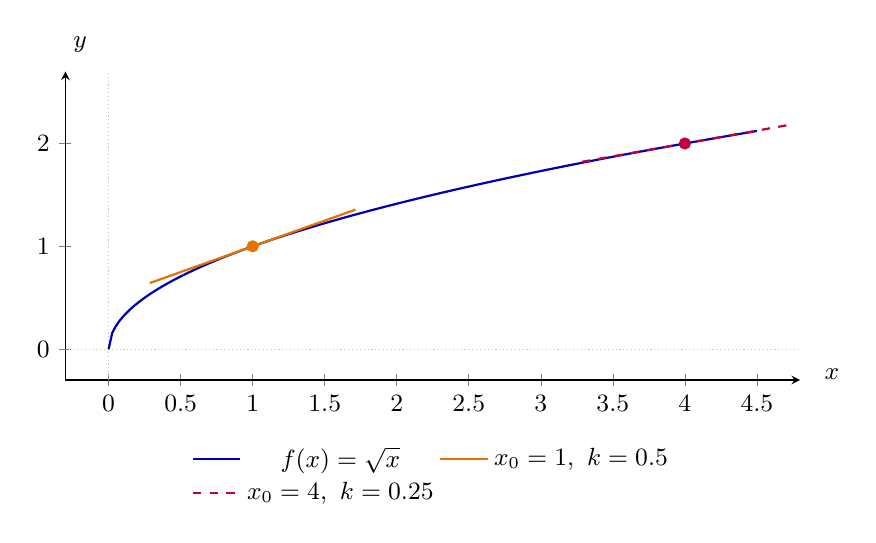
\begin{tikzpicture}[font=\small,>=stealth]
\begin{axis}[width=.90\linewidth,height=5.5cm,xmin=-0.3,xmax=4.8,ymin=-0.3,ymax=2.7,
axis lines=left,xlabel={$x$},ylabel={$y$},font=\small,
xlabel style={at={(axis description cs:1.02,.02)},anchor=west},
ylabel style={rotate=-90,at={(axis description cs:.02,1.03)},anchor=south},
legend style={at={(axis description cs:.5,-.18)},anchor=north,draw=none,fill=none,font=\small,legend columns=2},
unbounded coords=jump,clip=true,]
\addplot[gray!45,thin,densely dotted,forget plot] coordinates {(-0.3,0) (4.8,0)};
\addplot[gray!45,thin,densely dotted,forget plot] coordinates {(0,-0.3) (0,2.7)};
\addplot[blue!70!black,thick] coordinates {(0,0) (0.025,0.15811388) (0.05,0.2236068) (0.075,0.27386128) (0.1,0.31622777) (0.125,0.35355339) (0.15,0.38729833) (0.175,0.41833001) (0.2,0.4472136) (0.225,0.47434165) (0.25,0.5) (0.275,0.52440442) (0.3,0.54772256) (0.325,0.57008771) (0.35,0.59160798) (0.375,0.61237244) (0.4,0.63245553) (0.425,0.65192024) (0.45,0.67082039) (0.475,0.68920244) (0.5,0.70710678) (0.525,0.72456884) (0.55,0.74161985) (0.575,0.75828754) (0.6,0.77459667) (0.625,0.79056942) (0.65,0.80622577) (0.675,0.82158384) (0.7,0.83666003) (0.725,0.85146932) (0.75,0.8660254) (0.775,0.88034084) (0.8,0.89442719) (0.825,0.90829511) (0.85,0.92195445) (0.875,0.93541435) (0.9,0.9486833) (0.925,0.9617692) (0.95,0.97467943) (0.975,0.98742088) (1,1) (1.025,1.0124228) (1.05,1.0246951) (1.075,1.0368221) (1.1,1.0488088) (1.125,1.0606602) (1.15,1.0723805) (1.175,1.0839742) (1.2,1.0954451) (1.225,1.1067972) (1.25,1.118034) (1.275,1.129159) (1.3,1.1401754) (1.325,1.1510864) (1.35,1.161895) (1.375,1.1726039) (1.4,1.183216) (1.425,1.1937336) (1.45,1.2041595) (1.475,1.2144958) (1.5,1.2247449) (1.525,1.2349089) (1.55,1.24499) (1.575,1.25499) (1.6,1.2649111) (1.625,1.2747549) (1.65,1.2845233) (1.675,1.2942179) (1.7,1.3038405) (1.725,1.3133926) (1.75,1.3228757) (1.775,1.3322913) (1.8,1.3416408) (1.825,1.3509256) (1.85,1.3601471) (1.875,1.3693064) (1.9,1.3784049) (1.925,1.3874437) (1.95,1.396424) (1.975,1.4053469) (2,1.4142136) (2.025,1.4230249) (2.05,1.4317821) (2.075,1.440486) (2.1,1.4491377) (2.125,1.457738) (2.15,1.4662878) (2.175,1.4747881) (2.2,1.4832397) (2.225,1.4916434) (2.25,1.5) (2.275,1.5083103) (2.3,1.5165751) (2.325,1.5247951) (2.35,1.532971) (2.375,1.5411035) (2.4,1.5491933) (2.425,1.5572412) (2.45,1.5652476) (2.475,1.5732133) (2.5,1.5811388) (2.525,1.5890249) (2.55,1.5968719) (2.575,1.6046807) (2.6,1.6124515) (2.625,1.6201852) (2.65,1.6278821) (2.675,1.6355427) (2.7,1.6431677) (2.725,1.6507574) (2.75,1.6583124) (2.775,1.6658331) (2.8,1.6733201) (2.825,1.6807736) (2.85,1.6881943) (2.875,1.6955825) (2.9,1.7029386) (2.925,1.7102631) (2.95,1.7175564) (2.975,1.7248188) (3,1.7320508) (3.025,1.7392527) (3.05,1.7464249) (3.075,1.7535678) (3.1,1.7606817) (3.125,1.767767) (3.15,1.7748239) (3.175,1.781853) (3.2,1.7888544) (3.225,1.7958285) (3.25,1.8027756) (3.275,1.8096961) (3.3,1.8165902) (3.325,1.8234583) (3.35,1.8303005) (3.375,1.8371173) (3.4,1.8439089) (3.425,1.8506756) (3.45,1.8574176) (3.475,1.8641352) (3.5,1.8708287) (3.525,1.8774983) (3.55,1.8841444) (3.575,1.890767) (3.6,1.8973666) (3.625,1.9039433) (3.65,1.9104973) (3.675,1.917029) (3.7,1.9235384) (3.725,1.9300259) (3.75,1.9364917) (3.775,1.9429359) (3.8,1.9493589) (3.825,1.9557607) (3.85,1.9621417) (3.875,1.968502) (3.9,1.9748418) (3.925,1.9811613) (3.95,1.9874607) (3.975,1.9937402) (4,2) (4.025,2.0062403) (4.05,2.0124612) (4.075,2.0186629) (4.1,2.0248457) (4.125,2.0310096) (4.15,2.0371549) (4.175,2.0432817) (4.2,2.0493902) (4.225,2.0554805) (4.25,2.0615528) (4.275,2.0676073) (4.3,2.0736441) (4.325,2.0796634) (4.35,2.0856654) (4.375,2.0916501) (4.4,2.0976177) (4.425,2.1035684) (4.45,2.1095023) (4.475,2.1154196) (4.5,2.1213203)};
\addlegendentry{$f(x)=\sqrt x$}
\addplot[orange!90!black,thick] coordinates {(0.286,0.643) (1.714,1.357)};
\addlegendentry{$x_0=1,\ k=0.5$}
\addplot[only marks,mark=*,orange!90!black,forget plot] coordinates {(1,1)};
\addplot[purple,thick,dashed] coordinates {(3.286,1.8215) (4.714,2.1785)};
\addlegendentry{$x_0=4,\ k=0.25$}
\addplot[only marks,mark=*,purple,forget plot] coordinates {(4,2)};

\end{axis}
\end{tikzpicture}
\par\smallskip{\small 函数在 $x=0$ 有定义，公式的可导范围却是 $x>0$。}
\end{center}

\end{minipage}
\end{statementbox}

\begin{statementbox}
\begin{minipage}{\linewidth}
\textbf{结论6：立方根}
\[
(\sqrt[3]x)'=1/(3\sqrt[3]{x^2})
\]
% F049: native TikZ/PGFPlots, computed from the stated mathematical model.
\begin{center}
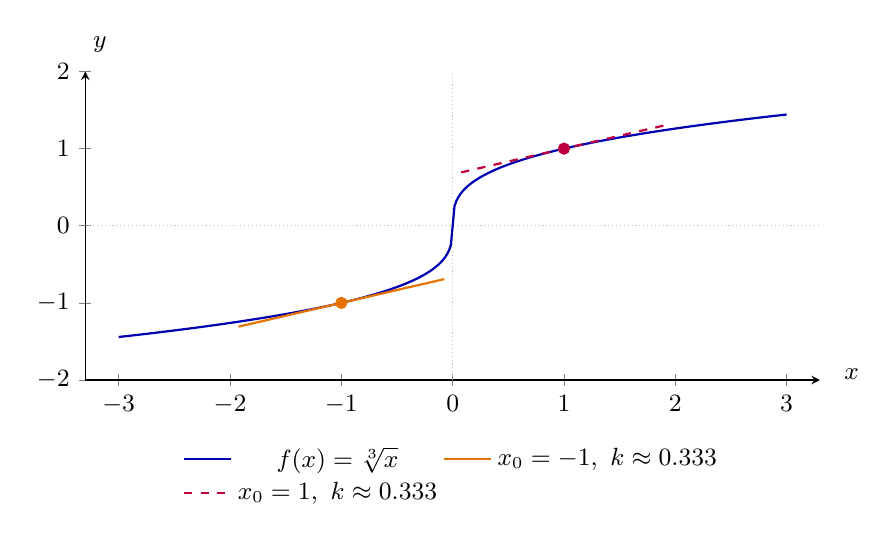
\begin{tikzpicture}[font=\small,>=stealth]
\begin{axis}[width=.90\linewidth,height=5.5cm,xmin=-3.3,xmax=3.3,ymin=-2,ymax=2,
axis lines=left,xlabel={$x$},ylabel={$y$},font=\small,
xlabel style={at={(axis description cs:1.02,.02)},anchor=west},
ylabel style={rotate=-90,at={(axis description cs:.02,1.03)},anchor=south},
legend style={at={(axis description cs:.5,-.18)},anchor=north,draw=none,fill=none,font=\small,legend columns=2},
unbounded coords=jump,clip=true,]
\addplot[gray!45,thin,densely dotted,forget plot] coordinates {(-3.3,0) (3.3,0)};
\addplot[gray!45,thin,densely dotted,forget plot] coordinates {(0,-2) (0,2)};
\addplot[blue!70!black,thick] coordinates {(-3,-1.4422496) (-2.9833333,-1.4395738) (-2.9666667,-1.436888) (-2.95,-1.4341921) (-2.9333333,-1.4314861) (-2.9166667,-1.4287698) (-2.9,-1.4260431) (-2.8833333,-1.423306) (-2.8666667,-1.4205583) (-2.85,-1.4177999) (-2.8333333,-1.4150308) (-2.8166667,-1.4122508) (-2.8,-1.4094597) (-2.7833333,-1.4066576) (-2.7666667,-1.4038443) (-2.75,-1.4010197) (-2.7333333,-1.3981836) (-2.7166667,-1.395336) (-2.7,-1.3924767) (-2.6833333,-1.3896056) (-2.6666667,-1.3867225) (-2.65,-1.3838275) (-2.6333333,-1.3809203) (-2.6166667,-1.3780008) (-2.6,-1.3750689) (-2.5833333,-1.3721244) (-2.5666667,-1.3691672) (-2.55,-1.3661972) (-2.5333333,-1.3632142) (-2.5166667,-1.3602182) (-2.5,-1.3572088) (-2.4833333,-1.3541861) (-2.4666667,-1.3511498) (-2.45,-1.3480997) (-2.4333333,-1.3450359) (-2.4166667,-1.341958) (-2.4,-1.3388659) (-2.3833333,-1.3357595) (-2.3666667,-1.3326385) (-2.35,-1.3295029) (-2.3333333,-1.3263524) (-2.3166667,-1.3231869) (-2.3,-1.3200061) (-2.2833333,-1.31681) (-2.2666667,-1.3135982) (-2.25,-1.3103707) (-2.2333333,-1.3071272) (-2.2166667,-1.3038675) (-2.2,-1.3005914) (-2.1833333,-1.2972988) (-2.1666667,-1.2939893) (-2.15,-1.2906629) (-2.1333333,-1.2873192) (-2.1166667,-1.283958) (-2.1,-1.2805792) (-2.0833333,-1.2771824) (-2.0666667,-1.2737674) (-2.05,-1.2703341) (-2.0333333,-1.2668821) (-2.0166667,-1.2634112) (-2,-1.259921) (-1.9833333,-1.2564115) (-1.9666667,-1.2528822) (-1.95,-1.249333) (-1.9333333,-1.2457634) (-1.9166667,-1.2421733) (-1.9,-1.2385623) (-1.8833333,-1.2349302) (-1.8666667,-1.2312765) (-1.85,-1.227601) (-1.8333333,-1.2239034) (-1.8166667,-1.2201833) (-1.8,-1.2164404) (-1.7833333,-1.2126743) (-1.7666667,-1.2088847) (-1.75,-1.2050711) (-1.7333333,-1.2012333) (-1.7166667,-1.1973708) (-1.7,-1.1934832) (-1.6833333,-1.1895701) (-1.6666667,-1.1856311) (-1.65,-1.1816658) (-1.6333333,-1.1776736) (-1.6166667,-1.1736542) (-1.6,-1.1696071) (-1.5833333,-1.1655318) (-1.5666667,-1.1614278) (-1.55,-1.1572945) (-1.5333333,-1.1531316) (-1.5166667,-1.1489383) (-1.5,-1.1447142) (-1.4833333,-1.1404588) (-1.4666667,-1.1361713) (-1.45,-1.1318512) (-1.4333333,-1.1274979) (-1.4166667,-1.1231107) (-1.4,-1.1186889) (-1.3833333,-1.114232) (-1.3666667,-1.109739) (-1.35,-1.1052094) (-1.3333333,-1.1006424) (-1.3166667,-1.0960372) (-1.3,-1.0913929) (-1.2833333,-1.0867087) (-1.2666667,-1.0819839) (-1.25,-1.0772173) (-1.2333333,-1.0724083) (-1.2166667,-1.0675557) (-1.2,-1.0626586) (-1.1833333,-1.0577159) (-1.1666667,-1.0527266) (-1.15,-1.0476896) (-1.1333333,-1.0426036) (-1.1166667,-1.0374675) (-1.1,-1.0322801) (-1.0833333,-1.02704) (-1.0666667,-1.0217459) (-1.05,-1.0163964) (-1.0333333,-1.0109899) (-1.0166667,-1.005525) (-1,-1) (-0.98333333,-0.99441329) (-0.96666667,-0.98876309) (-0.95,-0.98304757) (-0.93333333,-0.97726481) (-0.91666667,-0.97141278) (-0.9,-0.96548938) (-0.88333333,-0.9594924) (-0.86666667,-0.9534195) (-0.85,-0.94726824) (-0.83333333,-0.94103603) (-0.81666667,-0.93472016) (-0.8,-0.92831777) (-0.78333333,-0.92182582) (-0.76666667,-0.91524113) (-0.75,-0.9085603) (-0.73333333,-0.90177974) (-0.71666667,-0.89489566) (-0.7,-0.887904) (-0.68333333,-0.88080047) (-0.66666667,-0.87358046) (-0.65,-0.86623911) (-0.63333333,-0.85877116) (-0.61666667,-0.85117101) (-0.6,-0.84343267) (-0.58333333,-0.83554966) (-0.56666667,-0.82751503) (-0.55,-0.81932127) (-0.53333333,-0.81096027) (-0.51666667,-0.80242321) (-0.5,-0.79370053) (-0.48333333,-0.78478179) (-0.46666667,-0.77565559) (-0.45,-0.76630943) (-0.43333333,-0.75672956) (-0.41666667,-0.74690079) (-0.4,-0.7368063) (-0.38333333,-0.72642736) (-0.36666667,-0.71574306) (-0.35,-0.70472987) (-0.33333333,-0.69336127) (-0.31666667,-0.68160712) (-0.3,-0.66943295) (-0.28333333,-0.65679911) (-0.26666667,-0.64365959) (-0.25,-0.62996052) (-0.23333333,-0.61563825) (-0.21666667,-0.60061665) (-0.2,-0.58480355) (-0.18333333,-0.56808564) (-0.16666667,-0.55032121) (-0.15,-0.53132928) (-0.13333333,-0.51087295) (-0.11666667,-0.4886324) (-0.1,-0.46415888) (-0.083333333,-0.43679023) (-0.066666667,-0.40548013) (-0.05,-0.36840315) (-0.033333333,-0.32182979) (-0.016666667,-0.25543648) (0,0)};
\addlegendentry{$f(x)=\sqrt[3]x$}
\addplot[blue!70!black,thick,forget plot] coordinates {(0,0) (0.016666667,0.25543648) (0.033333333,0.32182979) (0.05,0.36840315) (0.066666667,0.40548013) (0.083333333,0.43679023) (0.1,0.46415888) (0.11666667,0.4886324) (0.13333333,0.51087295) (0.15,0.53132928) (0.16666667,0.55032121) (0.18333333,0.56808564) (0.2,0.58480355) (0.21666667,0.60061665) (0.23333333,0.61563825) (0.25,0.62996052) (0.26666667,0.64365959) (0.28333333,0.65679911) (0.3,0.66943295) (0.31666667,0.68160712) (0.33333333,0.69336127) (0.35,0.70472987) (0.36666667,0.71574306) (0.38333333,0.72642736) (0.4,0.7368063) (0.41666667,0.74690079) (0.43333333,0.75672956) (0.45,0.76630943) (0.46666667,0.77565559) (0.48333333,0.78478179) (0.5,0.79370053) (0.51666667,0.80242321) (0.53333333,0.81096027) (0.55,0.81932127) (0.56666667,0.82751503) (0.58333333,0.83554966) (0.6,0.84343267) (0.61666667,0.85117101) (0.63333333,0.85877116) (0.65,0.86623911) (0.66666667,0.87358046) (0.68333333,0.88080047) (0.7,0.887904) (0.71666667,0.89489566) (0.73333333,0.90177974) (0.75,0.9085603) (0.76666667,0.91524113) (0.78333333,0.92182582) (0.8,0.92831777) (0.81666667,0.93472016) (0.83333333,0.94103603) (0.85,0.94726824) (0.86666667,0.9534195) (0.88333333,0.9594924) (0.9,0.96548938) (0.91666667,0.97141278) (0.93333333,0.97726481) (0.95,0.98304757) (0.96666667,0.98876309) (0.98333333,0.99441329) (1,1) (1.0166667,1.005525) (1.0333333,1.0109899) (1.05,1.0163964) (1.0666667,1.0217459) (1.0833333,1.02704) (1.1,1.0322801) (1.1166667,1.0374675) (1.1333333,1.0426036) (1.15,1.0476896) (1.1666667,1.0527266) (1.1833333,1.0577159) (1.2,1.0626586) (1.2166667,1.0675557) (1.2333333,1.0724083) (1.25,1.0772173) (1.2666667,1.0819839) (1.2833333,1.0867087) (1.3,1.0913929) (1.3166667,1.0960372) (1.3333333,1.1006424) (1.35,1.1052094) (1.3666667,1.109739) (1.3833333,1.114232) (1.4,1.1186889) (1.4166667,1.1231107) (1.4333333,1.1274979) (1.45,1.1318512) (1.4666667,1.1361713) (1.4833333,1.1404588) (1.5,1.1447142) (1.5166667,1.1489383) (1.5333333,1.1531316) (1.55,1.1572945) (1.5666667,1.1614278) (1.5833333,1.1655318) (1.6,1.1696071) (1.6166667,1.1736542) (1.6333333,1.1776736) (1.65,1.1816658) (1.6666667,1.1856311) (1.6833333,1.1895701) (1.7,1.1934832) (1.7166667,1.1973708) (1.7333333,1.2012333) (1.75,1.2050711) (1.7666667,1.2088847) (1.7833333,1.2126743) (1.8,1.2164404) (1.8166667,1.2201833) (1.8333333,1.2239034) (1.85,1.227601) (1.8666667,1.2312765) (1.8833333,1.2349302) (1.9,1.2385623) (1.9166667,1.2421733) (1.9333333,1.2457634) (1.95,1.249333) (1.9666667,1.2528822) (1.9833333,1.2564115) (2,1.259921) (2.0166667,1.2634112) (2.0333333,1.2668821) (2.05,1.2703341) (2.0666667,1.2737674) (2.0833333,1.2771824) (2.1,1.2805792) (2.1166667,1.283958) (2.1333333,1.2873192) (2.15,1.2906629) (2.1666667,1.2939893) (2.1833333,1.2972988) (2.2,1.3005914) (2.2166667,1.3038675) (2.2333333,1.3071272) (2.25,1.3103707) (2.2666667,1.3135982) (2.2833333,1.31681) (2.3,1.3200061) (2.3166667,1.3231869) (2.3333333,1.3263524) (2.35,1.3295029) (2.3666667,1.3326385) (2.3833333,1.3357595) (2.4,1.3388659) (2.4166667,1.341958) (2.4333333,1.3450359) (2.45,1.3480997) (2.4666667,1.3511498) (2.4833333,1.3541861) (2.5,1.3572088) (2.5166667,1.3602182) (2.5333333,1.3632142) (2.55,1.3661972) (2.5666667,1.3691672) (2.5833333,1.3721244) (2.6,1.3750689) (2.6166667,1.3780008) (2.6333333,1.3809203) (2.65,1.3838275) (2.6666667,1.3867225) (2.6833333,1.3896056) (2.7,1.3924767) (2.7166667,1.395336) (2.7333333,1.3981836) (2.75,1.4010197) (2.7666667,1.4038443) (2.7833333,1.4066576) (2.8,1.4094597) (2.8166667,1.4122508) (2.8333333,1.4150308) (2.85,1.4177999) (2.8666667,1.4205583) (2.8833333,1.423306) (2.9,1.4260431) (2.9166667,1.4287698) (2.9333333,1.4314861) (2.95,1.4341921) (2.9666667,1.436888) (2.9833333,1.4395738) (3,1.4422496)};
\addplot[orange!90!black,thick] coordinates {(-1.924,-1.308) (-0.076,-0.692)};
\addlegendentry{$x_0=-1,\ k\approx0.333$}
\addplot[only marks,mark=*,orange!90!black,forget plot] coordinates {(-1,-1)};
\addplot[purple,thick,dashed] coordinates {(0.076,0.692) (1.924,1.308)};
\addlegendentry{$x_0=1,\ k\approx0.333$}
\addplot[only marks,mark=*,purple,forget plot] coordinates {(1,1)};

\end{axis}
\end{tikzpicture}
\par\smallskip{\small $x\ne0$；零点处差商无界，不存在有限导数。}
\end{center}

\end{minipage}
\end{statementbox}

\begin{statementbox}
\begin{minipage}{\linewidth}
\textbf{结论7：一般指数}
\[
(a^x)'=a^x\ln a
\]
% F049: native TikZ/PGFPlots, computed from the stated mathematical model.
\begin{center}
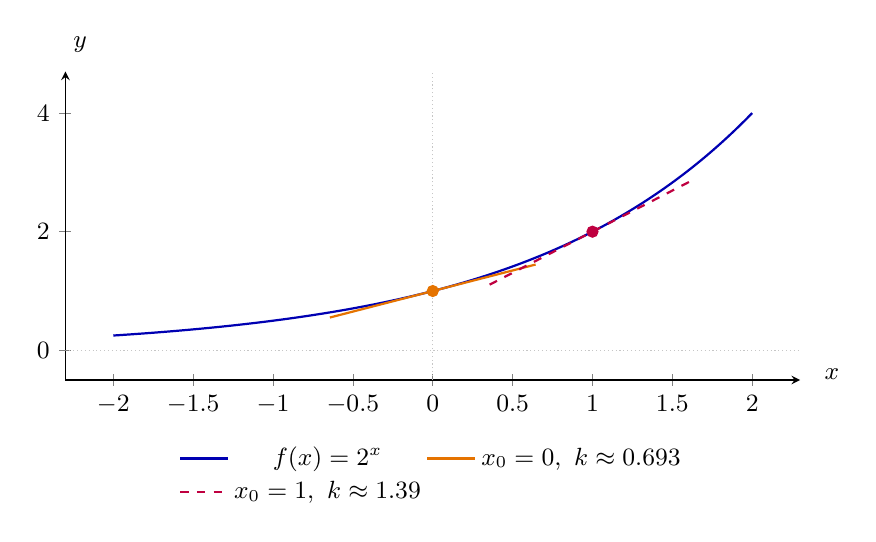
\begin{tikzpicture}[font=\small,>=stealth]
\begin{axis}[width=.90\linewidth,height=5.5cm,xmin=-2.3,xmax=2.3,ymin=-0.5,ymax=4.7,
axis lines=left,xlabel={$x$},ylabel={$y$},font=\small,
xlabel style={at={(axis description cs:1.02,.02)},anchor=west},
ylabel style={rotate=-90,at={(axis description cs:.02,1.03)},anchor=south},
legend style={at={(axis description cs:.5,-.18)},anchor=north,draw=none,fill=none,font=\small,legend columns=2},
unbounded coords=jump,clip=true,]
\addplot[gray!45,thin,densely dotted,forget plot] coordinates {(-2.3,0) (2.3,0)};
\addplot[gray!45,thin,densely dotted,forget plot] coordinates {(0,-0.5) (0,4.7)};
\addplot[blue!70!black,thick] coordinates {(-2,0.25) (-1.9777778,0.25388063) (-1.9555556,0.25782149) (-1.9333333,0.26182353) (-1.9111111,0.26588769) (-1.8888889,0.27001493) (-1.8666667,0.27420624) (-1.8444444,0.27846261) (-1.8222222,0.28278505) (-1.8,0.28717459) (-1.7777778,0.29163226) (-1.7555556,0.29615913) (-1.7333333,0.30075626) (-1.7111111,0.30542475) (-1.6888889,0.31016571) (-1.6666667,0.31498026) (-1.6444444,0.31986955) (-1.6222222,0.32483473) (-1.6,0.32987698) (-1.5777778,0.3349975) (-1.5555556,0.3401975) (-1.5333333,0.34547822) (-1.5111111,0.35084091) (-1.4888889,0.35628684) (-1.4666667,0.36181731) (-1.4444444,0.36743362) (-1.4222222,0.37313712) (-1.4,0.37892914) (-1.3777778,0.38481107) (-1.3555556,0.39078431) (-1.3333333,0.39685026) (-1.3111111,0.40301038) (-1.2888889,0.40926611) (-1.2666667,0.41561895) (-1.2444444,0.4220704) (-1.2222222,0.42862199) (-1.2,0.43527528) (-1.1777778,0.44203185) (-1.1555556,0.44889329) (-1.1333333,0.45586124) (-1.1111111,0.46293736) (-1.0888889,0.47012331) (-1.0666667,0.4774208) (-1.0444444,0.48483157) (-1.0222222,0.49235738) (-1,0.5) (-0.97777778,0.50776126) (-0.95555556,0.51564299) (-0.93333333,0.52364706) (-0.91111111,0.53177538) (-0.88888889,0.54002987) (-0.86666667,0.54841249) (-0.84444444,0.55692523) (-0.82222222,0.56557011) (-0.8,0.57434918) (-0.77777778,0.58326452) (-0.75555556,0.59231825) (-0.73333333,0.60151252) (-0.71111111,0.6108495) (-0.68888889,0.62033142) (-0.66666667,0.62996052) (-0.64444444,0.6397391) (-0.62222222,0.64966945) (-0.6,0.65975396) (-0.57777778,0.66999499) (-0.55555556,0.680395) (-0.53333333,0.69095644) (-0.51111111,0.70168182) (-0.48888889,0.71257368) (-0.46666667,0.72363462) (-0.44444444,0.73486725) (-0.42222222,0.74627423) (-0.4,0.75785828) (-0.37777778,0.76962215) (-0.35555556,0.78156862) (-0.33333333,0.79370053) (-0.31111111,0.80602075) (-0.28888889,0.81853222) (-0.26666667,0.8312379) (-0.24444444,0.8441408) (-0.22222222,0.85724398) (-0.2,0.87055056) (-0.17777778,0.8840637) (-0.15555556,0.89778659) (-0.13333333,0.91172249) (-0.11111111,0.92587471) (-0.088888889,0.94024661) (-0.066666667,0.9548416) (-0.044444444,0.96966314) (-0.022222222,0.98471475) (0,1) (0.022222222,1.0155225) (0.044444444,1.031286) (0.066666667,1.0472941) (0.088888889,1.0635508) (0.11111111,1.0800597) (0.13333333,1.096825) (0.15555556,1.1138505) (0.17777778,1.1311402) (0.2,1.1486984) (0.22222222,1.166529) (0.24444444,1.1846365) (0.26666667,1.203025) (0.28888889,1.221699) (0.31111111,1.2406628) (0.33333333,1.259921) (0.35555556,1.2794782) (0.37777778,1.2993389) (0.4,1.3195079) (0.42222222,1.33999) (0.44444444,1.36079) (0.46666667,1.3819129) (0.48888889,1.4033636) (0.51111111,1.4251474) (0.53333333,1.4472692) (0.55555556,1.4697345) (0.57777778,1.4925485) (0.6,1.5157166) (0.62222222,1.5392443) (0.64444444,1.5631372) (0.66666667,1.5874011) (0.68888889,1.6120415) (0.71111111,1.6370644) (0.73333333,1.6624758) (0.75555556,1.6882816) (0.77777778,1.714488) (0.8,1.7411011) (0.82222222,1.7681274) (0.84444444,1.7955732) (0.86666667,1.823445) (0.88888889,1.8517494) (0.91111111,1.8804932) (0.93333333,1.9096832) (0.95555556,1.9393263) (0.97777778,1.9694295) (1,2) (1.0222222,2.031045) (1.0444444,2.0625719) (1.0666667,2.0945882) (1.0888889,2.1271015) (1.1111111,2.1601195) (1.1333333,2.19365) (1.1555556,2.2277009) (1.1777778,2.2622804) (1.2,2.2973967) (1.2222222,2.3330581) (1.2444444,2.369273) (1.2666667,2.4060501) (1.2888889,2.443398) (1.3111111,2.4813257) (1.3333333,2.5198421) (1.3555556,2.5589564) (1.3777778,2.5986778) (1.4,2.6390158) (1.4222222,2.67998) (1.4444444,2.72158) (1.4666667,2.7638258) (1.4888889,2.8067273) (1.5111111,2.8502947) (1.5333333,2.8945385) (1.5555556,2.939469) (1.5777778,2.9850969) (1.6,3.0314331) (1.6222222,3.0784886) (1.6444444,3.1262745) (1.6666667,3.1748021) (1.6888889,3.224083) (1.7111111,3.2741289) (1.7333333,3.3249516) (1.7555556,3.3765632) (1.7777778,3.4289759) (1.8,3.4822023) (1.8222222,3.5362548) (1.8444444,3.5911463) (1.8666667,3.64689) (1.8888889,3.7034988) (1.9111111,3.7609865) (1.9333333,3.8193664) (1.9555556,3.8786526) (1.9777778,3.938859) (2,4)};
\addlegendentry{$f(x)=2^x$}
\addplot[orange!90!black,thick] coordinates {(-0.644,0.55361322) (0.644,1.4463868)};
\addlegendentry{$x_0=0,\ k\approx0.693$}
\addplot[only marks,mark=*,orange!90!black,forget plot] coordinates {(0,1)};
\addplot[purple,thick,dashed] coordinates {(0.356,1.1072264) (1.644,2.8927736)};
\addlegendentry{$x_0=1,\ k\approx1.39$}
\addplot[only marks,mark=*,purple,forget plot] coordinates {(1,2)};

\end{axis}
\end{tikzpicture}
\par\smallskip{\small $a>0$；图中取 $a=2$，一般底数的正负变化见易错一。}
\end{center}

\end{minipage}
$a=1$ 时 $1^x$ 为常数，导数为零，公式仍成立；但 $\log_1x$ 不存在。
\end{statementbox}

\begin{statementbox}
\begin{minipage}{\linewidth}
\textbf{结论8：自然指数}
\[
(e^x)'=e^x
\]
% F049: native TikZ/PGFPlots, computed from the stated mathematical model.
\begin{center}
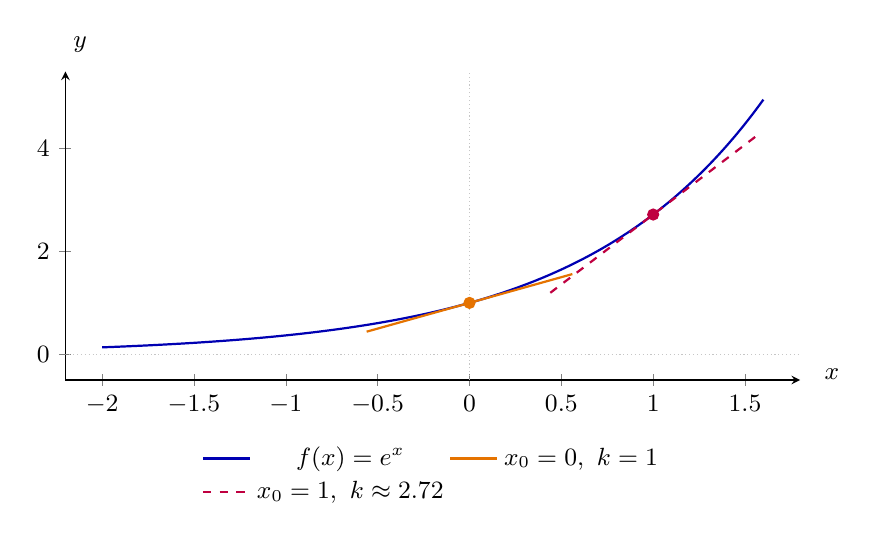
\begin{tikzpicture}[font=\small,>=stealth]
\begin{axis}[width=.90\linewidth,height=5.5cm,xmin=-2.2,xmax=1.8,ymin=-0.5,ymax=5.5,
axis lines=left,xlabel={$x$},ylabel={$y$},font=\small,
xlabel style={at={(axis description cs:1.02,.02)},anchor=west},
ylabel style={rotate=-90,at={(axis description cs:.02,1.03)},anchor=south},
legend style={at={(axis description cs:.5,-.18)},anchor=north,draw=none,fill=none,font=\small,legend columns=2},
unbounded coords=jump,clip=true,]
\addplot[gray!45,thin,densely dotted,forget plot] coordinates {(-2.2,0) (1.8,0)};
\addplot[gray!45,thin,densely dotted,forget plot] coordinates {(0,-0.5) (0,5.5)};
\addplot[blue!70!black,thick] coordinates {(-2,0.13533528) (-1.98,0.13806924) (-1.96,0.14085842) (-1.94,0.14370395) (-1.92,0.14660696) (-1.9,0.14956862) (-1.88,0.15259011) (-1.86,0.15567263) (-1.84,0.15881743) (-1.82,0.16202575) (-1.8,0.16529889) (-1.78,0.16863815) (-1.76,0.17204486) (-1.74,0.1755204) (-1.72,0.17906615) (-1.7,0.18268352) (-1.68,0.18637398) (-1.66,0.19013898) (-1.64,0.19398004) (-1.62,0.1978987) (-1.6,0.20189652) (-1.58,0.2059751) (-1.56,0.21013607) (-1.54,0.2143811) (-1.52,0.21871189) (-1.5,0.22313016) (-1.48,0.22763769) (-1.46,0.23223627) (-1.44,0.23692776) (-1.42,0.24171402) (-1.4,0.24659696) (-1.38,0.25157855) (-1.36,0.25666078) (-1.34,0.26184567) (-1.32,0.2671353) (-1.3,0.27253179) (-1.28,0.2780373) (-1.26,0.28365403) (-1.24,0.28938422) (-1.22,0.29523017) (-1.2,0.30119421) (-1.18,0.30727874) (-1.16,0.31348618) (-1.14,0.31981902) (-1.12,0.32627979) (-1.1,0.33287108) (-1.08,0.33959553) (-1.06,0.34645581) (-1.04,0.35345468) (-1.02,0.36059494) (-1,0.36787944) (-0.98,0.3753111) (-0.96,0.38289289) (-0.94,0.39062784) (-0.92,0.39851904) (-0.9,0.40656966) (-0.88,0.41478291) (-0.86,0.42316208) (-0.84,0.43171052) (-0.82,0.44043165) (-0.8,0.44932896) (-0.78,0.45840601) (-0.76,0.46766643) (-0.74,0.47711392) (-0.72,0.48675226) (-0.7,0.4965853) (-0.68,0.50661699) (-0.66,0.51685133) (-0.64,0.52729242) (-0.62,0.53794444) (-0.6,0.54881164) (-0.58,0.55989837) (-0.56,0.57120906) (-0.54,0.58274825) (-0.52,0.59452055) (-0.5,0.60653066) (-0.48,0.61878339) (-0.46,0.63128365) (-0.44,0.64403642) (-0.42,0.65704682) (-0.4,0.67032005) (-0.38,0.68386141) (-0.36,0.69767633) (-0.34,0.71177032) (-0.32,0.72614904) (-0.3,0.74081822) (-0.28,0.75578374) (-0.26,0.77105159) (-0.24,0.78662786) (-0.22,0.8025188) (-0.2,0.81873075) (-0.18,0.83527021) (-0.16,0.85214379) (-0.14,0.86935824) (-0.12,0.88692044) (-0.1,0.90483742) (-0.08,0.92311635) (-0.06,0.94176453) (-0.04,0.96078944) (-0.02,0.98019867) (0,1) (0.02,1.0202013) (0.04,1.0408108) (0.06,1.0618365) (0.08,1.0832871) (0.1,1.1051709) (0.12,1.1274969) (0.14,1.1502738) (0.16,1.1735109) (0.18,1.1972174) (0.2,1.2214028) (0.22,1.2460767) (0.24,1.2712492) (0.26,1.2969301) (0.28,1.3231298) (0.3,1.3498588) (0.32,1.3771278) (0.34,1.4049476) (0.36,1.4333294) (0.38,1.4622846) (0.4,1.4918247) (0.42,1.5219616) (0.44,1.5527072) (0.46,1.584074) (0.48,1.6160744) (0.5,1.6487213) (0.52,1.6820276) (0.54,1.7160069) (0.56,1.7506725) (0.58,1.7860384) (0.6,1.8221188) (0.62,1.858928) (0.64,1.8964809) (0.66,1.9347923) (0.68,1.9738777) (0.7,2.0137527) (0.72,2.0544332) (0.74,2.0959355) (0.76,2.1382762) (0.78,2.1814723) (0.8,2.2255409) (0.82,2.2704998) (0.84,2.316367) (0.86,2.3631607) (0.88,2.4108997) (0.9,2.4596031) (0.92,2.5092904) (0.94,2.5599814) (0.96,2.6116965) (0.98,2.6644562) (1,2.7182818) (1.02,2.7731948) (1.04,2.829217) (1.06,2.886371) (1.08,2.9446796) (1.1,3.004166) (1.12,3.0648542) (1.14,3.1267684) (1.16,3.1899333) (1.18,3.2543742) (1.2,3.3201169) (1.22,3.3871877) (1.24,3.4556135) (1.26,3.5254215) (1.28,3.5966397) (1.3,3.6692967) (1.32,3.7434214) (1.34,3.8190435) (1.36,3.8961933) (1.38,3.9749016) (1.4,4.0552) (1.42,4.1371204) (1.44,4.2206958) (1.46,4.3059595) (1.48,4.3929457) (1.5,4.4816891) (1.52,4.5722252) (1.54,4.6645903) (1.56,4.7588212) (1.58,4.8549558) (1.6,4.9530324)};
\addlegendentry{$f(x)=e^x$}
\addplot[orange!90!black,thick] coordinates {(-0.56,0.44) (0.56,1.56)};
\addlegendentry{$x_0=0,\ k=1$}
\addplot[only marks,mark=*,orange!90!black,forget plot] coordinates {(0,1)};
\addplot[purple,thick,dashed] coordinates {(0.44,1.196044) (1.56,4.2405197)};
\addlegendentry{$x_0=1,\ k\approx2.72$}
\addplot[only marks,mark=*,purple,forget plot] coordinates {(1,2.7182818)};

\end{axis}
\end{tikzpicture}
\par\smallskip{\small 任意实数 $x$；每一点的切线斜率等于该点的函数值。}
\end{center}

\end{minipage}
\end{statementbox}

\begin{statementbox}
\begin{minipage}{\linewidth}
\textbf{结论9：一般对数}
\[
(\log_a x)'=1/(x\ln a)
\]
% F049: native TikZ/PGFPlots, computed from the stated mathematical model.
\begin{center}
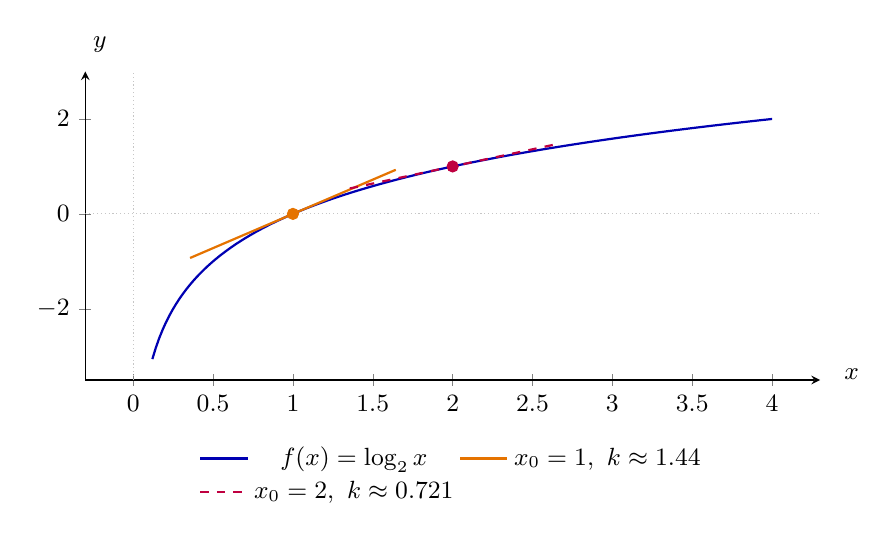
\begin{tikzpicture}[font=\small,>=stealth]
\begin{axis}[width=.90\linewidth,height=5.5cm,xmin=-0.3,xmax=4.3,ymin=-3.5,ymax=3,
axis lines=left,xlabel={$x$},ylabel={$y$},font=\small,
xlabel style={at={(axis description cs:1.02,.02)},anchor=west},
ylabel style={rotate=-90,at={(axis description cs:.02,1.03)},anchor=south},
legend style={at={(axis description cs:.5,-.18)},anchor=north,draw=none,fill=none,font=\small,legend columns=2},
unbounded coords=jump,clip=true,]
\addplot[gray!45,thin,densely dotted,forget plot] coordinates {(-0.3,0) (4.3,0)};
\addplot[gray!45,thin,densely dotted,forget plot] coordinates {(0,-3.5) (0,3)};
\addplot[blue!70!black,thick] coordinates {(0.12,-3.0588937) (0.14155556,-2.8205597) (0.16311111,-2.616073) (0.18466667,-2.4370046) (0.20622222,-2.2777283) (0.22777778,-2.1343011) (0.24933333,-2.0038523) (0.27088889,-1.8842269) (0.29244444,-1.7737655) (0.314,-1.6711635) (0.33555556,-1.5753765) (0.35711111,-1.4855551) (0.37866667,-1.4009997) (0.40022222,-1.3211268) (0.42177778,-1.245445) (0.44333333,-1.1735363) (0.46488889,-1.1050421) (0.48644444,-1.039653) (0.508,-0.9770996) (0.52955556,-0.91714605) (0.55111111,-0.85958488) (0.57266667,-0.80423246) (0.59422222,-0.75092554) (0.61577778,-0.69951829) (0.63733333,-0.64987998) (0.65888889,-0.6018929) (0.68044444,-0.55545072) (0.702,-0.51045706) (0.72355556,-0.4668243) (0.74511111,-0.42447252) (0.76666667,-0.38332864) (0.78822222,-0.34332567) (0.80977778,-0.30440204) (0.83133333,-0.26650104) (0.85288889,-0.22957029) (0.87444444,-0.19356137) (0.896,-0.15842936) (0.91755556,-0.12413258) (0.93911111,-0.090632234) (0.96066667,-0.057892165) (0.98222222,-0.025878632) (1.0037778,0.0054399123) (1.0253333,0.036093003) (1.0468889,0.066108331) (1.0684444,0.095511895) (1.09,0.12432814) (1.1115556,0.15258006) (1.1331111,0.18028934) (1.1546667,0.20747643) (1.1762222,0.23416065) (1.1977778,0.26036027) (1.2193333,0.28609257) (1.2408889,0.31137394) (1.2624444,0.3362199) (1.284,0.3606452) (1.3055556,0.38466385) (1.3271111,0.40828916) (1.3486667,0.43153382) (1.3702222,0.45440989) (1.3917778,0.47692888) (1.4133333,0.49910176) (1.4348889,0.52093903) (1.4564444,0.54245067) (1.478,0.56364627) (1.4995556,0.58453497) (1.5211111,0.60512554) (1.5426667,0.62542636) (1.5642222,0.64544548) (1.5857778,0.66519061) (1.6073333,0.68466915) (1.6288889,0.7038882) (1.6504444,0.72285458) (1.672,0.74157485) (1.6935556,0.76005531) (1.7151111,0.77830204) (1.7366667,0.79632087) (1.7582222,0.81411742) (1.7797778,0.83169712) (1.8013333,0.84906517) (1.8228889,0.86622663) (1.8444444,0.88318634) (1.866,0.89994899) (1.8875556,0.91651911) (1.9091111,0.93290107) (1.9306667,0.9490991) (1.9522222,0.96511728) (1.9737778,0.98095957) (1.9953333,0.99662978) (2.0168889,1.0121316) (2.0384444,1.0274686) (2.06,1.0426443) (2.0815556,1.0576621) (2.1031111,1.0725251) (2.1246667,1.0872365) (2.1462222,1.1017995) (2.1677778,1.1162169) (2.1893333,1.1304916) (2.2108889,1.1446265) (2.2324444,1.1586243) (2.254,1.1724875) (2.2755556,1.1862188) (2.2971111,1.1998206) (2.3186667,1.2132954) (2.3402222,1.2266455) (2.3617778,1.2398732) (2.3833333,1.2529807) (2.4048889,1.2659702) (2.4264444,1.2788438) (2.448,1.2916036) (2.4695556,1.3042514) (2.4911111,1.3167894) (2.5126667,1.3292193) (2.5342222,1.341543) (2.5557778,1.3537624) (2.5773333,1.3658791) (2.5988889,1.377895) (2.6204444,1.3898115) (2.642,1.4016305) (2.6635556,1.4133534) (2.6851111,1.4249818) (2.7066667,1.4365172) (2.7282222,1.4479612) (2.7497778,1.459315) (2.7713333,1.4705802) (2.7928889,1.4817582) (2.8144444,1.4928502) (2.836,1.5038575) (2.8575556,1.5147815) (2.8791111,1.5256235) (2.9006667,1.5363845) (2.9222222,1.5470659) (2.9437778,1.5576688) (2.9653333,1.5681943) (2.9868889,1.5786436) (3.0084444,1.5890177) (3.03,1.5993178) (3.0515556,1.6095449) (3.0731111,1.6196999) (3.0946667,1.629784) (3.1162222,1.6397981) (3.1377778,1.6497432) (3.1593333,1.6596202) (3.1808889,1.66943) (3.2024444,1.6791735) (3.224,1.6888517) (3.2455556,1.6984655) (3.2671111,1.7080155) (3.2886667,1.7175028) (3.3102222,1.7269281) (3.3317778,1.7362922) (3.3533333,1.7455959) (3.3748889,1.75484) (3.3964444,1.7640253) (3.418,1.7731524) (3.4395556,1.7822222) (3.4611111,1.7912353) (3.4826667,1.8001924) (3.5042222,1.8090943) (3.5257778,1.8179415) (3.5473333,1.8267349) (3.5688889,1.835475) (3.5904444,1.8441624) (3.612,1.8527979) (3.6335556,1.861382) (3.6551111,1.8699153) (3.6766667,1.8783984) (3.6982222,1.8868319) (3.7197778,1.8952164) (3.7413333,1.9035525) (3.7628889,1.9118407) (3.7844444,1.9200815) (3.806,1.9282756) (3.8275556,1.9364233) (3.8491111,1.9445253) (3.8706667,1.9525821) (3.8922222,1.9605941) (3.9137778,1.9685618) (3.9353333,1.9764858) (3.9568889,1.9843666) (3.9784444,1.9922045) (4,2)};
\addlegendentry{$f(x)=\log_2x$}
\addplot[orange!90!black,thick] coordinates {(0.356,-0.92909561) (1.644,0.92909561)};
\addlegendentry{$x_0=1,\ k\approx1.44$}
\addplot[only marks,mark=*,orange!90!black,forget plot] coordinates {(1,0)};
\addplot[purple,thick,dashed] coordinates {(1.356,0.5354522) (2.644,1.4645478)};
\addlegendentry{$x_0=2,\ k\approx0.721$}
\addplot[only marks,mark=*,purple,forget plot] coordinates {(2,1)};

\end{axis}
\end{tikzpicture}
\par\smallskip{\small $x>0$，$a>0,a\ne1$；图中取 $a=2$，换底带来因子 $1/\ln2$。}
\end{center}

\end{minipage}
\end{statementbox}

\begin{statementbox}
\begin{minipage}{\linewidth}
\textbf{结论10：自然对数}
\[
(\ln x)'=1/x
\]
% F049: native TikZ/PGFPlots, computed from the stated mathematical model.
\begin{center}
\begin{tikzpicture}[font=\small,>=stealth]
\begin{axis}[width=.90\linewidth,height=5.5cm,xmin=-0.3,xmax=4.3,ymin=-2.5,ymax=2,
axis lines=left,xlabel={$x$},ylabel={$y$},font=\small,
xlabel style={at={(axis description cs:1.02,.02)},anchor=west},
ylabel style={rotate=-90,at={(axis description cs:.02,1.03)},anchor=south},
legend style={at={(axis description cs:.5,-.18)},anchor=north,draw=none,fill=none,font=\small,legend columns=2},
unbounded coords=jump,clip=true,]
\addplot[gray!45,thin,densely dotted,forget plot] coordinates {(-0.3,0) (4.3,0)};
\addplot[gray!45,thin,densely dotted,forget plot] coordinates {(0,-2.5) (0,2)};
\addplot[blue!70!black,thick] coordinates {(0.12,-2.1202635) (0.14155556,-1.955063) (0.16311111,-1.8133236) (0.18466667,-1.6892029) (0.20622222,-1.5788009) (0.22777778,-1.4793848) (0.24933333,-1.3889646) (0.27088889,-1.3060465) (0.29244444,-1.2294806) (0.314,-1.1583623) (0.33555556,-1.0919677) (0.35711111,-1.0297083) (0.37866667,-0.97109897) (0.40022222,-0.91573533) (0.42177778,-0.8632767) (0.44333333,-0.81343335) (0.46488889,-0.76595685) (0.48644444,-0.72063258) (0.508,-0.67727383) (0.52955556,-0.6357172) (0.55111111,-0.59581884) (0.57266667,-0.55745147) (0.59422222,-0.52050192) (0.61577778,-0.48486913) (0.63733333,-0.45046247) (0.65888889,-0.41720036) (0.68044444,-0.3850091) (0.702,-0.35382187) (0.72355556,-0.32357795) (0.74511111,-0.29422193) (0.76666667,-0.26570317) (0.78822222,-0.23797522) (0.80977778,-0.21099542) (0.83133333,-0.18472444) (0.85288889,-0.159126) (0.87444444,-0.13416651) (0.896,-0.10981487) (0.91755556,-0.08604215) (0.93911111,-0.062821478) (0.96066667,-0.040127791) (0.98222222,-0.017937701) (1.0037778,0.0037706599) (1.0253333,0.025017763) (1.0468889,0.045822803) (1.0684444,0.0662038) (1.09,0.086177696) (1.1115556,0.10576044) (1.1331111,0.12496705) (1.1546667,0.1438117) (1.1762222,0.1623078) (1.1977778,0.18046799) (1.2193333,0.19830426) (1.2408889,0.21582797) (1.2624444,0.23304988) (1.284,0.24998021) (1.3055556,0.26662866) (1.3271111,0.28300448) (1.3486667,0.29911645) (1.3702222,0.31497293) (1.3917778,0.33058191) (1.4133333,0.34595098) (1.4348889,0.36108742) (1.4564444,0.37599815) (1.478,0.39068982) (1.4995556,0.40516877) (1.5211111,0.41944106) (1.5426667,0.43351252) (1.5642222,0.44738872) (1.5857778,0.461075) (1.6073333,0.47457649) (1.6288889,0.48789812) (1.6504444,0.50104461) (1.672,0.51402051) (1.6935556,0.5268302) (1.7151111,0.53947787) (1.7366667,0.55196757) (1.7582222,0.5643032) (1.7797778,0.57648851) (1.8013333,0.58852713) (1.8228889,0.60042254) (1.8444444,0.61217812) (1.866,0.6237971) (1.8875556,0.63528264) (1.9091111,0.64663775) (1.9306667,0.65786537) (1.9522222,0.66896832) (1.9737778,0.67994936) (1.9953333,0.69081112) (2.0168889,0.70155617) (2.0384444,0.71218699) (2.06,0.72270598) (2.0815556,0.73311548) (2.1031111,0.74341773) (2.1246667,0.75361493) (2.1462222,0.76370919) (2.1677778,0.77370258) (2.1893333,0.78359708) (2.2108889,0.79339465) (2.2324444,0.80309715) (2.254,0.81270642) (2.2755556,0.82222422) (2.2971111,0.83165229) (2.3186667,0.84099231) (2.3402222,0.85024589) (2.3617778,0.85941463) (2.3833333,0.86850007) (2.4048889,0.8775037) (2.4264444,0.88642699) (2.448,0.89527136) (2.4695556,0.9040382) (2.4911111,0.91272884) (2.5126667,0.92134461) (2.5342222,0.92988677) (2.5557778,0.93835659) (2.5773333,0.94675527) (2.5988889,0.955084) (2.6204444,0.96334394) (2.642,0.97153621) (2.6635556,0.97966191) (2.6851111,0.98772211) (2.7066667,0.99571787) (2.7282222,1.0036502) (2.7497778,1.0115201) (2.7713333,1.0193286) (2.7928889,1.0270765) (2.8144444,1.0347649) (2.836,1.0423946) (2.8575556,1.0499666) (2.8791111,1.0574816) (2.9006667,1.0649406) (2.9222222,1.0723444) (2.9437778,1.0796937) (2.9653333,1.0869894) (2.9868889,1.0942323) (3.0084444,1.1014231) (3.03,1.1085626) (3.0515556,1.1156515) (3.0731111,1.1226904) (3.0946667,1.1296802) (3.1162222,1.1366214) (3.1377778,1.1435148) (3.1593333,1.150361) (3.1808889,1.1571607) (3.2024444,1.1639144) (3.224,1.1706228) (3.2455556,1.1772865) (3.2671111,1.1839061) (3.2886667,1.1904822) (3.3102222,1.1970153) (3.3317778,1.203506) (3.3533333,1.2099549) (3.3748889,1.2163624) (3.3964444,1.2227291) (3.418,1.2290556) (3.4395556,1.2353423) (3.4611111,1.2415897) (3.4826667,1.2477983) (3.5042222,1.2539686) (3.5257778,1.2601011) (3.5473333,1.2661961) (3.5688889,1.2722543) (3.5904444,1.278276) (3.612,1.2842616) (3.6335556,1.2902117) (3.6551111,1.2961265) (3.6766667,1.3020065) (3.6982222,1.3078522) (3.7197778,1.3136639) (3.7413333,1.3194421) (3.7628889,1.325187) (3.7844444,1.3308991) (3.806,1.3365788) (3.8275556,1.3422264) (3.8491111,1.3478422) (3.8706667,1.3534268) (3.8922222,1.3589803) (3.9137778,1.3645031) (3.9353333,1.3699956) (3.9568889,1.3754581) (3.9784444,1.3808909) (4,1.3862944)};
\addlegendentry{$f(x)=\ln x$}
\addplot[orange!90!black,thick] coordinates {(0.356,-0.644) (1.644,0.644)};
\addlegendentry{$x_0=1,\ k=1$}
\addplot[only marks,mark=*,orange!90!black,forget plot] coordinates {(1,0)};
\addplot[purple,thick,dashed] coordinates {(1.356,0.37114718) (2.644,1.0151472)};
\addlegendentry{$x_0=2,\ k=0.5$}
\addplot[only marks,mark=*,purple,forget plot] coordinates {(2,0.69314718)};

\end{axis}
\end{tikzpicture}
\par\smallskip{\small $x>0$；越向右，切线越平缓。}
\end{center}

\end{minipage}
\end{statementbox}

\begin{statementbox}
\begin{minipage}{\linewidth}
\textbf{结论11：绝对值对数}
\[
(\ln|x|)'=1/x
\]
% F049: native TikZ/PGFPlots, computed from the stated mathematical model.
\begin{center}
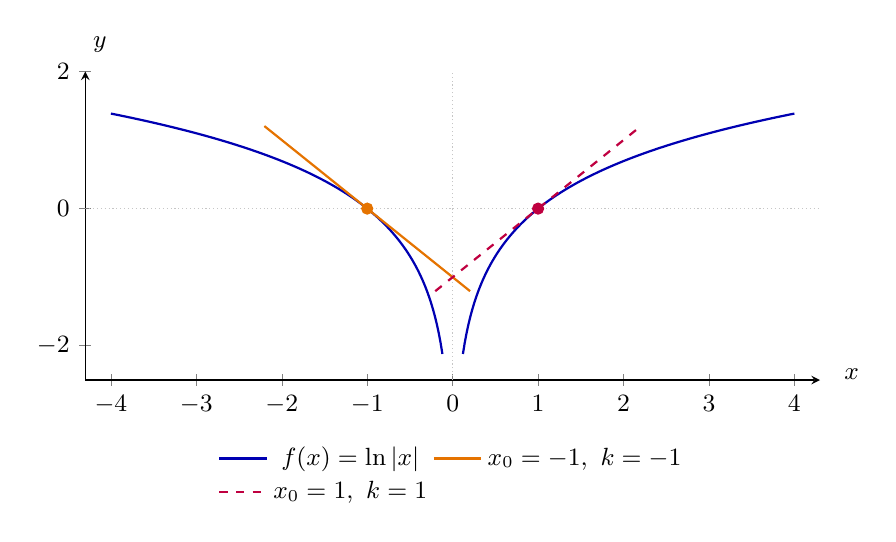
\begin{tikzpicture}[font=\small,>=stealth]
\begin{axis}[width=.90\linewidth,height=5.5cm,xmin=-4.3,xmax=4.3,ymin=-2.5,ymax=2,
axis lines=left,xlabel={$x$},ylabel={$y$},font=\small,
xlabel style={at={(axis description cs:1.02,.02)},anchor=west},
ylabel style={rotate=-90,at={(axis description cs:.02,1.03)},anchor=south},
legend style={at={(axis description cs:.5,-.18)},anchor=north,draw=none,fill=none,font=\small,legend columns=2},
unbounded coords=jump,clip=true,]
\addplot[gray!45,thin,densely dotted,forget plot] coordinates {(-4.3,0) (4.3,0)};
\addplot[gray!45,thin,densely dotted,forget plot] coordinates {(0,-2.5) (0,2)};
\addplot[blue!70!black,thick] coordinates {(-4,1.3862944) (-3.9784444,1.3808909) (-3.9568889,1.3754581) (-3.9353333,1.3699956) (-3.9137778,1.3645031) (-3.8922222,1.3589803) (-3.8706667,1.3534268) (-3.8491111,1.3478422) (-3.8275556,1.3422264) (-3.806,1.3365788) (-3.7844444,1.3308991) (-3.7628889,1.325187) (-3.7413333,1.3194421) (-3.7197778,1.3136639) (-3.6982222,1.3078522) (-3.6766667,1.3020065) (-3.6551111,1.2961265) (-3.6335556,1.2902117) (-3.612,1.2842616) (-3.5904444,1.278276) (-3.5688889,1.2722543) (-3.5473333,1.2661961) (-3.5257778,1.2601011) (-3.5042222,1.2539686) (-3.4826667,1.2477983) (-3.4611111,1.2415897) (-3.4395556,1.2353423) (-3.418,1.2290556) (-3.3964444,1.2227291) (-3.3748889,1.2163624) (-3.3533333,1.2099549) (-3.3317778,1.203506) (-3.3102222,1.1970153) (-3.2886667,1.1904822) (-3.2671111,1.1839061) (-3.2455556,1.1772865) (-3.224,1.1706228) (-3.2024444,1.1639144) (-3.1808889,1.1571607) (-3.1593333,1.150361) (-3.1377778,1.1435148) (-3.1162222,1.1366214) (-3.0946667,1.1296802) (-3.0731111,1.1226904) (-3.0515556,1.1156515) (-3.03,1.1085626) (-3.0084444,1.1014231) (-2.9868889,1.0942323) (-2.9653333,1.0869894) (-2.9437778,1.0796937) (-2.9222222,1.0723444) (-2.9006667,1.0649406) (-2.8791111,1.0574816) (-2.8575556,1.0499666) (-2.836,1.0423946) (-2.8144444,1.0347649) (-2.7928889,1.0270765) (-2.7713333,1.0193286) (-2.7497778,1.0115201) (-2.7282222,1.0036502) (-2.7066667,0.99571787) (-2.6851111,0.98772211) (-2.6635556,0.97966191) (-2.642,0.97153621) (-2.6204444,0.96334394) (-2.5988889,0.955084) (-2.5773333,0.94675527) (-2.5557778,0.93835659) (-2.5342222,0.92988677) (-2.5126667,0.92134461) (-2.4911111,0.91272884) (-2.4695556,0.9040382) (-2.448,0.89527136) (-2.4264444,0.88642699) (-2.4048889,0.8775037) (-2.3833333,0.86850007) (-2.3617778,0.85941463) (-2.3402222,0.85024589) (-2.3186667,0.84099231) (-2.2971111,0.83165229) (-2.2755556,0.82222422) (-2.254,0.81270642) (-2.2324444,0.80309715) (-2.2108889,0.79339465) (-2.1893333,0.78359708) (-2.1677778,0.77370258) (-2.1462222,0.76370919) (-2.1246667,0.75361493) (-2.1031111,0.74341773) (-2.0815556,0.73311548) (-2.06,0.72270598) (-2.0384444,0.71218699) (-2.0168889,0.70155617) (-1.9953333,0.69081112) (-1.9737778,0.67994936) (-1.9522222,0.66896832) (-1.9306667,0.65786537) (-1.9091111,0.64663775) (-1.8875556,0.63528264) (-1.866,0.6237971) (-1.8444444,0.61217812) (-1.8228889,0.60042254) (-1.8013333,0.58852713) (-1.7797778,0.57648851) (-1.7582222,0.5643032) (-1.7366667,0.55196757) (-1.7151111,0.53947787) (-1.6935556,0.5268302) (-1.672,0.51402051) (-1.6504444,0.50104461) (-1.6288889,0.48789812) (-1.6073333,0.47457649) (-1.5857778,0.461075) (-1.5642222,0.44738872) (-1.5426667,0.43351252) (-1.5211111,0.41944106) (-1.4995556,0.40516877) (-1.478,0.39068982) (-1.4564444,0.37599815) (-1.4348889,0.36108742) (-1.4133333,0.34595098) (-1.3917778,0.33058191) (-1.3702222,0.31497293) (-1.3486667,0.29911645) (-1.3271111,0.28300448) (-1.3055556,0.26662866) (-1.284,0.24998021) (-1.2624444,0.23304988) (-1.2408889,0.21582797) (-1.2193333,0.19830426) (-1.1977778,0.18046799) (-1.1762222,0.1623078) (-1.1546667,0.1438117) (-1.1331111,0.12496705) (-1.1115556,0.10576044) (-1.09,0.086177696) (-1.0684444,0.0662038) (-1.0468889,0.045822803) (-1.0253333,0.025017763) (-1.0037778,0.0037706599) (-0.98222222,-0.017937701) (-0.96066667,-0.040127791) (-0.93911111,-0.062821478) (-0.91755556,-0.08604215) (-0.896,-0.10981487) (-0.87444444,-0.13416651) (-0.85288889,-0.159126) (-0.83133333,-0.18472444) (-0.80977778,-0.21099542) (-0.78822222,-0.23797522) (-0.76666667,-0.26570317) (-0.74511111,-0.29422193) (-0.72355556,-0.32357795) (-0.702,-0.35382187) (-0.68044444,-0.3850091) (-0.65888889,-0.41720036) (-0.63733333,-0.45046247) (-0.61577778,-0.48486913) (-0.59422222,-0.52050192) (-0.57266667,-0.55745147) (-0.55111111,-0.59581884) (-0.52955556,-0.6357172) (-0.508,-0.67727383) (-0.48644444,-0.72063258) (-0.46488889,-0.76595685) (-0.44333333,-0.81343335) (-0.42177778,-0.8632767) (-0.40022222,-0.91573533) (-0.37866667,-0.97109897) (-0.35711111,-1.0297083) (-0.33555556,-1.0919677) (-0.314,-1.1583623) (-0.29244444,-1.2294806) (-0.27088889,-1.3060465) (-0.24933333,-1.3889646) (-0.22777778,-1.4793848) (-0.20622222,-1.5788009) (-0.18466667,-1.6892029) (-0.16311111,-1.8133236) (-0.14155556,-1.955063) (-0.12,-2.1202635)};
\addlegendentry{$f(x)=\ln|x|$}
\addplot[blue!70!black,thick,forget plot] coordinates {(0.12,-2.1202635) (0.14155556,-1.955063) (0.16311111,-1.8133236) (0.18466667,-1.6892029) (0.20622222,-1.5788009) (0.22777778,-1.4793848) (0.24933333,-1.3889646) (0.27088889,-1.3060465) (0.29244444,-1.2294806) (0.314,-1.1583623) (0.33555556,-1.0919677) (0.35711111,-1.0297083) (0.37866667,-0.97109897) (0.40022222,-0.91573533) (0.42177778,-0.8632767) (0.44333333,-0.81343335) (0.46488889,-0.76595685) (0.48644444,-0.72063258) (0.508,-0.67727383) (0.52955556,-0.6357172) (0.55111111,-0.59581884) (0.57266667,-0.55745147) (0.59422222,-0.52050192) (0.61577778,-0.48486913) (0.63733333,-0.45046247) (0.65888889,-0.41720036) (0.68044444,-0.3850091) (0.702,-0.35382187) (0.72355556,-0.32357795) (0.74511111,-0.29422193) (0.76666667,-0.26570317) (0.78822222,-0.23797522) (0.80977778,-0.21099542) (0.83133333,-0.18472444) (0.85288889,-0.159126) (0.87444444,-0.13416651) (0.896,-0.10981487) (0.91755556,-0.08604215) (0.93911111,-0.062821478) (0.96066667,-0.040127791) (0.98222222,-0.017937701) (1.0037778,0.0037706599) (1.0253333,0.025017763) (1.0468889,0.045822803) (1.0684444,0.0662038) (1.09,0.086177696) (1.1115556,0.10576044) (1.1331111,0.12496705) (1.1546667,0.1438117) (1.1762222,0.1623078) (1.1977778,0.18046799) (1.2193333,0.19830426) (1.2408889,0.21582797) (1.2624444,0.23304988) (1.284,0.24998021) (1.3055556,0.26662866) (1.3271111,0.28300448) (1.3486667,0.29911645) (1.3702222,0.31497293) (1.3917778,0.33058191) (1.4133333,0.34595098) (1.4348889,0.36108742) (1.4564444,0.37599815) (1.478,0.39068982) (1.4995556,0.40516877) (1.5211111,0.41944106) (1.5426667,0.43351252) (1.5642222,0.44738872) (1.5857778,0.461075) (1.6073333,0.47457649) (1.6288889,0.48789812) (1.6504444,0.50104461) (1.672,0.51402051) (1.6935556,0.5268302) (1.7151111,0.53947787) (1.7366667,0.55196757) (1.7582222,0.5643032) (1.7797778,0.57648851) (1.8013333,0.58852713) (1.8228889,0.60042254) (1.8444444,0.61217812) (1.866,0.6237971) (1.8875556,0.63528264) (1.9091111,0.64663775) (1.9306667,0.65786537) (1.9522222,0.66896832) (1.9737778,0.67994936) (1.9953333,0.69081112) (2.0168889,0.70155617) (2.0384444,0.71218699) (2.06,0.72270598) (2.0815556,0.73311548) (2.1031111,0.74341773) (2.1246667,0.75361493) (2.1462222,0.76370919) (2.1677778,0.77370258) (2.1893333,0.78359708) (2.2108889,0.79339465) (2.2324444,0.80309715) (2.254,0.81270642) (2.2755556,0.82222422) (2.2971111,0.83165229) (2.3186667,0.84099231) (2.3402222,0.85024589) (2.3617778,0.85941463) (2.3833333,0.86850007) (2.4048889,0.8775037) (2.4264444,0.88642699) (2.448,0.89527136) (2.4695556,0.9040382) (2.4911111,0.91272884) (2.5126667,0.92134461) (2.5342222,0.92988677) (2.5557778,0.93835659) (2.5773333,0.94675527) (2.5988889,0.955084) (2.6204444,0.96334394) (2.642,0.97153621) (2.6635556,0.97966191) (2.6851111,0.98772211) (2.7066667,0.99571787) (2.7282222,1.0036502) (2.7497778,1.0115201) (2.7713333,1.0193286) (2.7928889,1.0270765) (2.8144444,1.0347649) (2.836,1.0423946) (2.8575556,1.0499666) (2.8791111,1.0574816) (2.9006667,1.0649406) (2.9222222,1.0723444) (2.9437778,1.0796937) (2.9653333,1.0869894) (2.9868889,1.0942323) (3.0084444,1.1014231) (3.03,1.1085626) (3.0515556,1.1156515) (3.0731111,1.1226904) (3.0946667,1.1296802) (3.1162222,1.1366214) (3.1377778,1.1435148) (3.1593333,1.150361) (3.1808889,1.1571607) (3.2024444,1.1639144) (3.224,1.1706228) (3.2455556,1.1772865) (3.2671111,1.1839061) (3.2886667,1.1904822) (3.3102222,1.1970153) (3.3317778,1.203506) (3.3533333,1.2099549) (3.3748889,1.2163624) (3.3964444,1.2227291) (3.418,1.2290556) (3.4395556,1.2353423) (3.4611111,1.2415897) (3.4826667,1.2477983) (3.5042222,1.2539686) (3.5257778,1.2601011) (3.5473333,1.2661961) (3.5688889,1.2722543) (3.5904444,1.278276) (3.612,1.2842616) (3.6335556,1.2902117) (3.6551111,1.2961265) (3.6766667,1.3020065) (3.6982222,1.3078522) (3.7197778,1.3136639) (3.7413333,1.3194421) (3.7628889,1.325187) (3.7844444,1.3308991) (3.806,1.3365788) (3.8275556,1.3422264) (3.8491111,1.3478422) (3.8706667,1.3534268) (3.8922222,1.3589803) (3.9137778,1.3645031) (3.9353333,1.3699956) (3.9568889,1.3754581) (3.9784444,1.3808909) (4,1.3862944)};
\addplot[orange!90!black,thick] coordinates {(-2.204,1.204) (0.204,-1.204)};
\addlegendentry{$x_0=-1,\ k=-1$}
\addplot[only marks,mark=*,orange!90!black,forget plot] coordinates {(-1,0)};
\addplot[purple,thick,dashed] coordinates {(-0.204,-1.204) (2.204,1.204)};
\addlegendentry{$x_0=1,\ k=1$}
\addplot[only marks,mark=*,purple,forget plot] coordinates {(1,0)};

\end{axis}
\end{tikzpicture}
\par\smallskip{\small $x\ne0$；左支递减、右支递增，对应 $1/x$ 的正负。}
\end{center}

\end{minipage}
\end{statementbox}

\begin{statementbox}
\begin{minipage}{\linewidth}
\textbf{结论12：正弦}
\[
(\sin x)'=\cos x
\]
% F049: native TikZ/PGFPlots, computed from the stated mathematical model.
\begin{center}
\begin{tikzpicture}[font=\small,>=stealth]
\begin{axis}[width=.90\linewidth,height=5.5cm,xmin=-3.4,xmax=3.4,ymin=-1.8,ymax=1.8,
axis lines=left,xlabel={$x$},ylabel={$y$},font=\small,
xlabel style={at={(axis description cs:1.02,.02)},anchor=west},
ylabel style={rotate=-90,at={(axis description cs:.02,1.03)},anchor=south},
legend style={at={(axis description cs:.5,-.18)},anchor=north,draw=none,fill=none,font=\small,legend columns=2},
unbounded coords=jump,clip=true,]
\addplot[gray!45,thin,densely dotted,forget plot] coordinates {(-3.4,0) (3.4,0)};
\addplot[gray!45,thin,densely dotted,forget plot] coordinates {(0,-1.8) (0,1.8)};
\addplot[blue!70!black,thick] coordinates {(-3.1415927,-1.2246468e-16) (-3.1066861,-0.034899497) (-3.0717795,-0.069756474) (-3.0368729,-0.10452846) (-3.0019663,-0.1391731) (-2.9670597,-0.17364818) (-2.9321531,-0.20791169) (-2.8972466,-0.2419219) (-2.86234,-0.27563736) (-2.8274334,-0.30901699) (-2.7925268,-0.34202014) (-2.7576202,-0.37460659) (-2.7227136,-0.40673664) (-2.687807,-0.43837115) (-2.6529005,-0.46947156) (-2.6179939,-0.5) (-2.5830873,-0.52991926) (-2.5481807,-0.5591929) (-2.5132741,-0.58778525) (-2.4783675,-0.61566148) (-2.443461,-0.64278761) (-2.4085544,-0.66913061) (-2.3736478,-0.69465837) (-2.3387412,-0.7193398) (-2.3038346,-0.74314483) (-2.268928,-0.76604444) (-2.2340214,-0.78801075) (-2.1991149,-0.80901699) (-2.1642083,-0.82903757) (-2.1293017,-0.8480481) (-2.0943951,-0.8660254) (-2.0594885,-0.88294759) (-2.0245819,-0.89879405) (-1.9896753,-0.91354546) (-1.9547688,-0.92718385) (-1.9198622,-0.93969262) (-1.8849556,-0.95105652) (-1.850049,-0.9612617) (-1.8151424,-0.97029573) (-1.7802358,-0.9781476) (-1.7453293,-0.98480775) (-1.7104227,-0.99026807) (-1.6755161,-0.9945219) (-1.6406095,-0.99756405) (-1.6057029,-0.99939083) (-1.5707963,-1) (-1.5358897,-0.99939083) (-1.5009832,-0.99756405) (-1.4660766,-0.9945219) (-1.43117,-0.99026807) (-1.3962634,-0.98480775) (-1.3613568,-0.9781476) (-1.3264502,-0.97029573) (-1.2915436,-0.9612617) (-1.2566371,-0.95105652) (-1.2217305,-0.93969262) (-1.1868239,-0.92718385) (-1.1519173,-0.91354546) (-1.1170107,-0.89879405) (-1.0821041,-0.88294759) (-1.0471976,-0.8660254) (-1.012291,-0.8480481) (-0.97738438,-0.82903757) (-0.9424778,-0.80901699) (-0.90757121,-0.78801075) (-0.87266463,-0.76604444) (-0.83775804,-0.74314483) (-0.80285146,-0.7193398) (-0.76794487,-0.69465837) (-0.73303829,-0.66913061) (-0.6981317,-0.64278761) (-0.66322512,-0.61566148) (-0.62831853,-0.58778525) (-0.59341195,-0.5591929) (-0.55850536,-0.52991926) (-0.52359878,-0.5) (-0.48869219,-0.46947156) (-0.45378561,-0.43837115) (-0.41887902,-0.40673664) (-0.38397244,-0.37460659) (-0.34906585,-0.34202014) (-0.31415927,-0.30901699) (-0.27925268,-0.27563736) (-0.2443461,-0.2419219) (-0.20943951,-0.20791169) (-0.17453293,-0.17364818) (-0.13962634,-0.1391731) (-0.10471976,-0.10452846) (-0.06981317,-0.069756474) (-0.034906585,-0.034899497) (0,0) (0.034906585,0.034899497) (0.06981317,0.069756474) (0.10471976,0.10452846) (0.13962634,0.1391731) (0.17453293,0.17364818) (0.20943951,0.20791169) (0.2443461,0.2419219) (0.27925268,0.27563736) (0.31415927,0.30901699) (0.34906585,0.34202014) (0.38397244,0.37460659) (0.41887902,0.40673664) (0.45378561,0.43837115) (0.48869219,0.46947156) (0.52359878,0.5) (0.55850536,0.52991926) (0.59341195,0.5591929) (0.62831853,0.58778525) (0.66322512,0.61566148) (0.6981317,0.64278761) (0.73303829,0.66913061) (0.76794487,0.69465837) (0.80285146,0.7193398) (0.83775804,0.74314483) (0.87266463,0.76604444) (0.90757121,0.78801075) (0.9424778,0.80901699) (0.97738438,0.82903757) (1.012291,0.8480481) (1.0471976,0.8660254) (1.0821041,0.88294759) (1.1170107,0.89879405) (1.1519173,0.91354546) (1.1868239,0.92718385) (1.2217305,0.93969262) (1.2566371,0.95105652) (1.2915436,0.9612617) (1.3264502,0.97029573) (1.3613568,0.9781476) (1.3962634,0.98480775) (1.43117,0.99026807) (1.4660766,0.9945219) (1.5009832,0.99756405) (1.5358897,0.99939083) (1.5707963,1) (1.6057029,0.99939083) (1.6406095,0.99756405) (1.6755161,0.9945219) (1.7104227,0.99026807) (1.7453293,0.98480775) (1.7802358,0.9781476) (1.8151424,0.97029573) (1.850049,0.9612617) (1.8849556,0.95105652) (1.9198622,0.93969262) (1.9547688,0.92718385) (1.9896753,0.91354546) (2.0245819,0.89879405) (2.0594885,0.88294759) (2.0943951,0.8660254) (2.1293017,0.8480481) (2.1642083,0.82903757) (2.1991149,0.80901699) (2.2340214,0.78801075) (2.268928,0.76604444) (2.3038346,0.74314483) (2.3387412,0.7193398) (2.3736478,0.69465837) (2.4085544,0.66913061) (2.443461,0.64278761) (2.4783675,0.61566148) (2.5132741,0.58778525) (2.5481807,0.5591929) (2.5830873,0.52991926) (2.6179939,0.5) (2.6529005,0.46947156) (2.687807,0.43837115) (2.7227136,0.40673664) (2.7576202,0.37460659) (2.7925268,0.34202014) (2.8274334,0.30901699) (2.86234,0.27563736) (2.8972466,0.2419219) (2.9321531,0.20791169) (2.9670597,0.17364818) (3.0019663,0.1391731) (3.0368729,0.10452846) (3.0717795,0.069756474) (3.1066861,0.034899497) (3.1415927,1.2246468e-16)};
\addlegendentry{$f(x)=\sin x$}
\addplot[orange!90!black,thick] coordinates {(-0.952,-0.952) (0.952,0.952)};
\addlegendentry{$x_0=0,\ k=1$}
\addplot[only marks,mark=*,orange!90!black,forget plot] coordinates {(0,0)};
\addplot[purple,thick,dashed] coordinates {(0.61879633,1) (2.5227963,1)};
\addlegendentry{$x_0\approx1.57,\ k=0$}
\addplot[only marks,mark=*,purple,forget plot] coordinates {(1.5707963,1)};

\end{axis}
\end{tikzpicture}
\par\smallskip{\small 弧度制；原点斜率为1，波峰处斜率为0。}
\end{center}

\end{minipage}
\end{statementbox}

\begin{statementbox}
\begin{minipage}{\linewidth}
\textbf{结论13：余弦}
\[
(\cos x)'=-\sin x
\]
% F049: native TikZ/PGFPlots, computed from the stated mathematical model.
\begin{center}
\begin{tikzpicture}[font=\small,>=stealth]
\begin{axis}[width=.90\linewidth,height=5.5cm,xmin=-3.4,xmax=3.4,ymin=-1.8,ymax=1.8,
axis lines=left,xlabel={$x$},ylabel={$y$},font=\small,
xlabel style={at={(axis description cs:1.02,.02)},anchor=west},
ylabel style={rotate=-90,at={(axis description cs:.02,1.03)},anchor=south},
legend style={at={(axis description cs:.5,-.18)},anchor=north,draw=none,fill=none,font=\small,legend columns=2},
unbounded coords=jump,clip=true,]
\addplot[gray!45,thin,densely dotted,forget plot] coordinates {(-3.4,0) (3.4,0)};
\addplot[gray!45,thin,densely dotted,forget plot] coordinates {(0,-1.8) (0,1.8)};
\addplot[blue!70!black,thick] coordinates {(-3.1415927,-1) (-3.1066861,-0.99939083) (-3.0717795,-0.99756405) (-3.0368729,-0.9945219) (-3.0019663,-0.99026807) (-2.9670597,-0.98480775) (-2.9321531,-0.9781476) (-2.8972466,-0.97029573) (-2.86234,-0.9612617) (-2.8274334,-0.95105652) (-2.7925268,-0.93969262) (-2.7576202,-0.92718385) (-2.7227136,-0.91354546) (-2.687807,-0.89879405) (-2.6529005,-0.88294759) (-2.6179939,-0.8660254) (-2.5830873,-0.8480481) (-2.5481807,-0.82903757) (-2.5132741,-0.80901699) (-2.4783675,-0.78801075) (-2.443461,-0.76604444) (-2.4085544,-0.74314483) (-2.3736478,-0.7193398) (-2.3387412,-0.69465837) (-2.3038346,-0.66913061) (-2.268928,-0.64278761) (-2.2340214,-0.61566148) (-2.1991149,-0.58778525) (-2.1642083,-0.5591929) (-2.1293017,-0.52991926) (-2.0943951,-0.5) (-2.0594885,-0.46947156) (-2.0245819,-0.43837115) (-1.9896753,-0.40673664) (-1.9547688,-0.37460659) (-1.9198622,-0.34202014) (-1.8849556,-0.30901699) (-1.850049,-0.27563736) (-1.8151424,-0.2419219) (-1.7802358,-0.20791169) (-1.7453293,-0.17364818) (-1.7104227,-0.1391731) (-1.6755161,-0.10452846) (-1.6406095,-0.069756474) (-1.6057029,-0.034899497) (-1.5707963,6.123234e-17) (-1.5358897,0.034899497) (-1.5009832,0.069756474) (-1.4660766,0.10452846) (-1.43117,0.1391731) (-1.3962634,0.17364818) (-1.3613568,0.20791169) (-1.3264502,0.2419219) (-1.2915436,0.27563736) (-1.2566371,0.30901699) (-1.2217305,0.34202014) (-1.1868239,0.37460659) (-1.1519173,0.40673664) (-1.1170107,0.43837115) (-1.0821041,0.46947156) (-1.0471976,0.5) (-1.012291,0.52991926) (-0.97738438,0.5591929) (-0.9424778,0.58778525) (-0.90757121,0.61566148) (-0.87266463,0.64278761) (-0.83775804,0.66913061) (-0.80285146,0.69465837) (-0.76794487,0.7193398) (-0.73303829,0.74314483) (-0.6981317,0.76604444) (-0.66322512,0.78801075) (-0.62831853,0.80901699) (-0.59341195,0.82903757) (-0.55850536,0.8480481) (-0.52359878,0.8660254) (-0.48869219,0.88294759) (-0.45378561,0.89879405) (-0.41887902,0.91354546) (-0.38397244,0.92718385) (-0.34906585,0.93969262) (-0.31415927,0.95105652) (-0.27925268,0.9612617) (-0.2443461,0.97029573) (-0.20943951,0.9781476) (-0.17453293,0.98480775) (-0.13962634,0.99026807) (-0.10471976,0.9945219) (-0.06981317,0.99756405) (-0.034906585,0.99939083) (0,1) (0.034906585,0.99939083) (0.06981317,0.99756405) (0.10471976,0.9945219) (0.13962634,0.99026807) (0.17453293,0.98480775) (0.20943951,0.9781476) (0.2443461,0.97029573) (0.27925268,0.9612617) (0.31415927,0.95105652) (0.34906585,0.93969262) (0.38397244,0.92718385) (0.41887902,0.91354546) (0.45378561,0.89879405) (0.48869219,0.88294759) (0.52359878,0.8660254) (0.55850536,0.8480481) (0.59341195,0.82903757) (0.62831853,0.80901699) (0.66322512,0.78801075) (0.6981317,0.76604444) (0.73303829,0.74314483) (0.76794487,0.7193398) (0.80285146,0.69465837) (0.83775804,0.66913061) (0.87266463,0.64278761) (0.90757121,0.61566148) (0.9424778,0.58778525) (0.97738438,0.5591929) (1.012291,0.52991926) (1.0471976,0.5) (1.0821041,0.46947156) (1.1170107,0.43837115) (1.1519173,0.40673664) (1.1868239,0.37460659) (1.2217305,0.34202014) (1.2566371,0.30901699) (1.2915436,0.27563736) (1.3264502,0.2419219) (1.3613568,0.20791169) (1.3962634,0.17364818) (1.43117,0.1391731) (1.4660766,0.10452846) (1.5009832,0.069756474) (1.5358897,0.034899497) (1.5707963,6.123234e-17) (1.6057029,-0.034899497) (1.6406095,-0.069756474) (1.6755161,-0.10452846) (1.7104227,-0.1391731) (1.7453293,-0.17364818) (1.7802358,-0.20791169) (1.8151424,-0.2419219) (1.850049,-0.27563736) (1.8849556,-0.30901699) (1.9198622,-0.34202014) (1.9547688,-0.37460659) (1.9896753,-0.40673664) (2.0245819,-0.43837115) (2.0594885,-0.46947156) (2.0943951,-0.5) (2.1293017,-0.52991926) (2.1642083,-0.5591929) (2.1991149,-0.58778525) (2.2340214,-0.61566148) (2.268928,-0.64278761) (2.3038346,-0.66913061) (2.3387412,-0.69465837) (2.3736478,-0.7193398) (2.4085544,-0.74314483) (2.443461,-0.76604444) (2.4783675,-0.78801075) (2.5132741,-0.80901699) (2.5481807,-0.82903757) (2.5830873,-0.8480481) (2.6179939,-0.8660254) (2.6529005,-0.88294759) (2.687807,-0.89879405) (2.7227136,-0.91354546) (2.7576202,-0.92718385) (2.7925268,-0.93969262) (2.8274334,-0.95105652) (2.86234,-0.9612617) (2.8972466,-0.97029573) (2.9321531,-0.9781476) (2.9670597,-0.98480775) (3.0019663,-0.99026807) (3.0368729,-0.9945219) (3.0717795,-0.99756405) (3.1066861,-0.99939083) (3.1415927,-1)};
\addlegendentry{$f(x)=\cos x$}
\addplot[orange!90!black,thick] coordinates {(-0.952,1) (0.952,1)};
\addlegendentry{$x_0=0,\ k=0$}
\addplot[only marks,mark=*,orange!90!black,forget plot] coordinates {(0,1)};
\addplot[purple,thick,dashed] coordinates {(0.61879633,0.952) (2.5227963,-0.952)};
\addlegendentry{$x_0\approx1.57,\ k=-1$}
\addplot[only marks,mark=*,purple,forget plot] coordinates {(1.5707963,6.123234e-17)};

\end{axis}
\end{tikzpicture}
\par\smallskip{\small 弧度制；右侧下降段的切线斜率为负。}
\end{center}

\end{minipage}
\end{statementbox}

\begin{statementbox}
\begin{minipage}{\linewidth}
\textbf{结论14：正切}
\[
(\tan x)'=1/\cos^2x
\]
% F049: native TikZ/PGFPlots, computed from the stated mathematical model.
\begin{center}
\begin{tikzpicture}[font=\small,>=stealth]
\begin{axis}[width=.90\linewidth,height=5.5cm,xmin=-1.6,xmax=1.6,ymin=-4,ymax=4,
axis lines=left,xlabel={$x$},ylabel={$y$},font=\small,
xlabel style={at={(axis description cs:1.02,.02)},anchor=west},
ylabel style={rotate=-90,at={(axis description cs:.02,1.03)},anchor=south},
legend style={at={(axis description cs:.5,-.18)},anchor=north,draw=none,fill=none,font=\small,legend columns=2},
unbounded coords=jump,clip=true,]
\addplot[gray!45,thin,densely dotted,forget plot] coordinates {(-1.6,0) (1.6,0)};
\addplot[gray!45,thin,densely dotted,forget plot] coordinates {(0,-4) (0,4)};
\addplot[blue!70!black,thick] coordinates {(-1.27,-3.2236332) (-1.2558889,-3.0698666) (-1.2417778,-2.9288697) (-1.2276667,-2.7990657) (-1.2135556,-2.6791267) (-1.1994444,-2.5679266) (-1.1853333,-2.4645041) (-1.1712222,-2.3680337) (-1.1571111,-2.2778025) (-1.143,-2.1931915) (-1.1288889,-2.1136608) (-1.1147778,-2.0387371) (-1.1006667,-1.9680041) (-1.0865556,-1.9010938) (-1.0724444,-1.8376799) (-1.0583333,-1.7774719) (-1.0442222,-1.7202105) (-1.0301111,-1.6656633) (-1.016,-1.6136216) (-1.0018889,-1.5638972) (-0.98777778,-1.5163203) (-0.97366667,-1.4707369) (-0.95955556,-1.4270071) (-0.94544444,-1.3850039) (-0.93133333,-1.3446111) (-0.91722222,-1.3057227) (-0.90311111,-1.2682415) (-0.889,-1.2320783) (-0.87488889,-1.1971512) (-0.86077778,-1.1633847) (-0.84666667,-1.1307089) (-0.83255556,-1.0990596) (-0.81844444,-1.0683771) (-0.80433333,-1.038606) (-0.79022222,-1.009695) (-0.77611111,-0.98159628) (-0.762,-0.95426543) (-0.74788889,-0.92766091) (-0.73377778,-0.90174396) (-0.71966667,-0.87647832) (-0.70555556,-0.85183007) (-0.69144444,-0.82776738) (-0.67733333,-0.80426037) (-0.66322222,-0.78128097) (-0.64911111,-0.75880276) (-0.635,-0.73680086) (-0.62088889,-0.71525178) (-0.60677778,-0.69413339) (-0.59266667,-0.67342471) (-0.57855556,-0.65310593) (-0.56444444,-0.63315828) (-0.55033333,-0.61356394) (-0.53622222,-0.59430601) (-0.52211111,-0.57536842) (-0.508,-0.55673588) (-0.49388889,-0.53839384) (-0.47977778,-0.52032842) (-0.46566667,-0.50252638) (-0.45155556,-0.48497504) (-0.43744444,-0.46766232) (-0.42333333,-0.45057661) (-0.40922222,-0.43370681) (-0.39511111,-0.41704226) (-0.381,-0.40057272) (-0.36688889,-0.38428832) (-0.35277778,-0.3681796) (-0.33866667,-0.35223741) (-0.32455556,-0.33645293) (-0.31044444,-0.32081762) (-0.29633333,-0.30532326) (-0.28222222,-0.28996184) (-0.26811111,-0.27472563) (-0.254,-0.2596071) (-0.23988889,-0.24459894) (-0.22577778,-0.22969404) (-0.21166667,-0.21488545) (-0.19755556,-0.2001664) (-0.18344444,-0.18553027) (-0.16933333,-0.17097059) (-0.15522222,-0.15648099) (-0.14111111,-0.14205525) (-0.127,-0.12768723) (-0.11288889,-0.11337089) (-0.098777778,-0.099100296) (-0.084666667,-0.084869558) (-0.070555556,-0.070672866) (-0.056444444,-0.056504464) (-0.042333333,-0.04235864) (-0.028222222,-0.028229718) (-0.014111111,-0.014112048) (0,0) (0.014111111,0.014112048) (0.028222222,0.028229718) (0.042333333,0.04235864) (0.056444444,0.056504464) (0.070555556,0.070672866) (0.084666667,0.084869558) (0.098777778,0.099100296) (0.11288889,0.11337089) (0.127,0.12768723) (0.14111111,0.14205525) (0.15522222,0.15648099) (0.16933333,0.17097059) (0.18344444,0.18553027) (0.19755556,0.2001664) (0.21166667,0.21488545) (0.22577778,0.22969404) (0.23988889,0.24459894) (0.254,0.2596071) (0.26811111,0.27472563) (0.28222222,0.28996184) (0.29633333,0.30532326) (0.31044444,0.32081762) (0.32455556,0.33645293) (0.33866667,0.35223741) (0.35277778,0.3681796) (0.36688889,0.38428832) (0.381,0.40057272) (0.39511111,0.41704226) (0.40922222,0.43370681) (0.42333333,0.45057661) (0.43744444,0.46766232) (0.45155556,0.48497504) (0.46566667,0.50252638) (0.47977778,0.52032842) (0.49388889,0.53839384) (0.508,0.55673588) (0.52211111,0.57536842) (0.53622222,0.59430601) (0.55033333,0.61356394) (0.56444444,0.63315828) (0.57855556,0.65310593) (0.59266667,0.67342471) (0.60677778,0.69413339) (0.62088889,0.71525178) (0.635,0.73680086) (0.64911111,0.75880276) (0.66322222,0.78128097) (0.67733333,0.80426037) (0.69144444,0.82776738) (0.70555556,0.85183007) (0.71966667,0.87647832) (0.73377778,0.90174396) (0.74788889,0.92766091) (0.762,0.95426543) (0.77611111,0.98159628) (0.79022222,1.009695) (0.80433333,1.038606) (0.81844444,1.0683771) (0.83255556,1.0990596) (0.84666667,1.1307089) (0.86077778,1.1633847) (0.87488889,1.1971512) (0.889,1.2320783) (0.90311111,1.2682415) (0.91722222,1.3057227) (0.93133333,1.3446111) (0.94544444,1.3850039) (0.95955556,1.4270071) (0.97366667,1.4707369) (0.98777778,1.5163203) (1.0018889,1.5638972) (1.016,1.6136216) (1.0301111,1.6656633) (1.0442222,1.7202105) (1.0583333,1.7774719) (1.0724444,1.8376799) (1.0865556,1.9010938) (1.1006667,1.9680041) (1.1147778,2.0387371) (1.1288889,2.1136608) (1.143,2.1931915) (1.1571111,2.2778025) (1.1712222,2.3680337) (1.1853333,2.4645041) (1.1994444,2.5679266) (1.2135556,2.6791267) (1.2276667,2.7990657) (1.2417778,2.9288697) (1.2558889,3.0698666) (1.27,3.2236332)};
\addlegendentry{$f(x)=\tan x$}
\addplot[orange!90!black,thick] coordinates {(-0.448,-0.448) (0.448,0.448)};
\addlegendentry{$x_0=0,\ k=1$}
\addplot[only marks,mark=*,orange!90!black,forget plot] coordinates {(0,0)};
\addplot[purple,thick,dashed] coordinates {(0.252,0.076454908) (1.148,1.6081219)};
\addlegendentry{$x_0=0.7,\ k\approx1.71$}
\addplot[only marks,mark=*,purple,forget plot] coordinates {(0.7,0.84228838)};

\end{axis}
\end{tikzpicture}
\par\smallskip{\small $\cos x\ne0$；图中只画 $(-\pi/2,\pi/2)$ 内的一段。}
\end{center}

\end{minipage}
\end{statementbox}

\begin{statementbox}
\begin{minipage}{\linewidth}
\textbf{结论15：余切}
\[
(\cot x)'=-1/\sin^2x
\]
% F049: native TikZ/PGFPlots, computed from the stated mathematical model.
\begin{center}
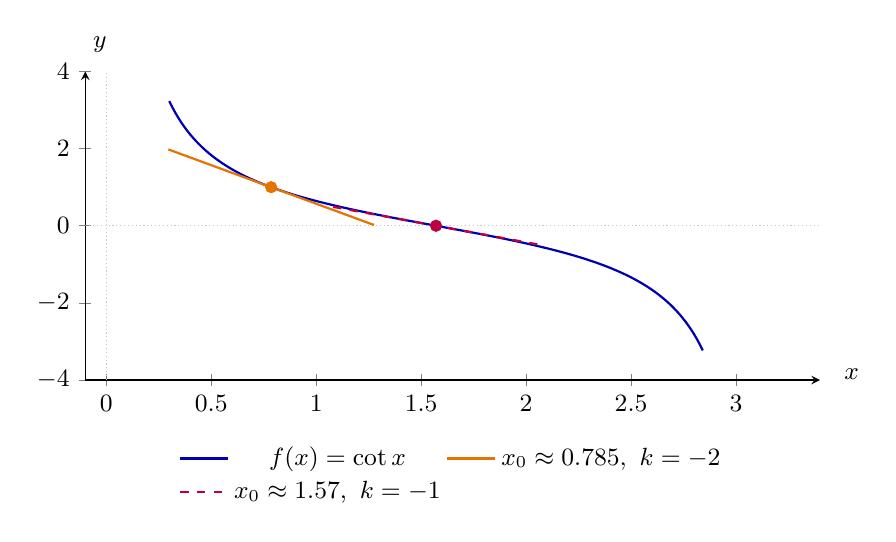
\begin{tikzpicture}[font=\small,>=stealth]
\begin{axis}[width=.90\linewidth,height=5.5cm,xmin=-0.1,xmax=3.4,ymin=-4,ymax=4,
axis lines=left,xlabel={$x$},ylabel={$y$},font=\small,
xlabel style={at={(axis description cs:1.02,.02)},anchor=west},
ylabel style={rotate=-90,at={(axis description cs:.02,1.03)},anchor=south},
legend style={at={(axis description cs:.5,-.18)},anchor=north,draw=none,fill=none,font=\small,legend columns=2},
unbounded coords=jump,clip=true,]
\addplot[gray!45,thin,densely dotted,forget plot] coordinates {(-0.1,0) (3.4,0)};
\addplot[gray!45,thin,densely dotted,forget plot] coordinates {(0,-4) (0,4)};
\addplot[blue!70!black,thick] coordinates {(0.3,3.2327281) (0.31411996,3.0780952) (0.32823992,2.9363447) (0.34235988,2.8058813) (0.35647984,2.6853621) (0.3705998,2.5736492) (0.38471976,2.4697712) (0.39883971,2.3728947) (0.41295967,2.2822999) (0.42707963,2.1973621) (0.44119959,2.1175368) (0.45531955,2.0423466) (0.46943951,1.9713718) (0.48355947,1.9042415) (0.49767943,1.8406269) (0.51179939,1.7802353) (0.52591935,1.7228057) (0.54003931,1.6681039) (0.55415927,1.6159198) (0.56827922,1.5660641) (0.58239918,1.5183657) (0.59651914,1.4726697) (0.6106391,1.4288356) (0.62475906,1.3867353) (0.63887902,1.3462522) (0.65299898,1.3072795) (0.66711894,1.2697196) (0.6812389,1.2334829) (0.69535886,1.1984869) (0.70947882,1.1646557) (0.72359878,1.1319193) (0.73771873,1.1002129) (0.75183869,1.0694766) (0.76595865,1.0396549) (0.78007861,1.0106961) (0.79419857,0.98255228) (0.80831853,0.95517874) (0.82243849,0.92853379) (0.83655845,0.90257853) (0.85067841,0.87727655) (0.86479837,0.85259378) (0.87891833,0.82849827) (0.89303829,0.80496003) (0.90715825,0.78195088) (0.9212782,0.75944432) (0.93539816,0.73741535) (0.94951812,0.71584043) (0.96363808,0.69469732) (0.97775804,0.67396499) (0.991878,0.65362357) (1.005998,0.6336542) (1.0201179,0.61403902) (1.0342379,0.59476108) (1.0483578,0.57580426) (1.0624778,0.55715322) (1.0765978,0.53879336) (1.0907177,0.52071077) (1.1048377,0.50289215) (1.1189576,0.48532482) (1.1330776,0.46799664) (1.1471976,0.45089598) (1.1613175,0.43401171) (1.1754375,0.41733313) (1.1895574,0.40084997) (1.2036774,0.38455237) (1.2177973,0.36843081) (1.2319173,0.35247613) (1.2460373,0.33667948) (1.2601572,0.32103233) (1.2742772,0.3055264) (1.2883971,0.29015369) (1.3025171,0.27490644) (1.3166371,0.2597771) (1.330757,0.24475836) (1.344877,0.22984308) (1.3589969,0.2150243) (1.3731169,0.20029524) (1.3872369,0.18564926) (1.4013568,0.17107987) (1.4154768,0.15658071) (1.4295967,0.14214552) (1.4437167,0.12776816) (1.4578367,0.11344259) (1.4719566,0.099162842) (1.4860766,0.084923029) (1.5001965,0.070717328) (1.5143165,0.05653997) (1.5284364,0.042385232) (1.5425564,0.028247428) (1.5566764,0.014120898) (1.5707963,-1.6081226e-16) (1.5849163,-0.014120898) (1.5990362,-0.028247428) (1.6131562,-0.042385232) (1.6272762,-0.05653997) (1.6413961,-0.070717328) (1.6555161,-0.084923029) (1.669636,-0.099162842) (1.683756,-0.11344259) (1.697876,-0.12776816) (1.7119959,-0.14214552) (1.7261159,-0.15658071) (1.7402358,-0.17107987) (1.7543558,-0.18564926) (1.7684758,-0.20029524) (1.7825957,-0.2150243) (1.7967157,-0.22984308) (1.8108356,-0.24475836) (1.8249556,-0.2597771) (1.8390756,-0.27490644) (1.8531955,-0.29015369) (1.8673155,-0.3055264) (1.8814354,-0.32103233) (1.8955554,-0.33667948) (1.9096753,-0.35247613) (1.9237953,-0.36843081) (1.9379153,-0.38455237) (1.9520352,-0.40084997) (1.9661552,-0.41733313) (1.9802751,-0.43401171) (1.9943951,-0.45089598) (2.0085151,-0.46799664) (2.022635,-0.48532482) (2.036755,-0.50289215) (2.0508749,-0.52071077) (2.0649949,-0.53879336) (2.0791149,-0.55715322) (2.0932348,-0.57580426) (2.1073548,-0.59476108) (2.1214747,-0.61403902) (2.1355947,-0.6336542) (2.1497147,-0.65362357) (2.1638346,-0.67396499) (2.1779546,-0.69469732) (2.1920745,-0.71584043) (2.2061945,-0.73741535) (2.2203144,-0.75944432) (2.2344344,-0.78195088) (2.2485544,-0.80496003) (2.2626743,-0.82849827) (2.2767943,-0.85259378) (2.2909142,-0.87727655) (2.3050342,-0.90257853) (2.3191542,-0.92853379) (2.3332741,-0.95517874) (2.3473941,-0.98255228) (2.361514,-1.0106961) (2.375634,-1.0396549) (2.389754,-1.0694766) (2.4038739,-1.1002129) (2.4179939,-1.1319193) (2.4321138,-1.1646557) (2.4462338,-1.1984869) (2.4603538,-1.2334829) (2.4744737,-1.2697196) (2.4885937,-1.3072795) (2.5027136,-1.3462522) (2.5168336,-1.3867353) (2.5309536,-1.4288356) (2.5450735,-1.4726697) (2.5591935,-1.5183657) (2.5733134,-1.5660641) (2.5874334,-1.6159198) (2.6015533,-1.6681039) (2.6156733,-1.7228057) (2.6297933,-1.7802353) (2.6439132,-1.8406269) (2.6580332,-1.9042415) (2.6721531,-1.9713718) (2.6862731,-2.0423466) (2.7003931,-2.1175368) (2.714513,-2.1973621) (2.728633,-2.2822999) (2.7427529,-2.3728947) (2.7568729,-2.4697712) (2.7709929,-2.5736492) (2.7851128,-2.6853621) (2.7992328,-2.8058813) (2.8133527,-2.9363447) (2.8274727,-3.0780952) (2.8415927,-3.2327281)};
\addlegendentry{$f(x)=\cot x$}
\addplot[orange!90!black,thick] coordinates {(0.29539816,1.98) (1.2753982,0.02)};
\addlegendentry{$x_0\approx0.785,\ k=-2$}
\addplot[only marks,mark=*,orange!90!black,forget plot] coordinates {(0.78539816,1)};
\addplot[purple,thick,dashed] coordinates {(1.0807963,0.49) (2.0607963,-0.49)};
\addlegendentry{$x_0\approx1.57,\ k=-1$}
\addplot[only marks,mark=*,purple,forget plot] coordinates {(1.5707963,6.123234e-17)};

\end{axis}
\end{tikzpicture}
\par\smallskip{\small $\sin x\ne0$；图中只画 $(0,\pi)$ 内的一段。}
\end{center}

\end{minipage}
\end{statementbox}

\begin{statementbox}
\begin{minipage}{\linewidth}
\textbf{结论16：正割}
\[
(\sec x)'=\sec x\tan x
\]
% F049: native TikZ/PGFPlots, computed from the stated mathematical model.
\begin{center}
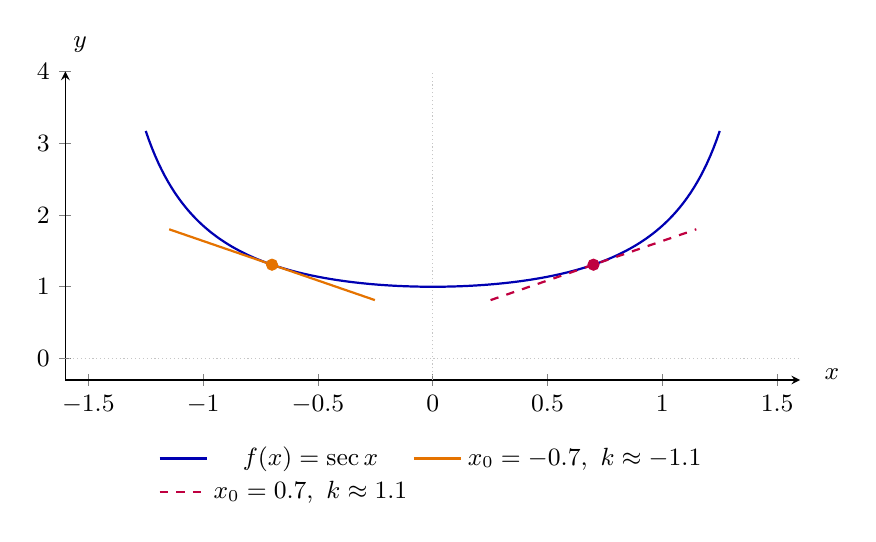
\begin{tikzpicture}[font=\small,>=stealth]
\begin{axis}[width=.90\linewidth,height=5.5cm,xmin=-1.6,xmax=1.6,ymin=-0.3,ymax=4,
axis lines=left,xlabel={$x$},ylabel={$y$},font=\small,
xlabel style={at={(axis description cs:1.02,.02)},anchor=west},
ylabel style={rotate=-90,at={(axis description cs:.02,1.03)},anchor=south},
legend style={at={(axis description cs:.5,-.18)},anchor=north,draw=none,fill=none,font=\small,legend columns=2},
unbounded coords=jump,clip=true,]
\addplot[gray!45,thin,densely dotted,forget plot] coordinates {(-1.6,0) (1.6,0)};
\addplot[gray!45,thin,densely dotted,forget plot] coordinates {(0,-0.3) (0,4)};
\addplot[blue!70!black,thick] coordinates {(-1.25,3.1713577) (-1.2361111,3.0444007) (-1.2222222,2.9277603) (-1.2083333,2.8202518) (-1.1944444,2.7208654) (-1.1805556,2.6287351) (-1.1666667,2.5431142) (-1.1527778,2.4633551) (-1.1388889,2.3888935) (-1.125,2.3192358) (-1.1111111,2.2539477) (-1.0972222,2.1926461) (-1.0833333,2.1349917) (-1.0694444,2.0806827) (-1.0555556,2.0294498) (-1.0416667,1.9810524) (-1.0277778,1.9352741) (-1.0138889,1.8919204) (-1,1.8508157) (-0.98611111,1.8118013) (-0.97222222,1.7747329) (-0.95833333,1.7394798) (-0.94444444,1.7059226) (-0.93055556,1.6739524) (-0.91666667,1.6434697) (-0.90277778,1.6143831) (-0.88888889,1.5866089) (-0.875,1.56007) (-0.86111111,1.5346956) (-0.84722222,1.51042) (-0.83333333,1.4871829) (-0.81944444,1.4649282) (-0.80555556,1.4436042) (-0.79166667,1.4231626) (-0.77777778,1.4035588) (-0.76388889,1.3847512) (-0.75,1.3667011) (-0.73611111,1.3493725) (-0.72222222,1.3327317) (-0.70833333,1.3167472) (-0.69444444,1.3013897) (-0.68055556,1.2866316) (-0.66666667,1.2724471) (-0.65277778,1.2588122) (-0.63888889,1.2457042) (-0.625,1.2331017) (-0.61111111,1.2209848) (-0.59722222,1.2093348) (-0.58333333,1.1981339) (-0.56944444,1.1873655) (-0.55555556,1.177014) (-0.54166667,1.1670646) (-0.52777778,1.1575034) (-0.51388889,1.1483173) (-0.5,1.1394939) (-0.48611111,1.1310216) (-0.47222222,1.1228894) (-0.45833333,1.1150868) (-0.44444444,1.1076041) (-0.43055556,1.100432) (-0.41666667,1.0935618) (-0.40277778,1.0869852) (-0.38888889,1.0806945) (-0.375,1.0746822) (-0.36111111,1.0689416) (-0.34722222,1.063466) (-0.33333333,1.0582493) (-0.31944444,1.0532857) (-0.30555556,1.0485698) (-0.29166667,1.0440964) (-0.27777778,1.0398608) (-0.26388889,1.0358584) (-0.25,1.032085) (-0.23611111,1.0285367) (-0.22222222,1.0252098) (-0.20833333,1.0221009) (-0.19444444,1.0192068) (-0.18055556,1.0165245) (-0.16666667,1.0140515) (-0.15277778,1.0117851) (-0.13888889,1.0097232) (-0.125,1.0078637) (-0.11111111,1.0062048) (-0.097222222,1.0047448) (-0.083333333,1.0034823) (-0.069444444,1.0024161) (-0.055555556,1.0015452) (-0.041666667,1.0008687) (-0.027777778,1.0003859) (-0.013888889,1.0000965) (0,1) (0.013888889,1.0000965) (0.027777778,1.0003859) (0.041666667,1.0008687) (0.055555556,1.0015452) (0.069444444,1.0024161) (0.083333333,1.0034823) (0.097222222,1.0047448) (0.11111111,1.0062048) (0.125,1.0078637) (0.13888889,1.0097232) (0.15277778,1.0117851) (0.16666667,1.0140515) (0.18055556,1.0165245) (0.19444444,1.0192068) (0.20833333,1.0221009) (0.22222222,1.0252098) (0.23611111,1.0285367) (0.25,1.032085) (0.26388889,1.0358584) (0.27777778,1.0398608) (0.29166667,1.0440964) (0.30555556,1.0485698) (0.31944444,1.0532857) (0.33333333,1.0582493) (0.34722222,1.063466) (0.36111111,1.0689416) (0.375,1.0746822) (0.38888889,1.0806945) (0.40277778,1.0869852) (0.41666667,1.0935618) (0.43055556,1.100432) (0.44444444,1.1076041) (0.45833333,1.1150868) (0.47222222,1.1228894) (0.48611111,1.1310216) (0.5,1.1394939) (0.51388889,1.1483173) (0.52777778,1.1575034) (0.54166667,1.1670646) (0.55555556,1.177014) (0.56944444,1.1873655) (0.58333333,1.1981339) (0.59722222,1.2093348) (0.61111111,1.2209848) (0.625,1.2331017) (0.63888889,1.2457042) (0.65277778,1.2588122) (0.66666667,1.2724471) (0.68055556,1.2866316) (0.69444444,1.3013897) (0.70833333,1.3167472) (0.72222222,1.3327317) (0.73611111,1.3493725) (0.75,1.3667011) (0.76388889,1.3847512) (0.77777778,1.4035588) (0.79166667,1.4231626) (0.80555556,1.4436042) (0.81944444,1.4649282) (0.83333333,1.4871829) (0.84722222,1.51042) (0.86111111,1.5346956) (0.875,1.56007) (0.88888889,1.5866089) (0.90277778,1.6143831) (0.91666667,1.6434697) (0.93055556,1.6739524) (0.94444444,1.7059226) (0.95833333,1.7394798) (0.97222222,1.7747329) (0.98611111,1.8118013) (1,1.8508157) (1.0138889,1.8919204) (1.0277778,1.9352741) (1.0416667,1.9810524) (1.0555556,2.0294498) (1.0694444,2.0806827) (1.0833333,2.1349917) (1.0972222,2.1926461) (1.1111111,2.2539477) (1.125,2.3192358) (1.1388889,2.3888935) (1.1527778,2.4633551) (1.1666667,2.5431142) (1.1805556,2.6287351) (1.1944444,2.7208654) (1.2083333,2.8202518) (1.2222222,2.9277603) (1.2361111,3.0444007) (1.25,3.1713577)};
\addlegendentry{$f(x)=\sec x$}
\addplot[orange!90!black,thick] coordinates {(-1.148,1.8008227) (-0.252,0.81409579)};
\addlegendentry{$x_0=-0.7,\ k\approx-1.1$}
\addplot[only marks,mark=*,orange!90!black,forget plot] coordinates {(-0.7,1.3074593)};
\addplot[purple,thick,dashed] coordinates {(0.252,0.81409579) (1.148,1.8008227)};
\addlegendentry{$x_0=0.7,\ k\approx1.1$}
\addplot[only marks,mark=*,purple,forget plot] coordinates {(0.7,1.3074593)};

\end{axis}
\end{tikzpicture}
\par\smallskip{\small $\cos x\ne0$；左右两侧切线斜率分别为负、正。}
\end{center}

\end{minipage}
记号：$\sec x=1/\cos x$，$\csc x=1/\sin x$，$\cot x=\cos x/\sin x$。
\end{statementbox}

\begin{statementbox}
\begin{minipage}{\linewidth}
\textbf{结论17：余割}
\[
(\csc x)'=-\csc x\cot x
\]
% F049: native TikZ/PGFPlots, computed from the stated mathematical model.
\begin{center}
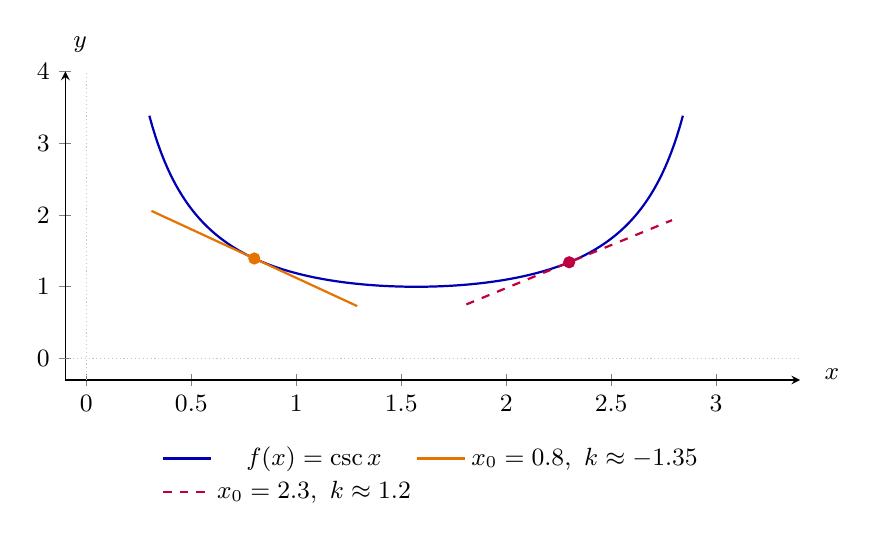
\begin{tikzpicture}[font=\small,>=stealth]
\begin{axis}[width=.90\linewidth,height=5.5cm,xmin=-0.1,xmax=3.4,ymin=-0.3,ymax=4,
axis lines=left,xlabel={$x$},ylabel={$y$},font=\small,
xlabel style={at={(axis description cs:1.02,.02)},anchor=west},
ylabel style={rotate=-90,at={(axis description cs:.02,1.03)},anchor=south},
legend style={at={(axis description cs:.5,-.18)},anchor=north,draw=none,fill=none,font=\small,legend columns=2},
unbounded coords=jump,clip=true,]
\addplot[gray!45,thin,densely dotted,forget plot] coordinates {(-0.1,0) (3.4,0)};
\addplot[gray!45,thin,densely dotted,forget plot] coordinates {(0,-0.3) (0,4)};
\addplot[blue!70!black,thick] coordinates {(0.3,3.3838634) (0.31411996,3.2364595) (0.32823992,3.1019543) (0.34235988,2.978753) (0.35647984,2.8655139) (0.3705998,2.7610994) (0.38471976,2.6645394) (0.39883971,2.5750008) (0.41295967,2.491765) (0.42707963,2.414208) (0.44119959,2.3417861) (0.45531955,2.2740228) (0.46943951,2.2104992) (0.48355947,2.1508453) (0.49767943,2.0947332) (0.51179939,2.0418712) (0.52591935,1.9919988) (0.54003931,1.9448832) (0.55415927,1.9003149) (0.56827922,1.8581057) (0.58239918,1.8180853) (0.59651914,1.7801) (0.6106391,1.7440101) (0.62475906,1.7096885) (0.63887902,1.6770197) (0.65299898,1.6458979) (0.66711894,1.6162265) (0.6812389,1.5879169) (0.69535886,1.5608878) (0.70947882,1.5350645) (0.72359878,1.5103779) (0.73771873,1.4867644) (0.75183869,1.4641654) (0.76595865,1.4425264) (0.78007861,1.421797) (0.79419857,1.4019304) (0.80831853,1.3828834) (0.82243849,1.3646153) (0.83655845,1.3470887) (0.85067841,1.3302684) (0.86479837,1.3141218) (0.87891833,1.2986183) (0.89303829,1.2837292) (0.90715825,1.2694279) (0.9212782,1.2556893) (0.93539816,1.24249) (0.94951812,1.2298079) (0.96363808,1.2176224) (0.97775804,1.2059141) (0.991878,1.1946647) (1.005998,1.1838571) (1.0201179,1.1734751) (1.0342379,1.1635036) (1.0483578,1.1539283) (1.0624778,1.1447356) (1.0765978,1.135913) (1.0907177,1.1274483) (1.1048377,1.1193304) (1.1189576,1.1115486) (1.1330776,1.1040928) (1.1471976,1.0969536) (1.1613175,1.0901221) (1.1754375,1.0835898) (1.1895574,1.0773489) (1.2036774,1.0713919) (1.2177973,1.0657116) (1.2319173,1.0603016) (1.2460373,1.0551555) (1.2601572,1.0502675) (1.2742772,1.045632) (1.2883971,1.041244) (1.3025171,1.0370986) (1.3166371,1.0331912) (1.330757,1.0295177) (1.344877,1.026074) (1.3589969,1.0228565) (1.3731169,1.0198618) (1.3872369,1.0170868) (1.4013568,1.0145286) (1.4154768,1.0121845) (1.4295967,1.0100522) (1.4437167,1.0081293) (1.4578367,1.006414) (1.4719566,1.0049046) (1.4860766,1.0035995) (1.5001965,1.0024974) (1.5143165,1.0015971) (1.5284364,1.0008979) (1.5425564,1.0003989) (1.5566764,1.0000997) (1.5707963,1) (1.5849163,1.0000997) (1.5990362,1.0003989) (1.6131562,1.0008979) (1.6272762,1.0015971) (1.6413961,1.0024974) (1.6555161,1.0035995) (1.669636,1.0049046) (1.683756,1.006414) (1.697876,1.0081293) (1.7119959,1.0100522) (1.7261159,1.0121845) (1.7402358,1.0145286) (1.7543558,1.0170868) (1.7684758,1.0198618) (1.7825957,1.0228565) (1.7967157,1.026074) (1.8108356,1.0295177) (1.8249556,1.0331912) (1.8390756,1.0370986) (1.8531955,1.041244) (1.8673155,1.045632) (1.8814354,1.0502675) (1.8955554,1.0551555) (1.9096753,1.0603016) (1.9237953,1.0657116) (1.9379153,1.0713919) (1.9520352,1.0773489) (1.9661552,1.0835898) (1.9802751,1.0901221) (1.9943951,1.0969536) (2.0085151,1.1040928) (2.022635,1.1115486) (2.036755,1.1193304) (2.0508749,1.1274483) (2.0649949,1.135913) (2.0791149,1.1447356) (2.0932348,1.1539283) (2.1073548,1.1635036) (2.1214747,1.1734751) (2.1355947,1.1838571) (2.1497147,1.1946647) (2.1638346,1.2059141) (2.1779546,1.2176224) (2.1920745,1.2298079) (2.2061945,1.24249) (2.2203144,1.2556893) (2.2344344,1.2694279) (2.2485544,1.2837292) (2.2626743,1.2986183) (2.2767943,1.3141218) (2.2909142,1.3302684) (2.3050342,1.3470887) (2.3191542,1.3646153) (2.3332741,1.3828834) (2.3473941,1.4019304) (2.361514,1.421797) (2.375634,1.4425264) (2.389754,1.4641654) (2.4038739,1.4867644) (2.4179939,1.5103779) (2.4321138,1.5350645) (2.4462338,1.5608878) (2.4603538,1.5879169) (2.4744737,1.6162265) (2.4885937,1.6458979) (2.5027136,1.6770197) (2.5168336,1.7096885) (2.5309536,1.7440101) (2.5450735,1.7801) (2.5591935,1.8180853) (2.5733134,1.8581057) (2.5874334,1.9003149) (2.6015533,1.9448832) (2.6156733,1.9919988) (2.6297933,2.0418712) (2.6439132,2.0947332) (2.6580332,2.1508453) (2.6721531,2.2104992) (2.6862731,2.2740228) (2.7003931,2.3417861) (2.714513,2.414208) (2.728633,2.491765) (2.7427529,2.5750008) (2.7568729,2.6645394) (2.7709929,2.7610994) (2.7851128,2.8655139) (2.7992328,2.978753) (2.8133527,3.1019543) (2.8274727,3.2364595) (2.8415927,3.3838634)};
\addlegendentry{$f(x)=\csc x$}
\addplot[orange!90!black,thick] coordinates {(0.31,2.0574094) (1.29,0.73060625)};
\addlegendentry{$x_0=0.8,\ k\approx-1.35$}
\addplot[only marks,mark=*,orange!90!black,forget plot] coordinates {(0.8,1.3940078)};
\addplot[purple,thick,dashed] coordinates {(1.81,0.75390731) (2.79,1.9281177)};
\addlegendentry{$x_0=2.3,\ k\approx1.2$}
\addplot[only marks,mark=*,purple,forget plot] coordinates {(2.3,1.3410125)};

\end{axis}
\end{tikzpicture}
\par\smallskip{\small $\sin x\ne0$；最低点 $x=\pi/2$ 处斜率为零。}
\end{center}

\end{minipage}
\end{statementbox}

\begin{statementbox}
\begin{minipage}{\linewidth}
\textbf{结论18：绝对值}
\[
(|x|)'=\begin{cases}1,&x>0,\\-1,&x<0.\end{cases}
\]
% F049: native TikZ/PGFPlots, computed from the stated mathematical model.
\begin{center}
\begin{tikzpicture}[font=\small,>=stealth]
\begin{axis}[width=.90\linewidth,height=5.5cm,xmin=-2.3,xmax=2.3,ymin=-0.4,ymax=2.6,
axis lines=left,xlabel={$x$},ylabel={$y$},font=\small,
xlabel style={at={(axis description cs:1.02,.02)},anchor=west},
ylabel style={rotate=-90,at={(axis description cs:.02,1.03)},anchor=south},
legend style={at={(axis description cs:.5,-.18)},anchor=north,draw=none,fill=none,font=\small,legend columns=2},
unbounded coords=jump,clip=true,]
\addplot[gray!45,thin,densely dotted,forget plot] coordinates {(-2.3,0) (2.3,0)};
\addplot[gray!45,thin,densely dotted,forget plot] coordinates {(0,-0.4) (0,2.6)};
\addplot[blue!70!black,thick] coordinates {(-2,2) (-1.9888889,1.9888889) (-1.9777778,1.9777778) (-1.9666667,1.9666667) (-1.9555556,1.9555556) (-1.9444444,1.9444444) (-1.9333333,1.9333333) (-1.9222222,1.9222222) (-1.9111111,1.9111111) (-1.9,1.9) (-1.8888889,1.8888889) (-1.8777778,1.8777778) (-1.8666667,1.8666667) (-1.8555556,1.8555556) (-1.8444444,1.8444444) (-1.8333333,1.8333333) (-1.8222222,1.8222222) (-1.8111111,1.8111111) (-1.8,1.8) (-1.7888889,1.7888889) (-1.7777778,1.7777778) (-1.7666667,1.7666667) (-1.7555556,1.7555556) (-1.7444444,1.7444444) (-1.7333333,1.7333333) (-1.7222222,1.7222222) (-1.7111111,1.7111111) (-1.7,1.7) (-1.6888889,1.6888889) (-1.6777778,1.6777778) (-1.6666667,1.6666667) (-1.6555556,1.6555556) (-1.6444444,1.6444444) (-1.6333333,1.6333333) (-1.6222222,1.6222222) (-1.6111111,1.6111111) (-1.6,1.6) (-1.5888889,1.5888889) (-1.5777778,1.5777778) (-1.5666667,1.5666667) (-1.5555556,1.5555556) (-1.5444444,1.5444444) (-1.5333333,1.5333333) (-1.5222222,1.5222222) (-1.5111111,1.5111111) (-1.5,1.5) (-1.4888889,1.4888889) (-1.4777778,1.4777778) (-1.4666667,1.4666667) (-1.4555556,1.4555556) (-1.4444444,1.4444444) (-1.4333333,1.4333333) (-1.4222222,1.4222222) (-1.4111111,1.4111111) (-1.4,1.4) (-1.3888889,1.3888889) (-1.3777778,1.3777778) (-1.3666667,1.3666667) (-1.3555556,1.3555556) (-1.3444444,1.3444444) (-1.3333333,1.3333333) (-1.3222222,1.3222222) (-1.3111111,1.3111111) (-1.3,1.3) (-1.2888889,1.2888889) (-1.2777778,1.2777778) (-1.2666667,1.2666667) (-1.2555556,1.2555556) (-1.2444444,1.2444444) (-1.2333333,1.2333333) (-1.2222222,1.2222222) (-1.2111111,1.2111111) (-1.2,1.2) (-1.1888889,1.1888889) (-1.1777778,1.1777778) (-1.1666667,1.1666667) (-1.1555556,1.1555556) (-1.1444444,1.1444444) (-1.1333333,1.1333333) (-1.1222222,1.1222222) (-1.1111111,1.1111111) (-1.1,1.1) (-1.0888889,1.0888889) (-1.0777778,1.0777778) (-1.0666667,1.0666667) (-1.0555556,1.0555556) (-1.0444444,1.0444444) (-1.0333333,1.0333333) (-1.0222222,1.0222222) (-1.0111111,1.0111111) (-1,1) (-0.98888889,0.98888889) (-0.97777778,0.97777778) (-0.96666667,0.96666667) (-0.95555556,0.95555556) (-0.94444444,0.94444444) (-0.93333333,0.93333333) (-0.92222222,0.92222222) (-0.91111111,0.91111111) (-0.9,0.9) (-0.88888889,0.88888889) (-0.87777778,0.87777778) (-0.86666667,0.86666667) (-0.85555556,0.85555556) (-0.84444444,0.84444444) (-0.83333333,0.83333333) (-0.82222222,0.82222222) (-0.81111111,0.81111111) (-0.8,0.8) (-0.78888889,0.78888889) (-0.77777778,0.77777778) (-0.76666667,0.76666667) (-0.75555556,0.75555556) (-0.74444444,0.74444444) (-0.73333333,0.73333333) (-0.72222222,0.72222222) (-0.71111111,0.71111111) (-0.7,0.7) (-0.68888889,0.68888889) (-0.67777778,0.67777778) (-0.66666667,0.66666667) (-0.65555556,0.65555556) (-0.64444444,0.64444444) (-0.63333333,0.63333333) (-0.62222222,0.62222222) (-0.61111111,0.61111111) (-0.6,0.6) (-0.58888889,0.58888889) (-0.57777778,0.57777778) (-0.56666667,0.56666667) (-0.55555556,0.55555556) (-0.54444444,0.54444444) (-0.53333333,0.53333333) (-0.52222222,0.52222222) (-0.51111111,0.51111111) (-0.5,0.5) (-0.48888889,0.48888889) (-0.47777778,0.47777778) (-0.46666667,0.46666667) (-0.45555556,0.45555556) (-0.44444444,0.44444444) (-0.43333333,0.43333333) (-0.42222222,0.42222222) (-0.41111111,0.41111111) (-0.4,0.4) (-0.38888889,0.38888889) (-0.37777778,0.37777778) (-0.36666667,0.36666667) (-0.35555556,0.35555556) (-0.34444444,0.34444444) (-0.33333333,0.33333333) (-0.32222222,0.32222222) (-0.31111111,0.31111111) (-0.3,0.3) (-0.28888889,0.28888889) (-0.27777778,0.27777778) (-0.26666667,0.26666667) (-0.25555556,0.25555556) (-0.24444444,0.24444444) (-0.23333333,0.23333333) (-0.22222222,0.22222222) (-0.21111111,0.21111111) (-0.2,0.2) (-0.18888889,0.18888889) (-0.17777778,0.17777778) (-0.16666667,0.16666667) (-0.15555556,0.15555556) (-0.14444444,0.14444444) (-0.13333333,0.13333333) (-0.12222222,0.12222222) (-0.11111111,0.11111111) (-0.1,0.1) (-0.088888889,0.088888889) (-0.077777778,0.077777778) (-0.066666667,0.066666667) (-0.055555556,0.055555556) (-0.044444444,0.044444444) (-0.033333333,0.033333333) (-0.022222222,0.022222222) (-0.011111111,0.011111111) (0,0)};
\addlegendentry{$f(x)=|x|$}
\addplot[blue!70!black,thick,forget plot] coordinates {(0,0) (0.011111111,0.011111111) (0.022222222,0.022222222) (0.033333333,0.033333333) (0.044444444,0.044444444) (0.055555556,0.055555556) (0.066666667,0.066666667) (0.077777778,0.077777778) (0.088888889,0.088888889) (0.1,0.1) (0.11111111,0.11111111) (0.12222222,0.12222222) (0.13333333,0.13333333) (0.14444444,0.14444444) (0.15555556,0.15555556) (0.16666667,0.16666667) (0.17777778,0.17777778) (0.18888889,0.18888889) (0.2,0.2) (0.21111111,0.21111111) (0.22222222,0.22222222) (0.23333333,0.23333333) (0.24444444,0.24444444) (0.25555556,0.25555556) (0.26666667,0.26666667) (0.27777778,0.27777778) (0.28888889,0.28888889) (0.3,0.3) (0.31111111,0.31111111) (0.32222222,0.32222222) (0.33333333,0.33333333) (0.34444444,0.34444444) (0.35555556,0.35555556) (0.36666667,0.36666667) (0.37777778,0.37777778) (0.38888889,0.38888889) (0.4,0.4) (0.41111111,0.41111111) (0.42222222,0.42222222) (0.43333333,0.43333333) (0.44444444,0.44444444) (0.45555556,0.45555556) (0.46666667,0.46666667) (0.47777778,0.47777778) (0.48888889,0.48888889) (0.5,0.5) (0.51111111,0.51111111) (0.52222222,0.52222222) (0.53333333,0.53333333) (0.54444444,0.54444444) (0.55555556,0.55555556) (0.56666667,0.56666667) (0.57777778,0.57777778) (0.58888889,0.58888889) (0.6,0.6) (0.61111111,0.61111111) (0.62222222,0.62222222) (0.63333333,0.63333333) (0.64444444,0.64444444) (0.65555556,0.65555556) (0.66666667,0.66666667) (0.67777778,0.67777778) (0.68888889,0.68888889) (0.7,0.7) (0.71111111,0.71111111) (0.72222222,0.72222222) (0.73333333,0.73333333) (0.74444444,0.74444444) (0.75555556,0.75555556) (0.76666667,0.76666667) (0.77777778,0.77777778) (0.78888889,0.78888889) (0.8,0.8) (0.81111111,0.81111111) (0.82222222,0.82222222) (0.83333333,0.83333333) (0.84444444,0.84444444) (0.85555556,0.85555556) (0.86666667,0.86666667) (0.87777778,0.87777778) (0.88888889,0.88888889) (0.9,0.9) (0.91111111,0.91111111) (0.92222222,0.92222222) (0.93333333,0.93333333) (0.94444444,0.94444444) (0.95555556,0.95555556) (0.96666667,0.96666667) (0.97777778,0.97777778) (0.98888889,0.98888889) (1,1) (1.0111111,1.0111111) (1.0222222,1.0222222) (1.0333333,1.0333333) (1.0444444,1.0444444) (1.0555556,1.0555556) (1.0666667,1.0666667) (1.0777778,1.0777778) (1.0888889,1.0888889) (1.1,1.1) (1.1111111,1.1111111) (1.1222222,1.1222222) (1.1333333,1.1333333) (1.1444444,1.1444444) (1.1555556,1.1555556) (1.1666667,1.1666667) (1.1777778,1.1777778) (1.1888889,1.1888889) (1.2,1.2) (1.2111111,1.2111111) (1.2222222,1.2222222) (1.2333333,1.2333333) (1.2444444,1.2444444) (1.2555556,1.2555556) (1.2666667,1.2666667) (1.2777778,1.2777778) (1.2888889,1.2888889) (1.3,1.3) (1.3111111,1.3111111) (1.3222222,1.3222222) (1.3333333,1.3333333) (1.3444444,1.3444444) (1.3555556,1.3555556) (1.3666667,1.3666667) (1.3777778,1.3777778) (1.3888889,1.3888889) (1.4,1.4) (1.4111111,1.4111111) (1.4222222,1.4222222) (1.4333333,1.4333333) (1.4444444,1.4444444) (1.4555556,1.4555556) (1.4666667,1.4666667) (1.4777778,1.4777778) (1.4888889,1.4888889) (1.5,1.5) (1.5111111,1.5111111) (1.5222222,1.5222222) (1.5333333,1.5333333) (1.5444444,1.5444444) (1.5555556,1.5555556) (1.5666667,1.5666667) (1.5777778,1.5777778) (1.5888889,1.5888889) (1.6,1.6) (1.6111111,1.6111111) (1.6222222,1.6222222) (1.6333333,1.6333333) (1.6444444,1.6444444) (1.6555556,1.6555556) (1.6666667,1.6666667) (1.6777778,1.6777778) (1.6888889,1.6888889) (1.7,1.7) (1.7111111,1.7111111) (1.7222222,1.7222222) (1.7333333,1.7333333) (1.7444444,1.7444444) (1.7555556,1.7555556) (1.7666667,1.7666667) (1.7777778,1.7777778) (1.7888889,1.7888889) (1.8,1.8) (1.8111111,1.8111111) (1.8222222,1.8222222) (1.8333333,1.8333333) (1.8444444,1.8444444) (1.8555556,1.8555556) (1.8666667,1.8666667) (1.8777778,1.8777778) (1.8888889,1.8888889) (1.9,1.9) (1.9111111,1.9111111) (1.9222222,1.9222222) (1.9333333,1.9333333) (1.9444444,1.9444444) (1.9555556,1.9555556) (1.9666667,1.9666667) (1.9777778,1.9777778) (1.9888889,1.9888889) (2,2)};
\addplot[orange!90!black,thick] coordinates {(-1.644,1.644) (-0.356,0.356)};
\addlegendentry{$x_0=-1,\ k=-1$}
\addplot[only marks,mark=*,orange!90!black,forget plot] coordinates {(-1,1)};
\addplot[purple,thick,dashed] coordinates {(0.356,0.356) (1.644,1.644)};
\addlegendentry{$x_0=1,\ k=1$}
\addplot[only marks,mark=*,purple,forget plot] coordinates {(1,1)};

\end{axis}
\end{tikzpicture}
\par\smallskip{\small $x=0$ 左右斜率不同，所以不可导。}
\end{center}

\end{minipage}
\end{statementbox}

\begin{statementbox}
\begin{minipage}{\linewidth}
\textbf{结论19：变指数}
\[
(x^x)'=x^x(\ln x+1)
\]
% F049: native TikZ/PGFPlots, computed from the stated mathematical model.
\begin{center}
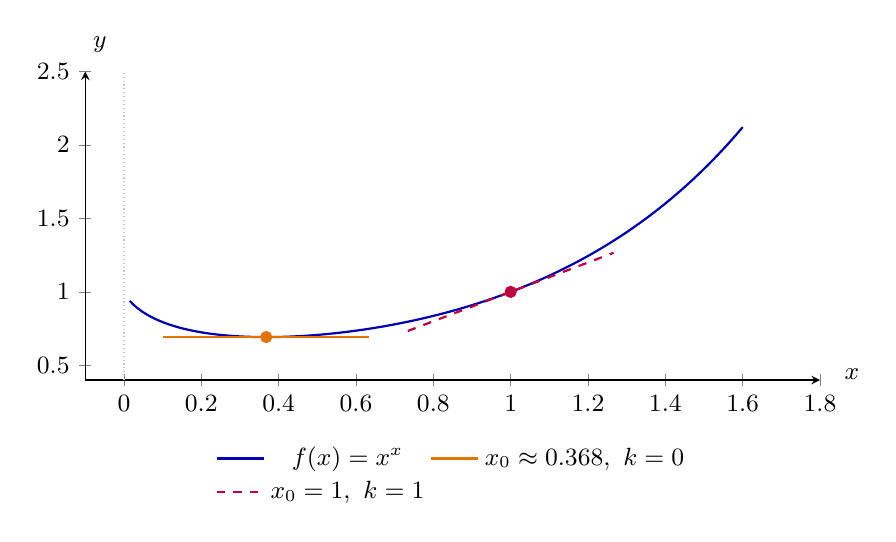
\begin{tikzpicture}[font=\small,>=stealth]
\begin{axis}[width=.90\linewidth,height=5.5cm,xmin=-0.1,xmax=1.8,ymin=0.4,ymax=2.5,
axis lines=left,xlabel={$x$},ylabel={$y$},font=\small,
xlabel style={at={(axis description cs:1.02,.02)},anchor=west},
ylabel style={rotate=-90,at={(axis description cs:.02,1.03)},anchor=south},
legend style={at={(axis description cs:.5,-.18)},anchor=north,draw=none,fill=none,font=\small,legend columns=2},
unbounded coords=jump,clip=true,]
\addplot[gray!45,thin,densely dotted,forget plot] coordinates {(0,0.4) (0,2.5)};
\addplot[blue!70!black,thick] coordinates {(0.015,0.93894763) (0.023805556,0.91486271) (0.032611111,0.89437407) (0.041416667,0.87645173) (0.050222222,0.86051037) (0.059027778,0.84617111) (0.067833333,0.8331686) (0.076638889,0.82130681) (0.085444444,0.81043524) (0.09425,0.8004349) (0.10305556,0.79120956) (0.11186111,0.78267992) (0.12066667,0.77477965) (0.12947222,0.76745255) (0.13827778,0.76065049) (0.14708333,0.75433187) (0.15588889,0.74846044) (0.16469444,0.74300438) (0.1735,0.7379356) (0.18230556,0.73322914) (0.19111111,0.72886275) (0.19991667,0.72481649) (0.20872222,0.72107239) (0.21752778,0.71761424) (0.22633333,0.71442737) (0.23513889,0.71149841) (0.24394444,0.70881521) (0.25275,0.70636666) (0.26155556,0.70414259) (0.27036111,0.70213368) (0.27916667,0.70033137) (0.28797222,0.69872775) (0.29677778,0.69731556) (0.30558333,0.6960881) (0.31438889,0.69503915) (0.32319444,0.69416299) (0.332,0.6934543) (0.34080556,0.69290816) (0.34961111,0.69252001) (0.35841667,0.69228561) (0.36722222,0.69220103) (0.37602778,0.69226264) (0.38483333,0.69246704) (0.39363889,0.69281108) (0.40244444,0.69329186) (0.41125,0.69390666) (0.42005556,0.69465298) (0.42886111,0.69552848) (0.43766667,0.69653101) (0.44647222,0.69765859) (0.45527778,0.69890937) (0.46408333,0.70028165) (0.47288889,0.70177388) (0.48169444,0.70338461) (0.4905,0.70511253) (0.49930556,0.70695646) (0.50811111,0.70891529) (0.51691667,0.71098804) (0.52572222,0.71317383) (0.53452778,0.71547186) (0.54333333,0.71788143) (0.55213889,0.72040191) (0.56094444,0.72303278) (0.56975,0.72577357) (0.57855556,0.72862391) (0.58736111,0.73158349) (0.59616667,0.73465207) (0.60497222,0.73782948) (0.61377778,0.74111561) (0.62258333,0.74451043) (0.63138889,0.74801396) (0.64019444,0.75162628) (0.649,0.75534752) (0.65780556,0.75917789) (0.66661111,0.76311762) (0.67541667,0.76716704) (0.68422222,0.77132649) (0.69302778,0.77559638) (0.70183333,0.77997717) (0.71063889,0.78446937) (0.71944444,0.78907353) (0.72825,0.79379027) (0.73705556,0.79862022) (0.74586111,0.8035641) (0.75466667,0.80862265) (0.76347222,0.81379664) (0.77227778,0.81908693) (0.78108333,0.82449439) (0.78988889,0.83001994) (0.79869444,0.83566455) (0.8075,0.84142923) (0.81630556,0.84731503) (0.82511111,0.85332306) (0.83391667,0.85945445) (0.84272222,0.86571039) (0.85152778,0.87209211) (0.86033333,0.87860087) (0.86913889,0.88523798) (0.87794444,0.89200481) (0.88675,0.89890276) (0.89555556,0.90593325) (0.90436111,0.91309779) (0.91316667,0.9203979) (0.92197222,0.92783516) (0.93077778,0.93541118) (0.93958333,0.94312762) (0.94838889,0.95098619) (0.95719444,0.95898865) (0.966,0.96713679) (0.97480556,0.97543245) (0.98361111,0.98387753) (0.99241667,0.99247396) (1.0012222,1.0012237) (1.0100278,1.0101288) (1.0188333,1.0191914) (1.0276389,1.0284135) (1.0364444,1.0377974) (1.04525,1.0473453) (1.0540556,1.0570594) (1.0628611,1.0669421) (1.0716667,1.0769958) (1.0804722,1.0872228) (1.0892778,1.0976258) (1.0980833,1.1082071) (1.1068889,1.1189695) (1.1156944,1.1299156) (1.1245,1.141048) (1.1333056,1.1523696) (1.1421111,1.1638831) (1.1509167,1.1755914) (1.1597222,1.1874976) (1.1685278,1.1996045) (1.1773333,1.2119153) (1.1861389,1.2244331) (1.1949444,1.237161) (1.20375,1.2501023) (1.2125556,1.2632604) (1.2213611,1.2766387) (1.2301667,1.2902405) (1.2389722,1.3040694) (1.2477778,1.318129) (1.2565833,1.332423) (1.2653889,1.3469551) (1.2741944,1.3617292) (1.283,1.3767491) (1.2918056,1.3920188) (1.3006111,1.4075423) (1.3094167,1.4233238) (1.3182222,1.4393674) (1.3270278,1.4556776) (1.3358333,1.4722585) (1.3446389,1.4891148) (1.3534444,1.5062509) (1.36225,1.5236715) (1.3710556,1.5413813) (1.3798611,1.5593852) (1.3886667,1.5776879) (1.3974722,1.5962947) (1.4062778,1.6152105) (1.4150833,1.6344405) (1.4238889,1.6539901) (1.4326944,1.6738647) (1.4415,1.6940699) (1.4503056,1.7146111) (1.4591111,1.7354942) (1.4679167,1.7567249) (1.4767222,1.7783094) (1.4855278,1.8002535) (1.4943333,1.8225636) (1.5031389,1.8452459) (1.5119444,1.8683069) (1.52075,1.891753) (1.5295556,1.9155911) (1.5383611,1.9398279) (1.5471667,1.9644704) (1.5559722,1.9895256) (1.5647778,2.0150008) (1.5735833,2.0409033) (1.5823889,2.0672406) (1.5911944,2.0940205) (1.6,2.1212506)};
\addlegendentry{$f(x)=x^x$}
\addplot[orange!90!black,thick] coordinates {(0.10187944,0.69220063) (0.63387944,0.69220063)};
\addlegendentry{$x_0\approx0.368,\ k=0$}
\addplot[only marks,mark=*,orange!90!black,forget plot] coordinates {(0.36787944,0.69220063)};
\addplot[purple,thick,dashed] coordinates {(0.734,0.734) (1.266,1.266)};
\addlegendentry{$x_0=1,\ k=1$}
\addplot[only marks,mark=*,purple,forget plot] coordinates {(1,1)};

\end{axis}
\end{tikzpicture}
\par\smallskip{\small $x>0$；在 $x=1/e$ 处由下降转为上升。}
\end{center}

\end{minipage}
\end{statementbox}

\begin{statementbox}
\begin{minipage}{\linewidth}
\textbf{结论20：反正弦（拓展）}
\[
(\arcsin x)'=1/\sqrt{1-x^2}
\]
% F049: native TikZ/PGFPlots, computed from the stated mathematical model.
\begin{center}
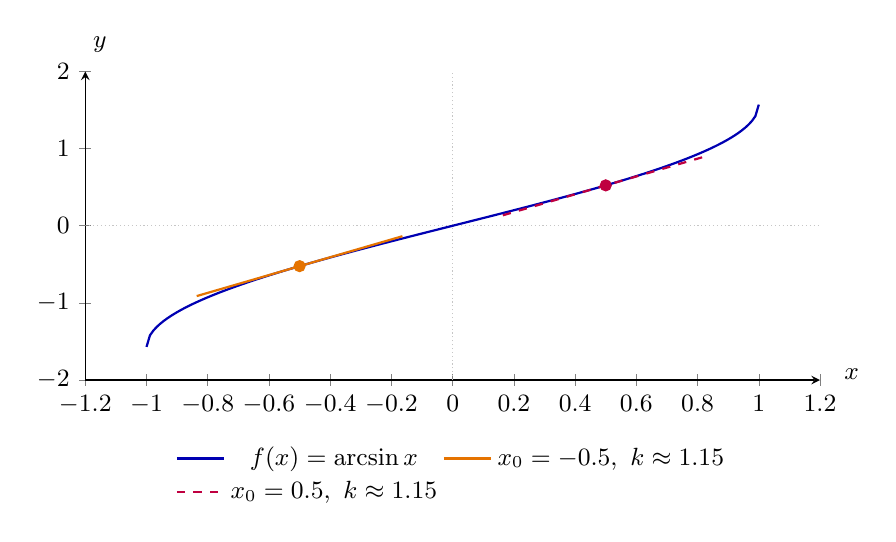
\begin{tikzpicture}[font=\small,>=stealth]
\begin{axis}[width=.90\linewidth,height=5.5cm,xmin=-1.2,xmax=1.2,ymin=-2,ymax=2,
axis lines=left,xlabel={$x$},ylabel={$y$},font=\small,
xlabel style={at={(axis description cs:1.02,.02)},anchor=west},
ylabel style={rotate=-90,at={(axis description cs:.02,1.03)},anchor=south},
legend style={at={(axis description cs:.5,-.18)},anchor=north,draw=none,fill=none,font=\small,legend columns=2},
unbounded coords=jump,clip=true,]
\addplot[gray!45,thin,densely dotted,forget plot] coordinates {(-1.2,0) (1.2,0)};
\addplot[gray!45,thin,densely dotted,forget plot] coordinates {(0,-2) (0,2)};
\addplot[blue!70!black,thick] coordinates {(-1,-1.5707963) (-0.98888889,-1.4215868) (-0.97777778,-1.3595854) (-0.96666667,-1.3118748) (-0.95555556,-1.2715385) (-0.94444444,-1.2359002) (-0.93333333,-1.2035883) (-0.92222222,-1.1737889) (-0.91111111,-1.1459719) (-0.9,-1.1197695) (-0.88888889,-1.0949141) (-0.87777778,-1.0712037) (-0.86666667,-1.0484815) (-0.85555556,-1.026623) (-0.84444444,-1.0055271) (-0.83333333,-0.98511078) (-0.82222222,-0.96530442) (-0.81111111,-0.94604931) (-0.8,-0.92729522) (-0.78888889,-0.90899884) (-0.77777778,-0.89112251) (-0.76666667,-0.87363319) (-0.75555556,-0.85650177) (-0.74444444,-0.83970239) (-0.73333333,-0.82321198) (-0.72222222,-0.80700983) (-0.71111111,-0.7910773) (-0.7,-0.7753975) (-0.68888889,-0.75995509) (-0.67777778,-0.74473607) (-0.66666667,-0.72972766) (-0.65555556,-0.71491808) (-0.64444444,-0.70029651) (-0.63333333,-0.68585296) (-0.62222222,-0.67157818) (-0.61111111,-0.65746356) (-0.6,-0.64350111) (-0.58888889,-0.62968338) (-0.57777778,-0.61600339) (-0.56666667,-0.60245463) (-0.55555556,-0.58903097) (-0.54444444,-0.57572665) (-0.53333333,-0.56253624) (-0.52222222,-0.54945464) (-0.51111111,-0.53647701) (-0.5,-0.52359878) (-0.48888889,-0.51081559) (-0.47777778,-0.49812335) (-0.46666667,-0.48551812) (-0.45555556,-0.47299619) (-0.44444444,-0.46055399) (-0.43333333,-0.44818814) (-0.42222222,-0.43589538) (-0.41111111,-0.42367261) (-0.4,-0.41151685) (-0.38888889,-0.39942524) (-0.37777778,-0.38739504) (-0.36666667,-0.37542361) (-0.35555556,-0.3635084) (-0.34444444,-0.35164695) (-0.33333333,-0.33983691) (-0.32222222,-0.32807598) (-0.31111111,-0.31636194) (-0.3,-0.30469265) (-0.28888889,-0.29306604) (-0.27777778,-0.28148007) (-0.26666667,-0.2699328) (-0.25555556,-0.2584223) (-0.24444444,-0.24694671) (-0.23333333,-0.23550424) (-0.22222222,-0.22409309) (-0.21111111,-0.21271155) (-0.2,-0.20135792) (-0.18888889,-0.19003054) (-0.17777778,-0.17872779) (-0.16666667,-0.16744808) (-0.15555556,-0.15618983) (-0.14444444,-0.14495151) (-0.13333333,-0.13373159) (-0.12222222,-0.12252858) (-0.11111111,-0.11134101) (-0.1,-0.10016742) (-0.088888889,-0.089006362) (-0.077777778,-0.07785641) (-0.066666667,-0.066716148) (-0.055555556,-0.055584173) (-0.044444444,-0.044459089) (-0.033333333,-0.033339509) (-0.022222222,-0.022224052) (-0.011111111,-0.01111134) (0,0) (0.011111111,0.01111134) (0.022222222,0.022224052) (0.033333333,0.033339509) (0.044444444,0.044459089) (0.055555556,0.055584173) (0.066666667,0.066716148) (0.077777778,0.07785641) (0.088888889,0.089006362) (0.1,0.10016742) (0.11111111,0.11134101) (0.12222222,0.12252858) (0.13333333,0.13373159) (0.14444444,0.14495151) (0.15555556,0.15618983) (0.16666667,0.16744808) (0.17777778,0.17872779) (0.18888889,0.19003054) (0.2,0.20135792) (0.21111111,0.21271155) (0.22222222,0.22409309) (0.23333333,0.23550424) (0.24444444,0.24694671) (0.25555556,0.2584223) (0.26666667,0.2699328) (0.27777778,0.28148007) (0.28888889,0.29306604) (0.3,0.30469265) (0.31111111,0.31636194) (0.32222222,0.32807598) (0.33333333,0.33983691) (0.34444444,0.35164695) (0.35555556,0.3635084) (0.36666667,0.37542361) (0.37777778,0.38739504) (0.38888889,0.39942524) (0.4,0.41151685) (0.41111111,0.42367261) (0.42222222,0.43589538) (0.43333333,0.44818814) (0.44444444,0.46055399) (0.45555556,0.47299619) (0.46666667,0.48551812) (0.47777778,0.49812335) (0.48888889,0.51081559) (0.5,0.52359878) (0.51111111,0.53647701) (0.52222222,0.54945464) (0.53333333,0.56253624) (0.54444444,0.57572665) (0.55555556,0.58903097) (0.56666667,0.60245463) (0.57777778,0.61600339) (0.58888889,0.62968338) (0.6,0.64350111) (0.61111111,0.65746356) (0.62222222,0.67157818) (0.63333333,0.68585296) (0.64444444,0.70029651) (0.65555556,0.71491808) (0.66666667,0.72972766) (0.67777778,0.74473607) (0.68888889,0.75995509) (0.7,0.7753975) (0.71111111,0.7910773) (0.72222222,0.80700983) (0.73333333,0.82321198) (0.74444444,0.83970239) (0.75555556,0.85650177) (0.76666667,0.87363319) (0.77777778,0.89112251) (0.78888889,0.90899884) (0.8,0.92729522) (0.81111111,0.94604931) (0.82222222,0.96530442) (0.83333333,0.98511078) (0.84444444,1.0055271) (0.85555556,1.026623) (0.86666667,1.0484815) (0.87777778,1.0712037) (0.88888889,1.0949141) (0.9,1.1197695) (0.91111111,1.1459719) (0.92222222,1.1737889) (0.93333333,1.2035883) (0.94444444,1.2359002) (0.95555556,1.2715385) (0.96666667,1.3118748) (0.97777778,1.3595854) (0.98888889,1.4215868) (1,1.5707963)};
\addlegendentry{$f(x)=\arcsin x$}
\addplot[orange!90!black,thick] coordinates {(-0.836,-0.91157816) (-0.164,-0.13561939)};
\addlegendentry{$x_0=-0.5,\ k\approx1.15$}
\addplot[only marks,mark=*,orange!90!black,forget plot] coordinates {(-0.5,-0.52359878)};
\addplot[purple,thick,dashed] coordinates {(0.164,0.13561939) (0.836,0.91157816)};
\addlegendentry{$x_0=0.5,\ k\approx1.15$}
\addplot[only marks,mark=*,purple,forget plot] coordinates {(0.5,0.52359878)};

\end{axis}
\end{tikzpicture}
\par\smallskip{\small 拓展；$|x|<1$，端点 $\pm1$ 不存在有限单侧导数。}
\end{center}

\end{minipage}
\end{statementbox}

\begin{statementbox}
\begin{minipage}{\linewidth}
\textbf{结论21：反余弦（拓展）}
\[
(\arccos x)'=-1/\sqrt{1-x^2}
\]
% F049: native TikZ/PGFPlots, computed from the stated mathematical model.
\begin{center}
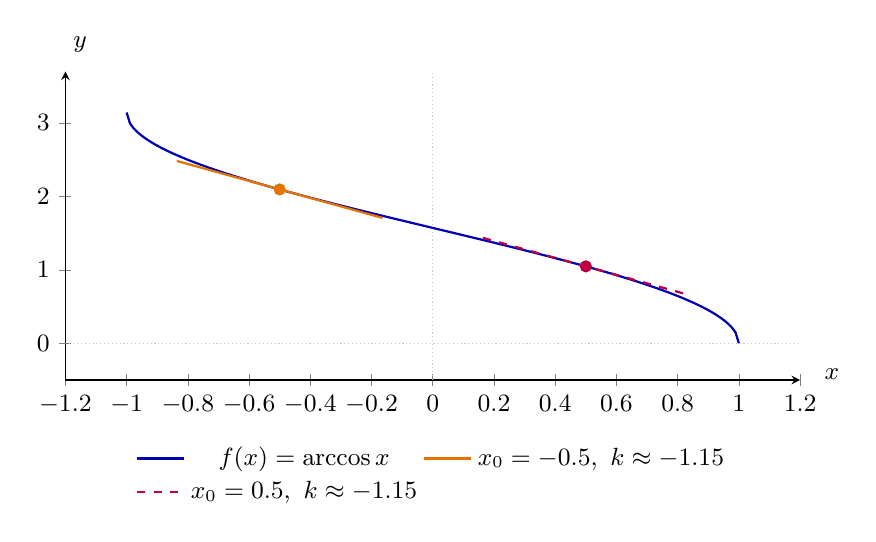
\begin{tikzpicture}[font=\small,>=stealth]
\begin{axis}[width=.90\linewidth,height=5.5cm,xmin=-1.2,xmax=1.2,ymin=-0.5,ymax=3.7,
axis lines=left,xlabel={$x$},ylabel={$y$},font=\small,
xlabel style={at={(axis description cs:1.02,.02)},anchor=west},
ylabel style={rotate=-90,at={(axis description cs:.02,1.03)},anchor=south},
legend style={at={(axis description cs:.5,-.18)},anchor=north,draw=none,fill=none,font=\small,legend columns=2},
unbounded coords=jump,clip=true,]
\addplot[gray!45,thin,densely dotted,forget plot] coordinates {(-1.2,0) (1.2,0)};
\addplot[gray!45,thin,densely dotted,forget plot] coordinates {(0,-0.5) (0,3.7)};
\addplot[blue!70!black,thick] coordinates {(-1,3.1415927) (-0.98888889,2.9923831) (-0.97777778,2.9303818) (-0.96666667,2.8826711) (-0.95555556,2.8423348) (-0.94444444,2.8066965) (-0.93333333,2.7743846) (-0.92222222,2.7445852) (-0.91111111,2.7167682) (-0.9,2.6905658) (-0.88888889,2.6657104) (-0.87777778,2.642) (-0.86666667,2.6192778) (-0.85555556,2.5974193) (-0.84444444,2.5763235) (-0.83333333,2.5559071) (-0.82222222,2.5361008) (-0.81111111,2.5168456) (-0.8,2.4980915) (-0.78888889,2.4797952) (-0.77777778,2.4619188) (-0.76666667,2.4444295) (-0.75555556,2.4272981) (-0.74444444,2.4104987) (-0.73333333,2.3940083) (-0.72222222,2.3778062) (-0.71111111,2.3618736) (-0.7,2.3461938) (-0.68888889,2.3307514) (-0.67777778,2.3155324) (-0.66666667,2.300524) (-0.65555556,2.2857144) (-0.64444444,2.2710928) (-0.63333333,2.2566493) (-0.62222222,2.2423745) (-0.61111111,2.2282599) (-0.6,2.2142974) (-0.58888889,2.2004797) (-0.57777778,2.1867997) (-0.56666667,2.173251) (-0.55555556,2.1598273) (-0.54444444,2.146523) (-0.53333333,2.1333326) (-0.52222222,2.120251) (-0.51111111,2.1072733) (-0.5,2.0943951) (-0.48888889,2.0816119) (-0.47777778,2.0689197) (-0.46666667,2.0563144) (-0.45555556,2.0437925) (-0.44444444,2.0313503) (-0.43333333,2.0189845) (-0.42222222,2.0066917) (-0.41111111,1.9944689) (-0.4,1.9823132) (-0.38888889,1.9702216) (-0.37777778,1.9581914) (-0.36666667,1.9462199) (-0.35555556,1.9343047) (-0.34444444,1.9224433) (-0.33333333,1.9106332) (-0.32222222,1.8988723) (-0.31111111,1.8871583) (-0.3,1.875489) (-0.28888889,1.8638624) (-0.27777778,1.8522764) (-0.26666667,1.8407291) (-0.25555556,1.8292186) (-0.24444444,1.817743) (-0.23333333,1.8063006) (-0.22222222,1.7948894) (-0.21111111,1.7835079) (-0.2,1.7721542) (-0.18888889,1.7608269) (-0.17777778,1.7495241) (-0.16666667,1.7382444) (-0.15555556,1.7269862) (-0.14444444,1.7157478) (-0.13333333,1.7045279) (-0.12222222,1.6933249) (-0.11111111,1.6821373) (-0.1,1.6709637) (-0.088888889,1.6598027) (-0.077777778,1.6486527) (-0.066666667,1.6375125) (-0.055555556,1.6263805) (-0.044444444,1.6152554) (-0.033333333,1.6041358) (-0.022222222,1.5930204) (-0.011111111,1.5819077) (0,1.5707963) (0.011111111,1.559685) (0.022222222,1.5485723) (0.033333333,1.5374568) (0.044444444,1.5263372) (0.055555556,1.5152122) (0.066666667,1.5040802) (0.077777778,1.4929399) (0.088888889,1.48179) (0.1,1.4706289) (0.11111111,1.4594553) (0.12222222,1.4482677) (0.13333333,1.4370647) (0.14444444,1.4258448) (0.15555556,1.4146065) (0.16666667,1.4033482) (0.17777778,1.3920685) (0.18888889,1.3807658) (0.2,1.3694384) (0.21111111,1.3580848) (0.22222222,1.3467032) (0.23333333,1.3352921) (0.24444444,1.3238496) (0.25555556,1.312374) (0.26666667,1.3008635) (0.27777778,1.2893163) (0.28888889,1.2777303) (0.3,1.2661037) (0.31111111,1.2544344) (0.32222222,1.2427204) (0.33333333,1.2309594) (0.34444444,1.2191494) (0.35555556,1.2072879) (0.36666667,1.1953727) (0.37777778,1.1834013) (0.38888889,1.1713711) (0.4,1.1592795) (0.41111111,1.1471237) (0.42222222,1.134901) (0.43333333,1.1226082) (0.44444444,1.1102423) (0.45555556,1.0978001) (0.46666667,1.0852782) (0.47777778,1.072673) (0.48888889,1.0599807) (0.5,1.0471976) (0.51111111,1.0343193) (0.52222222,1.0213417) (0.53333333,1.0082601) (0.54444444,0.99506968) (0.55555556,0.98176536) (0.56666667,0.96834169) (0.57777778,0.95479293) (0.58888889,0.94111295) (0.6,0.92729522) (0.61111111,0.91333277) (0.62222222,0.89921815) (0.63333333,0.88494336) (0.64444444,0.87049981) (0.65555556,0.85587825) (0.66666667,0.84106867) (0.67777778,0.82606025) (0.68888889,0.81084124) (0.7,0.79539883) (0.71111111,0.77971903) (0.72222222,0.7637865) (0.73333333,0.74758435) (0.74444444,0.73109394) (0.75555556,0.71429455) (0.76666667,0.69716313) (0.77777778,0.67967382) (0.78888889,0.66179748) (0.8,0.64350111) (0.81111111,0.62474702) (0.82222222,0.6054919) (0.83333333,0.58568554) (0.84444444,0.56526918) (0.85555556,0.54417334) (0.86666667,0.52231482) (0.87777778,0.49959266) (0.88888889,0.47588225) (0.9,0.45102681) (0.91111111,0.42482443) (0.92222222,0.39700745) (0.93333333,0.36720802) (0.94444444,0.33489616) (0.95555556,0.29925782) (0.96666667,0.25892154) (0.97777778,0.21121088) (0.98888889,0.14920957) (1,0)};
\addlegendentry{$f(x)=\arccos x$}
\addplot[orange!90!black,thick] coordinates {(-0.836,2.4823745) (-0.164,1.7064157)};
\addlegendentry{$x_0=-0.5,\ k\approx-1.15$}
\addplot[only marks,mark=*,orange!90!black,forget plot] coordinates {(-0.5,2.0943951)};
\addplot[purple,thick,dashed] coordinates {(0.164,1.4351769) (0.836,0.65921817)};
\addlegendentry{$x_0=0.5,\ k\approx-1.15$}
\addplot[only marks,mark=*,purple,forget plot] coordinates {(0.5,1.0471976)};

\end{axis}
\end{tikzpicture}
\par\smallskip{\small 拓展；$|x|<1$，导数为负，图像递减。}
\end{center}

\end{minipage}
\end{statementbox}

\begin{statementbox}
\begin{minipage}{\linewidth}
\textbf{结论22：反正切（拓展）}
\[
(\arctan x)'=1/(1+x^2)
\]
% F049: native TikZ/PGFPlots, computed from the stated mathematical model.
\begin{center}
\begin{tikzpicture}[font=\small,>=stealth]
\begin{axis}[width=.90\linewidth,height=5.5cm,xmin=-3.3,xmax=3.3,ymin=-1.8,ymax=1.8,
axis lines=left,xlabel={$x$},ylabel={$y$},font=\small,
xlabel style={at={(axis description cs:1.02,.02)},anchor=west},
ylabel style={rotate=-90,at={(axis description cs:.02,1.03)},anchor=south},
legend style={at={(axis description cs:.5,-.18)},anchor=north,draw=none,fill=none,font=\small,legend columns=2},
unbounded coords=jump,clip=true,]
\addplot[gray!45,thin,densely dotted,forget plot] coordinates {(-3.3,0) (3.3,0)};
\addplot[gray!45,thin,densely dotted,forget plot] coordinates {(0,-1.8) (0,1.8)};
\addplot[blue!70!black,thick] coordinates {(-3,-1.2490458) (-2.9666667,-1.2456788) (-2.9333333,-1.2422432) (-2.9,-1.2387369) (-2.8666667,-1.2351578) (-2.8333333,-1.2315037) (-2.8,-1.2277724) (-2.7666667,-1.2239614) (-2.7333333,-1.2200684) (-2.7,-1.2160907) (-2.6666667,-1.2120257) (-2.6333333,-1.2078706) (-2.6,-1.2036225) (-2.5666667,-1.1992785) (-2.5333333,-1.1948354) (-2.5,-1.1902899) (-2.4666667,-1.1856388) (-2.4333333,-1.1808785) (-2.4,-1.1760052) (-2.3666667,-1.1710152) (-2.3333333,-1.1659045) (-2.3,-1.160669) (-2.2666667,-1.1553042) (-2.2333333,-1.1498058) (-2.2,-1.1441688) (-2.1666667,-1.1383886) (-2.1333333,-1.1324598) (-2.1,-1.1263771) (-2.0666667,-1.120135) (-2.0333333,-1.1137276) (-2,-1.1071487) (-1.9666667,-1.1003921) (-1.9333333,-1.0934509) (-1.9,-1.0863184) (-1.8666667,-1.0789872) (-1.8333333,-1.0714496) (-1.8,-1.0636978) (-1.7666667,-1.0557235) (-1.7333333,-1.047518) (-1.7,-1.0390723) (-1.6666667,-1.0303768) (-1.6333333,-1.0214218) (-1.6,-1.012197) (-1.5666667,-1.0026916) (-1.5333333,-0.99289439) (-1.5,-0.98279372) (-1.4666667,-0.97237743) (-1.4333333,-0.96163286) (-1.4,-0.95054684) (-1.3666667,-0.93910569) (-1.3333333,-0.92729522) (-1.3,-0.9151007) (-1.2666667,-0.90250691) (-1.2333333,-0.8894981) (-1.2,-0.87605805) (-1.1666667,-0.86217005) (-1.1333333,-0.84781697) (-1.1,-0.83298127) (-1.0666667,-0.81764505) (-1.0333333,-0.80179014) (-1,-0.78539816) (-0.96666667,-0.76845063) (-0.93333333,-0.75092906) (-0.9,-0.7328151) (-0.86666667,-0.7140907) (-0.83333333,-0.69473828) (-0.8,-0.67474094) (-0.76666667,-0.65408272) (-0.73333333,-0.63274884) (-0.7,-0.61072596) (-0.66666667,-0.5880026) (-0.63333333,-0.56456939) (-0.6,-0.5404195) (-0.56666667,-0.51554901) (-0.53333333,-0.48995733) (-0.5,-0.46364761) (-0.46666667,-0.43662716) (-0.43333333,-0.40890783) (-0.4,-0.38050638) (-0.36666667,-0.35144479) (-0.33333333,-0.32175055) (-0.3,-0.29145679) (-0.26666667,-0.26060239) (-0.23333333,-0.22923193) (-0.2,-0.19739556) (-0.16666667,-0.16514868) (-0.13333333,-0.13255153) (-0.1,-0.099668652) (-0.066666667,-0.066568164) (-0.033333333,-0.033320996) (0,0) (0.033333333,0.033320996) (0.066666667,0.066568164) (0.1,0.099668652) (0.13333333,0.13255153) (0.16666667,0.16514868) (0.2,0.19739556) (0.23333333,0.22923193) (0.26666667,0.26060239) (0.3,0.29145679) (0.33333333,0.32175055) (0.36666667,0.35144479) (0.4,0.38050638) (0.43333333,0.40890783) (0.46666667,0.43662716) (0.5,0.46364761) (0.53333333,0.48995733) (0.56666667,0.51554901) (0.6,0.5404195) (0.63333333,0.56456939) (0.66666667,0.5880026) (0.7,0.61072596) (0.73333333,0.63274884) (0.76666667,0.65408272) (0.8,0.67474094) (0.83333333,0.69473828) (0.86666667,0.7140907) (0.9,0.7328151) (0.93333333,0.75092906) (0.96666667,0.76845063) (1,0.78539816) (1.0333333,0.80179014) (1.0666667,0.81764505) (1.1,0.83298127) (1.1333333,0.84781697) (1.1666667,0.86217005) (1.2,0.87605805) (1.2333333,0.8894981) (1.2666667,0.90250691) (1.3,0.9151007) (1.3333333,0.92729522) (1.3666667,0.93910569) (1.4,0.95054684) (1.4333333,0.96163286) (1.4666667,0.97237743) (1.5,0.98279372) (1.5333333,0.99289439) (1.5666667,1.0026916) (1.6,1.012197) (1.6333333,1.0214218) (1.6666667,1.0303768) (1.7,1.0390723) (1.7333333,1.047518) (1.7666667,1.0557235) (1.8,1.0636978) (1.8333333,1.0714496) (1.8666667,1.0789872) (1.9,1.0863184) (1.9333333,1.0934509) (1.9666667,1.1003921) (2,1.1071487) (2.0333333,1.1137276) (2.0666667,1.120135) (2.1,1.1263771) (2.1333333,1.1324598) (2.1666667,1.1383886) (2.2,1.1441688) (2.2333333,1.1498058) (2.2666667,1.1553042) (2.3,1.160669) (2.3333333,1.1659045) (2.3666667,1.1710152) (2.4,1.1760052) (2.4333333,1.1808785) (2.4666667,1.1856388) (2.5,1.1902899) (2.5333333,1.1948354) (2.5666667,1.1992785) (2.6,1.2036225) (2.6333333,1.2078706) (2.6666667,1.2120257) (2.7,1.2160907) (2.7333333,1.2200684) (2.7666667,1.2239614) (2.8,1.2277724) (2.8333333,1.2315037) (2.8666667,1.2351578) (2.9,1.2387369) (2.9333333,1.2422432) (2.9666667,1.2456788) (3,1.2490458)};
\addlegendentry{$f(x)=\arctan x$}
\addplot[orange!90!black,thick] coordinates {(-0.924,-0.924) (0.924,0.924)};
\addlegendentry{$x_0=0,\ k=1$}
\addplot[only marks,mark=*,orange!90!black,forget plot] coordinates {(0,0)};
\addplot[purple,thick,dashed] coordinates {(0.076,0.32339816) (1.924,1.2473982)};
\addlegendentry{$x_0=1,\ k=0.5$}
\addplot[only marks,mark=*,purple,forget plot] coordinates {(1,0.78539816)};

\end{axis}
\end{tikzpicture}
\par\smallskip{\small 拓展；$x\in\mathbb R$，越远离原点，切线越平缓。}
\end{center}

\end{minipage}
\end{statementbox}

\begin{statementbox}
\begin{minipage}{\linewidth}
\textbf{结论23：线性组合}
\[
(c_1f_1+c_2f_2)'=c_1f_1'+c_2f_2'
\]
% F049: native TikZ/PGFPlots, computed from the stated mathematical model.
\begin{center}
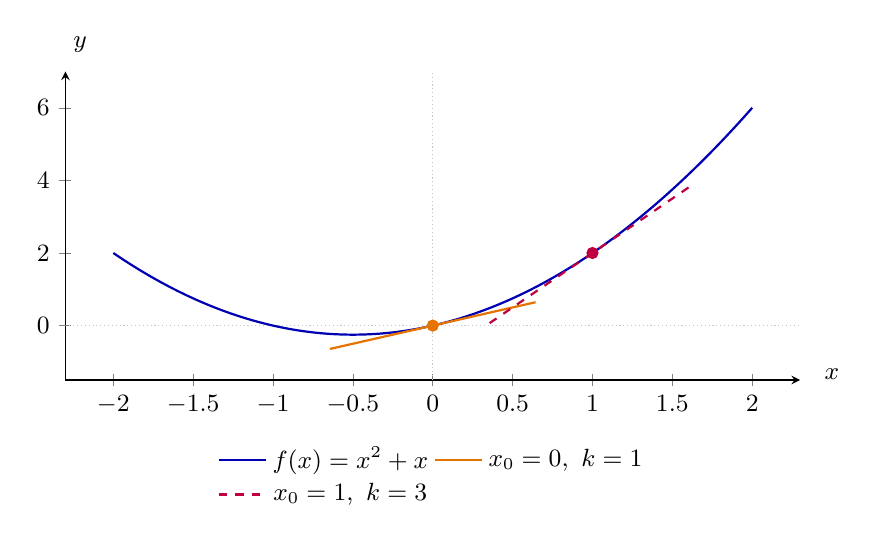
\begin{tikzpicture}[font=\small,>=stealth]
\begin{axis}[width=.90\linewidth,height=5.5cm,xmin=-2.3,xmax=2.3,ymin=-1.5,ymax=7,
axis lines=left,xlabel={$x$},ylabel={$y$},font=\small,
xlabel style={at={(axis description cs:1.02,.02)},anchor=west},
ylabel style={rotate=-90,at={(axis description cs:.02,1.03)},anchor=south},
legend style={at={(axis description cs:.5,-.18)},anchor=north,draw=none,fill=none,font=\small,legend columns=2},
unbounded coords=jump,clip=true,]
\addplot[gray!45,thin,densely dotted,forget plot] coordinates {(-2.3,0) (2.3,0)};
\addplot[gray!45,thin,densely dotted,forget plot] coordinates {(0,-1.5) (0,7)};
\addplot[blue!70!black,thick] coordinates {(-2,2) (-1.9777778,1.9338272) (-1.9555556,1.868642) (-1.9333333,1.8044444) (-1.9111111,1.7412346) (-1.8888889,1.6790123) (-1.8666667,1.6177778) (-1.8444444,1.5575309) (-1.8222222,1.4982716) (-1.8,1.44) (-1.7777778,1.382716) (-1.7555556,1.3264198) (-1.7333333,1.2711111) (-1.7111111,1.2167901) (-1.6888889,1.1634568) (-1.6666667,1.1111111) (-1.6444444,1.0597531) (-1.6222222,1.0093827) (-1.6,0.96) (-1.5777778,0.91160494) (-1.5555556,0.86419753) (-1.5333333,0.81777778) (-1.5111111,0.77234568) (-1.4888889,0.72790123) (-1.4666667,0.68444444) (-1.4444444,0.64197531) (-1.4222222,0.60049383) (-1.4,0.56) (-1.3777778,0.52049383) (-1.3555556,0.48197531) (-1.3333333,0.44444444) (-1.3111111,0.40790123) (-1.2888889,0.37234568) (-1.2666667,0.33777778) (-1.2444444,0.30419753) (-1.2222222,0.27160494) (-1.2,0.24) (-1.1777778,0.20938272) (-1.1555556,0.17975309) (-1.1333333,0.15111111) (-1.1111111,0.12345679) (-1.0888889,0.096790123) (-1.0666667,0.071111111) (-1.0444444,0.046419753) (-1.0222222,0.022716049) (-1,0) (-0.97777778,-0.021728395) (-0.95555556,-0.042469136) (-0.93333333,-0.062222222) (-0.91111111,-0.080987654) (-0.88888889,-0.098765432) (-0.86666667,-0.11555556) (-0.84444444,-0.13135802) (-0.82222222,-0.14617284) (-0.8,-0.16) (-0.77777778,-0.17283951) (-0.75555556,-0.18469136) (-0.73333333,-0.19555556) (-0.71111111,-0.2054321) (-0.68888889,-0.21432099) (-0.66666667,-0.22222222) (-0.64444444,-0.2291358) (-0.62222222,-0.23506173) (-0.6,-0.24) (-0.57777778,-0.24395062) (-0.55555556,-0.24691358) (-0.53333333,-0.24888889) (-0.51111111,-0.24987654) (-0.48888889,-0.24987654) (-0.46666667,-0.24888889) (-0.44444444,-0.24691358) (-0.42222222,-0.24395062) (-0.4,-0.24) (-0.37777778,-0.23506173) (-0.35555556,-0.2291358) (-0.33333333,-0.22222222) (-0.31111111,-0.21432099) (-0.28888889,-0.2054321) (-0.26666667,-0.19555556) (-0.24444444,-0.18469136) (-0.22222222,-0.17283951) (-0.2,-0.16) (-0.17777778,-0.14617284) (-0.15555556,-0.13135802) (-0.13333333,-0.11555556) (-0.11111111,-0.098765432) (-0.088888889,-0.080987654) (-0.066666667,-0.062222222) (-0.044444444,-0.042469136) (-0.022222222,-0.021728395) (0,0) (0.022222222,0.022716049) (0.044444444,0.046419753) (0.066666667,0.071111111) (0.088888889,0.096790123) (0.11111111,0.12345679) (0.13333333,0.15111111) (0.15555556,0.17975309) (0.17777778,0.20938272) (0.2,0.24) (0.22222222,0.27160494) (0.24444444,0.30419753) (0.26666667,0.33777778) (0.28888889,0.37234568) (0.31111111,0.40790123) (0.33333333,0.44444444) (0.35555556,0.48197531) (0.37777778,0.52049383) (0.4,0.56) (0.42222222,0.60049383) (0.44444444,0.64197531) (0.46666667,0.68444444) (0.48888889,0.72790123) (0.51111111,0.77234568) (0.53333333,0.81777778) (0.55555556,0.86419753) (0.57777778,0.91160494) (0.6,0.96) (0.62222222,1.0093827) (0.64444444,1.0597531) (0.66666667,1.1111111) (0.68888889,1.1634568) (0.71111111,1.2167901) (0.73333333,1.2711111) (0.75555556,1.3264198) (0.77777778,1.382716) (0.8,1.44) (0.82222222,1.4982716) (0.84444444,1.5575309) (0.86666667,1.6177778) (0.88888889,1.6790123) (0.91111111,1.7412346) (0.93333333,1.8044444) (0.95555556,1.868642) (0.97777778,1.9338272) (1,2) (1.0222222,2.0671605) (1.0444444,2.1353086) (1.0666667,2.2044444) (1.0888889,2.2745679) (1.1111111,2.345679) (1.1333333,2.4177778) (1.1555556,2.4908642) (1.1777778,2.5649383) (1.2,2.64) (1.2222222,2.7160494) (1.2444444,2.7930864) (1.2666667,2.8711111) (1.2888889,2.9501235) (1.3111111,3.0301235) (1.3333333,3.1111111) (1.3555556,3.1930864) (1.3777778,3.2760494) (1.4,3.36) (1.4222222,3.4449383) (1.4444444,3.5308642) (1.4666667,3.6177778) (1.4888889,3.705679) (1.5111111,3.7945679) (1.5333333,3.8844444) (1.5555556,3.9753086) (1.5777778,4.0671605) (1.6,4.16) (1.6222222,4.2538272) (1.6444444,4.348642) (1.6666667,4.4444444) (1.6888889,4.5412346) (1.7111111,4.6390123) (1.7333333,4.7377778) (1.7555556,4.8375309) (1.7777778,4.9382716) (1.8,5.04) (1.8222222,5.142716) (1.8444444,5.2464198) (1.8666667,5.3511111) (1.8888889,5.4567901) (1.9111111,5.5634568) (1.9333333,5.6711111) (1.9555556,5.7797531) (1.9777778,5.8893827) (2,6)};
\addlegendentry{$f(x)=x^2+x$}
\addplot[orange!90!black,thick] coordinates {(-0.644,-0.644) (0.644,0.644)};
\addlegendentry{$x_0=0,\ k=1$}
\addplot[only marks,mark=*,orange!90!black,forget plot] coordinates {(0,0)};
\addplot[purple,thick,dashed] coordinates {(0.356,0.068) (1.644,3.932)};
\addlegendentry{$x_0=1,\ k=3$}
\addplot[only marks,mark=*,purple,forget plot] coordinates {(1,2)};

\end{axis}
\end{tikzpicture}
\par\smallskip{\small 在各项均可导处成立；图中取 $f_1=x^2,f_2=x,c_1=c_2=1$。}
\end{center}

\end{minipage}
例如 $f=x^3+2e^x-3\ln x+\sin x$（$x>0$），则 $f\prime=3x^2+2e^x-3/x+\cos x$。
七条核心公式的导数定义证明见证明第一部分；其余公式及范围说明见第二部分。
\end{statementbox}

